%
% Modelo de trabalho acadêmico monográfico (Tese de Doutorado, Dissertação de Mestrado
% ou Projeto de Qualificação) em português brasileiro e em conformidade com as normas da ABNT
%
% Documento principal
% Data: 07 de outubro de 2014
%
% *****************************************************************************
% *  Centro Federal de Educação Tecnológica de Minas Gerais - CEFET-MG        *
% *  Laboratório de Sistemas Inteligentes - LSI                               *
% *                                                                           *
% *  Autor: Henrique E. Borges <henrique@lsi.cefetmg.br>                      *
% *  Autor: Denise de Souza <densouza@gmail.com>                              *
% *  Autor: Cristiano Fraga G. Nunes <cfgnunes@gmail.com>                     *
% *  Autor: Lauro César <https://code.google.com/p/abntex2/>                  *
% *                                                                           *
% *****************************************************************************



\documentclass[
      %twoside,					% Impressão em frente (anverso) e verso. Oposto a oneside
      oneside,					% Impressão apenas no anverso. Oposto a twoside
      a4paper,					% Tamanho do papel
%   opções do pacote babel
      english,					% Idioma adicional para hifenização
      brazilian,				% O ultimo idioma indicado será o principal idioma do documento    
]{abntex2-cefetmg} 




% -----------------------------------------------------------------------------
%    Configura as citações bibliográficas conforme a norma ABNT
% -----------------------------------------------------------------------------

\usepackage[brazilian,hyperpageref]{backref}
\usepackage[alf, 
abnt-emphasize=bf, 
bibjustif, 
recuo=0cm,
abnt-doi=expand,                % Expande um endereço iniciado com doi: para http://dx.doi.org/
abnt-url-package=url,           % utiliza o pacote url
abnt-refinfo=yes,               % utiliza o estilo bibliográfico abnt-refinfo
abnt-etal-cite=3, 
abnt-etal-list=3,
abnt-thesis-year=final]{abntex2cite}	% Formata as citações bibliográficas conforme a norma ABNT


% -----------------------------------------------------------------------------
%    Pacotes utilizados 
% -----------------------------------------------------------------------------

%\usepackage[latin1]{inputenc}	% Codificação do documento (conversão automatica dos acentos)
\usepackage[utf8]{inputenc}		% Codificação do documento (conversão automatica dos acentos)
\usepackage[T1]{fontenc}		% Seleção de código de fonte
%\usepackage{times}				% Usa a fonte Times
%\usepackage{lmodern}			% Usa a fonte Latin Modern
%\usepackage{palatino}			% Usa a fonte Palatino
%\usepackage{lmodern}			% Usa a fonte Latin Modern
\usepackage{scalefnt}			% Permite redimensionar tamanho da fonte
\usepackage[scaled]{helvet}		% Usa a fonte Helvetica (default)
	\renewcommand*\familydefault{\sfdefault} 	
%\usepackage{ae,aecompl}		% Fontes de alta qualidade
\usepackage{upgreek}			% Permite inserção de letras gregas
\usepackage{latexsym}			% Permite inserção de símbolos matemáticos
\usepackage{amsfonts, amssymb, amsmath, dsfont}		% fontes e símbolos matemáticos

\usepackage{lscape}				% Permite páginas em modo "paisagem"
\usepackage{indentfirst}		% Indenta o primeiro parágrafo de cada seção.
\usepackage{microtype} 			% Melhora a justificação do documento
\usepackage{hyperref} 			% Usado para criar “hyperlinks” no PDF
%\usepackage[hyphens]{url}    	% Melhora apresentação de URLs
%\usepackage{url}              	% Melhora apresentação de URLs
\usepackage{breakurl}			% Permite quebra de linha em URLs longas
%\usepackage{balance}			% Balanceia o texto no artigo
\usepackage[bottom]{footmisc}	% Mantém as notas de rodapé sempre na mesma posição
\usepackage{verbatim}			% Permite apresentar texto tal como escrito no documento, ainda que sejam comandos Latex
%\usepackage{lettrine} 			% Lettrine é a primeira letra do início de um texto que é aumentada em relação às demais
%\usepackage[pointedenum]{paralist} 		% Usado elaborar listas numeradas ou de “bullets”, aninhadas ou não 

\usepackage{graphicx}			% Inclusão de gráficos e figuras
%\usepackage{subfig}			% Permite posicionar figuras
%\usepackage{picinpar}			% Permite posicionar imagens em parágrafos
%\usepackage{psfrag}			% Inclusão de símbolos latex em figuras eps
\usepackage{tikz}	 			% Pacote para desenhos
\usepackage{color, colortbl}	% Controle das cores
\usepackage{booktabs}			% Réguas horizontais em tabelas
\usepackage{multirow, array}	% Permite tabelas com múltiplas linhas e colunas
\usepackage[algoruled, portuguese]{algorithm2e}		% Permite escrever algoritmos em português
\usepackage{float}				% Necessário para tabelas/figuras em ambiente multi-colunas
								% Devem ser, necessariamente, colocados em pontos específicos junto com [H] (e.g., \begin{table}[H])
\usepackage{subeqnarray}		% Permite subnumeracao de equações

%\usepackage{comandos} 			% Novos comandos
%\usepackage{etoolbox}	 		% Pacote para tratamento de condicionais (if-else-end \ string)
%\usepackage{ifthen}				% Pacote para tratamento de condicionais (if-else-end \ number)

%\usepackage{babel}				% Usado para definir idioma do documento e respectivas hifenizações

\usepackage{bookmark}			% Cria menu de bookmarks
%\usepackage{nomencl} 			% Usado para produzir lista de símbolos
\usepackage{makeidx}			% Usado para produzir índice remissivo (glossário)
	\makeindex 					% Compila o índice
	
%\usepackage{multind}			% Usado para produzir índices múltiplos
%\usepackage{acronym}			% Usado para produzir acrônimos
%\usepackage{bibentry}			% Permite uso de bibtex inline
\usepackage{listings}
%\usepackage{enumerate}
\usepackage{graphicx}
\usepackage{subcaption}
\usepackage{color}
\usepackage{enumitem}
%\setlist[enumerate]{itemsep=0mm}
\definecolor{mygreen}{rgb}{0,0.6,0}
\definecolor{mygray}{rgb}{0.5,0.5,0.5}
\definecolor{mymauve}{rgb}{0.58,0,0.82}

\lstset{ %
  backgroundcolor=\color{white},   % choose the background color; you must add \usepackage{color} or \usepackage{xcolor}; should come as last argument
  basicstyle=\footnotesize,        % the size of the fonts that are used for the code
  breakatwhitespace=false,         % sets if automatic breaks should only happen at whitespace
  breaklines=true,                 % sets automatic line breaking
  captionpos=b,                    % sets the caption-position to bottom
  commentstyle=\color{mygreen},    % comment style
  deletekeywords={...},            % if you want to delete keywords from the given language
  escapeinside={\%*}{*)},          % if you want to add LaTeX within your code
  extendedchars=true,              % lets you use non-ASCII characters; for 8-bits encodings only, does not work with UTF-8
  frame=single,	                   % adds a frame around the code
  keepspaces=true,                 % keeps spaces in text, useful for keeping indentation of code (possibly needs columns=flexible)
  keywordstyle=\color{blue},       % keyword style
  numbers=left,                    % where to put the line-numbers; possible values are (none, left, right)
  numberstyle=\tiny\color{mygray}, % the style that is used for the line-numbers
  rulecolor=\color{black},         % if not set, the frame-color may be changed on line-breaks within not-black text (e.g. comments (green here))
  showspaces=false,                % show spaces everywhere adding particular underscores; it overrides 'showstringspaces'
  showstringspaces=false,          % underline spaces within strings only
  showtabs=false,                  % show tabs within strings adding particular underscores
  stringstyle=\color{mymauve},     % string literal style
  tabsize=2,	                   % sets default tabsize to 2 spaces
  title=\lstname                   % show the filename of files included with \lstinputlisting; also try caption instead of title
}

\renewcommand{\lstlistingname}{Programa}


%   Insere e constroi alguns elementos pré-textuais para gerar capa, folha de rosto e fe folha de aprovação

% -----------------------------------------------------------------------------
%   Arquivo: ./01-elementos-pre-textuais/capa.tex
% -----------------------------------------------------------------------------



% -----------------------------------------------------------------------------
%   ATENÇÃO:
%   Caso algum campo não se aplique ao seu documento - por exemplo, em seu trabalho
%   não houve coorientador - não comente o campo, apenas deixe vazio, assim: \campo{}
% -----------------------------------------------------------------------------



% -----------------------------------------------------------------------------
%   Dados do trabalho acadêmico
% -----------------------------------------------------------------------------

\titulo{Sistema multi-agentes distribuído para simulação de forrageamento de criaturas artificiais com sistema nervoso}
%\title{Title in English}
\subtitulo{}
\autor{Felipe Duarte dos Reis}
\local{Belo Horizonte}
\data{Novembro de 2017}			% normalmente se usa apenas mês e ano



% -----------------------------------------------------------------------------
%   Natureza do trabalho acadêmico
%   Use apenas uma das opções: Tese (p/ Doutorado), Dissertação (p/ Mestrado) ou
%   Projeto de Qualificação (p/ Mestrado ou Doutorado), Trabalho de Conclusão de
%   Curso (Graduação)
% -----------------------------------------------------------------------------

\projeto{Trabalho de Conclusão de Curso}



% -----------------------------------------------------------------------------
%   Título acadêmico
%   Use apenas uma das opções:
%	Se a natureza for Tese, coloque Doutor
%	Se a natureza for Dissertação, coloque Mestre
%	Se a natureza for Projeto de Qualificação, coloque Mestre ou Doutor conforme o caso
%   Se a natureza for Trabalho de Conclusão de Curso, coloque Bacharel
% -----------------------------------------------------------------------------

\tituloAcademico{Bacharel}



% -----------------------------------------------------------------------------
%   Área de concentração e linha de pesquisa
%	OBS: indique o nome da área de concentração e da linha de pesquisa do Programa de Pós-graduação
%   nas quais este trabalho se insere
%   Se a natureza for Trabalho de Conclusão de Curso, deixe ambos os campos vazios
% -----------------------------------------------------------------------------


\areaconcentracao{}
\linhapesquisa{}



% -----------------------------------------------------------------------------
%   Dados da instituicao
%   OBS: a logomarca da instituiçã deve ser colocada na mesma pasta que foi colocada o documento
%   principal com o nome de "logoInstituicao". O formato pode ser: pdf, jpf, eps
%   Se a natureza for Trabalho de Conclusão de Curso, coloque em "programa' o nome do curso de graduação
% -----------------------------------------------------------------------------

\instituicao{Centro Federal de Educação Tecnológica de Minas Gerais}
%\programa{Programa de Pós-graduação em Modelagem Matemática e Computacional}
\programa{Curso de Engenharia de Computação}
\logoinstituicao{0.2}{logoInstituicao}                  % \logoinstituicao{<escala>}{<nome do arquivo>}



% -----------------------------------------------------------------------------
%   Dados do(s) orientador(es)
% -----------------------------------------------------------------------------

\orientador{Prof. Dr. Henrique Elias Borges}
%\orientador[Orientadora:]{Nome da orientadora}
\instOrientador{Centro Federal de Educação Tecnológica de Minas Gerais}

\coorientador{}
%\coorientador[Coorientadora:]{Nome da coorientadora}
\instCoorientador{}



% -----------------------------------------------------------------------------
%   Arquivo: ./01-elementos-pre-textuais/folhaRosto.tex
% -----------------------------------------------------------------------------



% -----------------------------------------------------------------------------
%   Trabalho de Conclusão de Curso
% -----------------------------------------------------------------------------

%\preambulo{{\imprimirprojeto} apresentado ao Curso de Engenharia de Computação do Centro Federal de Educação Tecnológica de Minas Gerais, como requisito parcial para a obtenção do título de {\imprimirtituloAcademico} em Engenharia de Computação.}



% -----------------------------------------------------------------------------
%   Projeto de qualificação de Mestrado ou Doutorado
% -----------------------------------------------------------------------------

\preambulo{{\imprimirprojeto} apresentado ao Curso de Engenharia da Computação do Centro Federal de Educação Tecnológica de Minas Gerais, como requisito parcial para a obtenção do título de {\imprimirtituloAcademico} em Engenharia da Computação.}



% -----------------------------------------------------------------------------
%   Dissertação de Mestrado
% -----------------------------------------------------------------------------

%\preambulo{{\imprimirprojeto} apresentada ao Programa de \mbox{Pós-graduação} em Modelagem Matemática e Computacional do Centro Federal de Educação Tecnológica de Minas Gerais, como requisito parcial para a obtenção do título de {\imprimirtituloAcademico} em Modelagem Matemática e Computacional.}



% -----------------------------------------------------------------------------
%   Tese de Doutorado
% -----------------------------------------------------------------------------

%\preambulo{{\imprimirprojeto} apresentada ao Programa de \mbox{Pós-graduação} em Modelagem Matemática e Computacional do Centro Federal de Educação Tecnológica de Minas Gerais, como requisito parcial para a obtenção do título de {\imprimirtituloAcademico} em Modelagem Matemática e Computacional.}




% -----------------------------------------------------------------------------
%   Edite este arquivo comentando as linhas que não se aplicam ao tipo de documento acadêmico pretendido.
% -----------------------------------------------------------------------------
% -----------------------------------------------------------------------------
%   Arquivo: ./01-elementos-pre-textuais/folhaAprovacao.tex
% -----------------------------------------------------------------------------



\textopadraofolhadeaprovacao{Esta folha deverá ser substituída pela cópia digitalizada da folha de aprovação fornecida pelo Programa de Pós-graduação.}



% -----------------------------------------------------------------------------
%  Este documento foi mantido apenas para preservar a paginação do trabalho acadêmico
%  final, após a inserção da folha de arpovação fornecida pelo programa.
% -----------------------------------------------------------------------------





% -----------------------------------------------------------------------------
%   Configurações de aparência do PDF final
% -----------------------------------------------------------------------------

\definecolor{blue}{RGB}{41,5,195}	% Altera o aspecto da cor azul

\makeatletter
\hypersetup{
	portuguese,
    colorlinks=true,       	% true: “links” coloridos; false: “links” em caixas de texto
	linkcolor=blue,			% Define cor dos “links” internos”
	citecolor=blue,			% Define cor dos “links” para as referências bibliográficas
	filecolor=blue,			% Define cor dos “links” para arquivos
	urlcolor=blue, 			% Define a cor dos “hiperlinks”
	breaklinks=true,
	pdftitle={\@title},
	pdfauthor={\@author},
%	pdfsubject={\imprimirpreambulo},
	pdfkeywords={abnt, latex, abntex, abntex2}
}
\makeatother



% -----------------------------------------------------------------------------
%   Hifenização de palavras não constantes do dicionário
% -----------------------------------------------------------------------------

\hyphenation{
		qua-dros-cha-ve
		Bras-nett
		Kat-sa-gge-los
}



% -----------------------------------------------------------------------------
%   Inclui todos os arquivos do trabalho acadêmico
% -----------------------------------------------------------------------------

\begin{document}

\frenchspacing				%   Retira o espaço extra desnecessário nas frases

%   Gera e imprime alguns elementos pré-textuais: capa, folha de rosto e folha de aprovação

\pretextual
\imprimircapa 											% Comando para imprimir Capa
\imprimirfolhaderosto{} 								% Comando para imprimir Folha de rosto
\imprimirfolhadeaprovacao{} 							% Comando para imprimir Folha de aprovação

%   Insere os demais elementos pré-textuais

% -----------------------------------------------------------------------------
%   Arquivo: ./01-elementos-pre-textuais/dedicatoria.tex
% -----------------------------------------------------------------------------



\begin{dedicatoria}
Dedico este trabalho ao meu pai Renato, e a minha mãe Janaina, que me permitiram sonhar ainda quando tudo era adverso. Vocês são a razão  de eu ter chegado onde cheguei.

\end{dedicatoria}

		% Dedicatória
% -----------------------------------------------------------------------------
%   Arquivo: ./01-elementos-pre-textuais/agradecimentos.tex
% -----------------------------------------------------------------------------



\begin{agradecimentos}

Agradeço ao Eterno.

Agradeço ao prof. Dr. Henrique Elias Borges, com quem tenho a sorte de trabalhar a oito anos, e quem me ensinou muito mais do que fazer pesquisa. Obrigado pela paciência durante esses anos de orientação, pelos valiosos ensinamentos e pela persistência em trazer este trabalho até aqui.

Agradeço ao CEFET-MG, a todos os professores do Departamento de Computação, em especial ao prof. Dr. Sandro Renato Dias que se tornou um grande amigo.

Faltam palavras para agradecer meus pais, Renato Bertodo dos Reis e Janaina Ferreira Duarte dos Reis.

Agradeço à Júlia, que esteve ao meu lado nos momentos e decisões mais difíceis ao longo deste último ano de graduação, cuja presença sempre me tranquilizou e nunca faltaram palavras de apoio.

Agradeço aos colegas do Laboratório de Sistemas Inteligentes que acompanharam de perto o desenvolvimento deste trabalho, o Lucas Marioza, o Vitor Peixoto, a Ravilla Noely e o Matheus Galantine. Em especial a duas alunas da pós-graduação: Jahina Assis, que conheci no início do curso e se tornou para mim como uma irmã, e a Carolina Marcelino com quem tive mais contato do meio do curso em diante, e que se tornou uma inspiração de dedicação e sucesso para mim.

Agradeço a outros amigos e colegas que conheci ao longo  do curso e que, de algum modo influenciaram positivamente essa jornada: Bruno Figueiró, Gabriel Poesia, Juan Lopes, Rafael Pacheco, Guilherme Renna, Higor Coimbra, Matheus Almeida, Miguel Felipe, Thales Bacelar, Bárbara Poliana, Rodrigo Novaes, Gustavo Borba, Amanda Barbosa, e a tantos outros que a memória me falha agora mas que não por isso não sejam especiais. 

\end{agradecimentos}
	% Agradecimentos
% -----------------------------------------------------------------------------
%   Arquivo: ./01-elementos-pre-textuais/epigrafe.tex
% -----------------------------------------------------------------------------



\begin{epigrafe}

\textit{``A poesia está guardada nas palavras — é tudo que eu sei.\\
Meu fado é de não saber quase tudo.\\
Sobre o nada eu tenho profundidades.\\
Não tenho conexões com a realidade.\\
Poderoso para mim não é aquele que descobre ouro.\\
Para mim poderoso é aquele que descobre as\\
insignificâncias (do mundo e as nossas).\\
Por essa pequena sentença me elogiaram de imbecil.\\
Fiquei emocionado e chorei.\\
Sou fraco para elogios.''}

(Manoel de Barros)
\end{epigrafe}



% -----------------------------------------------------------------------------
%   Edite o texto acima para inserir uma epígrafe de sua preferência
% -----------------------------------------------------------------------------
			% Epígrafe
% -----------------------------------------------------------------------------
%   Arquivo: ./01-elementos-pre-textuais/resumoPt.tex
% -----------------------------------------------------------------------------



\begin{resumo}

Sistemas multi-agente (MAS) são frequentemente empregados na modelagem e simulação de sistemas ecológicos e biológicos. Uma das aplicações é na simulação de vida artificial, onde uma criatura com sistema nervoso deve explorar um mundo desconhecido e aprender como sobreviver a partir das suas interações com o mundo. Trata-se, pois, de simular computacionalmente um sistema dinâmico, o que exige assincronia dos eventos. Esta exigência revela-se incompatível com o modelo clássico de concorrência que utiliza memória compartilhada, no qual o controle de concorrência é síncrono. Para resolver essa incompatibilidade neste trabalho, utilizamos o modelo de concorrência assíncrona baseado em atores para implementar uma simulação de forrageamento de criaturas artificiais com sistema nervoso assíncrono. Na implementação, foi utilizado o \textit{toolkit} Akka, desenvolvido em Java para implementar o mundo e a criatura artificial. Cada circuito de estimulação do sistema nervoso foi implementado e testado separadamente. Um conjunto de experimentos foram realizados visando validar e verificar o correto funcionamento do modelo proposto. Os resultados se mostraram qualitativamente comparáveis e quantitativamente congruentes com a versão anterior da simulação no caso de uma única criatura. O que nos permite considerar validado e verificado o modelo de simulador baseado no modelo de atores. Outros experimentos foram realizados visando explorar preliminarmente aspectos de escalabilidade horizontal e vertical do simulador. 

\begin{comment}
 contexto: simulação de sistemas ecológicos utilizando MAS
 motivação: simular sistemas complexos e de larga escala com plausabilidade biológica
 justificativa: assincronia intrínseca deste tipo de modelo é incompatível com os modelos de programação utilizando memória compartilhada
 objetivo: implementar um simulador escalável utilizando o modelo de atores, bem como um sistema nervoso assíncrono
 metodologia: usar o toolkit akka implementado na linguagem Java para construir o mundo e a criatura artificial, testar os circuitos de estimulação da dinâmica interna, verificar e validar o modela via simulação de forrageamento
 resultado: Escalabilidade. Espera-se fazer as simulações em larga escala e com os resultados compatíveis com a literatura
\end{comment}


\textbf{Palavras-chave}: Sistemas Multi-Agentes. Arquiteturas cognitivas. Modelo de atores.
 

\end{resumo}



% -----------------------------------------------------------------------------
%   Escolha de 3 a 6 palavras ou termos que descrevam bem o seu trabalho. As palavras-chaves são utilizadas para indexação.
%   A letra inicial de cada palavra deve estar em maiúsculas. As palavras-chave são separadas por ponto.
% -----------------------------------------------------------------------------
			% Resumo na língua vernacular
% -----------------------------------------------------------------------------
%   Arquivo: ./01-elementos-pre-textuais/resumoEn.tex
% -----------------------------------------------------------------------------



\begin{resumo}[Abstract]
%Sistemas multi-agente (MAS) são frequentemente empregados na modelagem e simulação de sistemas ecológicos e biológicos. 
Multi-Agent Sistems (MAS) are frequently  used in biological and ecological modeling. 
%Uma das aplicações é na simulação de vida artificial, onde uma criatura com sistema nervoso deve explorar um mundo desconhecido e aprender como sobreviver a partir das suas interações com o mundo. 
Artificial life simulation is one of its aplications, where a criature owed with a nervous system must explorate an unkown world and learn to survive based on interactions with the world.
%Trata-se pois de simular computacionalmente um sistema dinâmico, o que exige assincronia dos eventos. 
It is equivalent to simulate a dynamic system computationally, demanding event asynchrony. 
%Esta exigência revela-se incompatível com o modelo clássico de concorrência que utiliza memória compartilhada, no qual o controle de concorrência é síncrono. 
Such requirement is incompatible with classical concurrence model, based on shared memory and synchronous concurrence control.
%Para resolver essa incompatibilidade neste trabalho utilizamos o modelo de concorrência assíncrona baseado em atores para implementar uma simulação de forrageamento de criaturas artificiais com sistema nervoso assíncrono. 
In order to solve such incompatibility, we take advantage of the asynchronous concurrency model based on actors to implement a foraging simulation with artificial creatures.
%Na implementação foi utilizado o o \textit{toolkit} Akka desenvolvido em Java para implementar o mundo e a criatura artificial. 
The actor model implementation choosen was the Akka toolkit, developed in Java, to build both creature and the artificial world.
%Cada circuito de estimulação do sistema nervoso foi implementado e testado separadamente. 
Each nervous system circuit was implemented and tested separatedly.
%Um conjunto de experimentos foram realizados visando validar e verificar o correto funcionamento do modelo proposto. 
An experiment set was executed aiming to validate and verficiate the functioning of the proposed model.
%Os resultados se mostraram qualitativamente comparáveis e quantitativamente congruentes com a versão anterior da simulação no caso de uma única criatura. 
In the case of one creature the results showed qualitatively comparable and quantitatively congruent with the previous version.
%O que nos permite considerar validado e verificado o modelo de simulador baseado modelo de atores. Outros experimentos foram realizados visando explorar preliminarmente aspectos de escalabilidade horizontal e vertical do simulador. 
That permit us considerate the simulation based on actors validated and verified. Another experiment set were realized to investigate the system scalability.

\textbf{Palavras-chave}: Multi-Agent Systems. Cognitive architectures. Actors model.
 


\end{resumo}



% -----------------------------------------------------------------------------
%   O restante da formatação deve manter-se igual ao do reusmo em português, i.e, um único parágrafo.
% -----------------------------------------------------------------------------
			% Resumo em língua inglesa
% -----------------------------------------------------------------------------
%   Arquivo: ./01-elementos-pre-textuais/listaFiguras.tex
% -----------------------------------------------------------------------------



\pdfbookmark[0]{\listfigurename}{lof}
\listoffigures*
\cleardoublepage



% -----------------------------------------------------------------------------
%   Este arquivo não necessita de ser editado. A lista é gerada automaticamente.
% -----------------------------------------------------------------------------		% Lista de figuras
%% -----------------------------------------------------------------------------
%   Arquivo: ./01-elementos-pre-textuais/listaTabelas.tex
% -----------------------------------------------------------------------------



\pdfbookmark[0]{\listtablename}{lot}
\listoftables*
\cleardoublepage



% -----------------------------------------------------------------------------
%   Este arquivo não necessita de ser editado. A lista é gerada automaticamente.
% -----------------------------------------------------------------------------		% Lista de tabelas
%% -----------------------------------------------------------------------------
%   Arquivo: ./01-elementos-pre-textuais/listaQuadros.tex
% -----------------------------------------------------------------------------



\pdfbookmark[0]{\listofquadrosname}{loq}
\listofquadros*
\cleardoublepage



% -----------------------------------------------------------------------------
%   Este arquivo não necessita de ser editado. A lista é gerada automaticamente.
% -----------------------------------------------------------------------------		% Lista de quadros
%% -----------------------------------------------------------------------------
%   Arquivo: ./01-elementos-pre-textuais/listaAlgoritmos.tex
% -----------------------------------------------------------------------------



\newcommand{\algoritmoname}{Algoritmo}
\renewcommand{\listalgorithmcfname}{Lista de Algoritmos}

\floatname{algocf}{\algoritmoname}
\newlistof{listofalgoritmos}{loa}{\listalgoritmoname}
\newlistentry{algocf}{loa}{0}

\counterwithout{algocf}{chapter}
\renewcommand{\cftalgocfname}{\algoritmoname\space}
\renewcommand*{\cftalgocfaftersnum}{\hfill--\hfill}

\pdfbookmark[0]{\listalgorithmcfname}{loa}
\listofalgorithms
\cleardoublepage



% -----------------------------------------------------------------------------
%   Este arquivo não necessita de ser editado. A lista é gerada automaticamente.
% -----------------------------------------------------------------------------	% Lista de algoritmos
%% -----------------------------------------------------------------------------
%   Arquivo: ./01-elementos-pre-textuais/listaSiglas.tex
% -----------------------------------------------------------------------------



\begin{siglas}
	\item[ABNT] Associação Brasileira de Normas Técnicas
	\item[DECOM] Departamento de Computação
	
	
\end{siglas}



% -----------------------------------------------------------------------------
%   Edite a lista acima para definir "todos" os acrônimos e siglas utilizados neste trabalho
% -----------------------------------------------------------------------------
		% Lista de abreviaturas e siglas
%% -----------------------------------------------------------------------------
%   Arquivo: ./01-elementos-pre-textuais/listaSimbolos.tex
% -----------------------------------------------------------------------------



\begin{simbolos}
	\item[$ \Gamma $] Letra grega Gama
	\item[$ \lambda $] Comprimento de onda
	\item[$ \in $] Pertence


\end{simbolos}



% -----------------------------------------------------------------------------
%   Edite a lista acima para definir "todos" os símbolos utilizados neste trabalho
% -----------------------------------------------------------------------------
		% Lista de símbolos
% -----------------------------------------------------------------------------
%   Arquivo: ./01-elementos-pre-textuais/sumario.tex
% -----------------------------------------------------------------------------



\pdfbookmark[0]{\contentsname}{toc}
\tableofcontents*
\cleardoublepage



% -----------------------------------------------------------------------------
%   Este arquivo não necessita de ser editado. O sumário é gerado automaticamente.
% -----------------------------------------------------------------------------			% Sumário

%   Insere os elementos textuais
\textual
% -----------------------------------------------------------------------------
%   Arquivo: ./02-elementos-textuais/introducao.tex
% -----------------------------------------------------------------------------

\begin{comment}
 contexto: simulação de sistemas ecológicos utilizando MAS
 motivação: simular sistemas complexos e de larga escala com plausabilidade biológica
 justificativa: assincronia intrínseca deste tipo de modelo é incompatível com os modelos de programação utilizando memória compartilhada
 objetivo: implementar um simulador escalável utilizando o modelo de atores, bem como um sistema nervoso assíncrono
 metodologia: usar o toolkit akka implementado na linguagem Java para construir o mundo e a criatura artificial, testar os circuitos de estimulação da dinâmica interna, verificar e validar o modela via simulação de forrageamento
 resultado: Escalabilidade. Espera-se fazer as simulações em larga escala e com os resultados compatíveis com a literatura
\end{comment}

\chapter{Introdução}
\label{chap:introducao}

% Contexto: Sistemas inteligentes, sistemas multi-agentes
Dentre as abordagens propostas na computação para a construção de sistemas inteligentes,
tiveram maior destaque os sistemas especialistas, a lógica fuzzy, as redes neurais artificiais,
sistemas bio-inspirados, e os sistemas multi-agentes (MAS), sendo essas não excludentes. MAS são aplicados na modelagem e simulação de sistemas complexos, \textit{e.g.} sistemas ecológicos, sociais e econômicos, a fim de estudar a emergência de fenômenos na dinâmica do sistema \cite{Niazi2011}. Essa abordagem tem sido aplicada também nos mais diversos setores da indústria e economia com sucesso \cite{Muller2014}.

% Motivação: simular sistemas com plausabilidade biológica em larga escala
Segundo \citeonline{Niazi2011} MAS são frequentemente empregados em modelagem de sistemas ecológicos e biológicos, em especial nas aplicações de vida artificial e cognição. Estudar a emergência de fenômenos como adaptação, aprendizagem, linguagem e consciência é um desafio nessa área de pesquisa \cite{Bedau2000}. \citeonline{Duch2008}  classifica várias arquiteturas cognitivas  baseando-se na abordagem usada na construção de cada uma. Essas classes são: simbólicas, emergentes e híbridas. Arquiteturas simbólicas são baseadas em um processador de símbolos de alto nível, e partem de uma perspectiva \textit{top-down}. Arquiteturas emergentes partem de um fundamento conexionista, baseado em redes neurais e abordam a cognição da perspectiva \textit{bottom-up}. A categoria de arquiteturas híbridas combina ambas as abordagens para produzir um modelo que exiba um comportamento plausível com o fenômeno biológico da cognição, em especial, o que se observa nos seres humanos. Nesta última categoria se enquadram algumas arquiteturas cognitivas multi-agentes populares, como por exemplo, LIDA e CLARION \cite{Franklin2006, Sun2001}. Um outro trabalho baseado na teoria incorporada da cognição é a arquitetura Artífice, apresentada por \citeonline{Campos2015}. Essas arquiteturas em geral são complexas, compostas de vários componentes que interagem entre si, podendo eles serem concorrentes e não-determinísticos, que é o caso da última citada.  

Um modelo fiel de um processo cognitivo é naturalmente complexo e a implementação de uma arquitetura baseada em tal modelo certamente terá um alto custo computacional. \citeonline{Prasad1996} mostraram que ao aumentar a complexidade de um sistema multi-agente acarreta em impactos na sua performance, escalabilidade e estabilidade. O autor também argumenta que a escalabilidade não é um atributo do modelo, e sim, da implementação, e está relacionada principalmente com as tecnologias adotadas. Portanto, para estudar sistemas complexos, principalmente os que modelam fenômenos biológicos, executando simulações em larga escala, é necessário escolher um ferramental tecnológico adequado.

%Justificativa: assincronia intrínseca deste tipo de modelo é incompatível com os modelos de programação utilizando memória compartilhada
Quando a área de estudo envolve sistemas dinâmicos, ecológicos ou qualquer outro processo de origem biológica, como é o caso de processos cognitivos de criaturas artificiais - contexto no qual este trabalho se insere, há dois aspectos que parecem relevantes e devem ser considerados: tais processos são inerentemente não-determinísticos \cite{Symmons2016} e assíncronos \cite{Fisher2008, Strombom2017, Wang2016}. Consequente, um modelo matemático e/ou computacional que vise manter algum grau de plausibilidade biológica para com o fenômeno modelado, deverá c    onsequentemente manter pelo menos uma destas duas características, quais sejam o não-determinismo e a assincronia. Todavia, no que concerne ao aspecto computacional, a larga maioria dos modelos apresentados na literatura recorre ao uso de \textit{threads} e controle de concorrência síncronos. 

O mecanismo de concorrência por \textit{threads} surgiu na década de 70 com o objetivo de produzir sistemas mais confiáveis \cite{Hansen2013}. Uma \textit{thread} é um trecho de código de um programa que pode executar simultaneamente à outros. Quando duas \textit{threads} tentam acessar a mesma posição de memória ao mesmo tempo isso causa uma condição de corrida, produzindo um estado inválido da memória. Para controlar os acessos concorrentes usa-se um mecanismo chamado semáforo binário ou \textit{mutex}, que bloqueia o acesso de uma \textit{thread} enquanto outra está fazendo o acesso. Esse tipo de solução bloqueante não é escalável uma vez que a medida que o número de \textit{threads} cresce, a concorrência pelos recursos compartilhados aumenta, fazendo que o sistema execute praticamente de forma sequencial, o que diminui o desempenho computacional.  

Atualmente outros modelos de concorrência tem surgido, principalmente com a necessidade de se produzir sistemas mais escaláveis. Como por exemplo o modelo de atores \cite{Tasharofi2013, Hewitt2010,  Haller2012}, proposto inicialmente por \citeonline{Hewitt1973} como um formalismo para construção de softwares inteligentes. Um ator é uma primitiva universal da computação digital, não compartilha estado com outros atores e pode se comunicar com estes via troca de mensagens assíncrona. Ao receber uma mensagem um ator pode: alterar seu estado interno, criar um número finito de atores, ou enviar um número finito de mensagens a outro ator. A assincronia intrínseca do modelo de atores permite produzir sistemas mais escaláveis, aproveitando ao máximo vários núcleos de um mesmo computador, bem como vários computadores em um \textit{cluster}. Essa característica do modelo é bem compatível com os sistemas multi-agentes que modelam processos cognitivos, onde os eventos também podem ocorrer de maneira não simultânea.

Apesar de tanto o modelo de atores quando o de \textit{threads} terem surgido praticamente na mesma época, o primeiro começou a ganhar popularidade recentemente com a popularização das aplicações \textit{web} e do \textit{cloud computting}. Uma das implementações mais robustas deste modelo atualmente é o Akka, inicialmente feito em linguagem Scala e, posteriormente na linguagem Java. 

% Objetivo: implementar um simulador escalável utilizando o modelo de atores, bem como um sistema nervoso assíncrono
Tendo em vista a existência de trabalhos na área de sistemas multi-agentes que necessitam de escalabilidade, construídos sobre modelos de concorrência que dificultam o crescimento desses sistemas, e não obstante, existem modelos alternativos de concorrência que favorecem a escalabilidade, cujas características se adaptam bem à simulação de sistemas cognitivos; o que se propõe neste trabalho é utilizar o modelo de atores para construir um simulador de vida artificial, distribuído e assíncrono,  dotado de um sistema nervoso artificial, que seja escalável.  Este simulador será baseado na arquitetura Artífice, citada anteriormente. Posto este objetivo geral, os objetivos específicos do trabalho são:

\begin{enumerate}
    \item Compreender o modelo de atores aplicado a construção de sistemas multi-agentes
    \item Estudar e compreender a arquitetura Artífice 
    \item Apresentar uma nova versão da arquitetura, baseando-se no modelo de atores
    \item Apresentar um modelo de simulação em ambiente distribuído
    \item Implementar o modelo proposto utilizando o \textit{toolkit} Akka
    \item Executar simulações da arquitetura proposta, extraindo dados da execução, para compará-lo com a literatura do projeto Artífice
\end{enumerate}

Feita esta introdução, o trabalho está organizado da seguinte maneira: o \autoref{chap:fundamentacaoTeorica} introduz o modelo de concorrência por estado compartilhado utilizando \textit{threads} e como surgem os principais problemas de sincronização, apresenta o modelo de atores, uma de suas implementações, o \textit{toolkit}  Akka e como ele resolve esses problemas. O \autoref{chap:trabRelac} apresenta uma breve descrição de algumas arquiteturas cognitivas, em destaque a arquitetura Artífice, e como ela se diferencia dos trabalhos na literatura. O \autoref{chap:metodologia} apresenta o a metodologia, bem como o desenvolvimento do trabalho, e as principais escolhas de projeto. Um conjunto de experimentos preliminares e seus resultados é apresentado no \autoref{chap:resultados}  e por fim o  \autoref{chap:conclusao} faz as considerações finais.

			% Introdução
% -----------------------------------------------------------------------------
%   Arquivo: ./02-elementos-textuais/fundamentacaoTeorica.tex
% -----------------------------------------------------------------------------

\chapter{Fundamentação Teórica}
\label{chap:fundamentacaoTeorica}

Neste capítulo serão apresentados conceitos pertinentes para a compreensão do presente trabalho. A \autoref{sec:concorrencia} apresenta os fundamentos de controle de concorrência usando o modelo de \textit{threads}. A \autoref{sec:atores} apresenta o modelo de atores e uma de suas implementações, provendo exemplos que explicam como são eliminados os problemas existentes no clássico de concorrência.

\section{Concorrência usando threads}
\label{sec:concorrencia}

Programação concorrente surge na década de 70 com a necessidade de sistemas operacionais executarem vários processos ao mesmo tempo, e seu desenvolvimento ao longo dos anos teve o objetivo de produzir sistemas mais confiáveis \cite{Hansen2013}. Com ele muitos problemas de pesquisa surgiram, foram abordados e solucionados. Atualmente a maioria das linguagens de programação tem mecanismos consolidados que partiram desse desenvolvimento.

Assim como em um sistema operacional em que muitos processos podem executar concorrentemente, dentro de um mesmo processo várias linhas de execução, doravante \textit{threads}, podem executar ao mesmo tempo. O uso de programação concorrente é fundamental atualmente para fazer uso das arquiteturas \textit{multi-core} modernas. A diferença fundamental entre \textit{threads} é que as primeiras compartilham o mesmo espaço de endereçamento, \textit{i.e.} elas tem acesso às mesmas variáveis e podem executar operações de leitura e escrita nelas simultaneamente. O acesso concorrente a posições na memória compartilhadas sem o devido  controle pode causar problemas a execução de programas \textit{multi-thread}, uma vez que o escalonamento das \textit{threads} é não-determinístico. Os principais problemas que tem de ser controlados são \textit{deadlocks}, \textit{starvation}, e condições de corrida.

Uma \textbf{condição de corrida} acontece quando duas threads entram em uma \textbf{seção crítica} e executam ao mesmo tempo uma operação em memória produzindo um estado inválido. Uma \textbf{seção crítica} é um trecho de código em que a execução de mais de uma \textit{thread} não deve ser permitida \cite[p. 206]{Silberschatz2012}. O \autoref{lst:corrida} mostra um exemplo de código em C que pode exibir um problema de condição de corrida. 

\begin{lstlisting}[language=c,label={lst:corrida},caption={Exemplo de programa \textit{multithread} em C onde ocorre uma condição de corrida}]
#include <pthread.h>
#include <stdio.h>

int cont;

void* inc(void* n) {
    cont = cont + 1;
    return NULL;
}

int main() {
    pthread_t threads[3];
    cont = 0;
    for (int i = 0; i < 3; ++i)
        pthread_create(&threads[i], NULL, &inc, NULL);
    for (int  i = 0; i < 3; ++i)
        pthread_join(threads[i], NULL);
        
    printf("%d\n", cont);
    return 0;
}
\end{lstlisting}

O programa cria três \textit{threads} na linha quinze que executam a função que está definida na linha 6. Essa função simplesmente incrementa o contador global \textbf{cont}. O programa espera todas as \textit{threads} terminarem na linha 17 e exibe o resultado na linha 19. A depender da ordem que os comandos são executados, o resultado final do contador pode não ser igual ao número de \textit{threads} que executaram. A lista abaixo exibe uma ordem das \textit{threads} executadas para \autoref{lst:corrida} que produz o valor final 2 enquanto o esperado seria 3:

\begin{enumerate}
 \item A \textit{thread} 1 lê o valor 0 da variável cont da memória principal
 \item A \textit{thread} 2 lê o valor 0 da variável cont da memória principal
 \item Ambas as \textit{threads} 1 e 2 executam o incremento produzindo o valor 1
 \item A \textit{thread} 1 escreve 1 na variável cont
 \item A \textit{thread} 2 escreve 1 na variável cont
 \item A \textit{thread} 3 executa produzindo o valor 2 na variável cont
\end{enumerate}

Esse problema de ordenação dos comandos pode ser resolvido com uma primitiva de sincronização chamada semáforo binário, ou \textit{mutex}. Essa estrutura controla o acesso à seção crítica, permitindo apenas uma \textit{thread} acessá-la por vez. Se uma segunda \textit{thread} tenta fazer o acesso enquanto primeira está executando a seção crítica, aquela é posta em estado de espera até que o \textit{mutex} seja liberado. 

Quando uma \textit{thread} entra na seção crítica ela deve garantidamente deixar a seção crítica em algum momento, caso contrário as outras \textit{threads} que tentarem acessar a região podem ficar em \textit{\textbf{deadlock}}, \textit{i.e.}, esperando por um recurso que jamais será liberado \cite[p. 217]{Silberschatz2012}. Esse problema pode acontecer quando duas \textit{threads} precisam bloquear dois recursos A e B ao mesmo tempo para poderem executar, mas uma \textit{thread} bloqueou o recurso A e outra bloqueou o recurso B. Este problema pode ser resolvido checando antes, ao conseguir bloquear o primeiro recurso, se o segundo está liberado. Se não estiver, desbloqueia-se o primeiro e entra-se em estado de espera até que ambos sejam liberados.

Ainda segundo \citeonline{Silberschatz2012}, \textbf{\textit{starvation}} é um problema semelhante à \textit{deadlocks} no sentido de que uma \textit{thread} fica esperando por tempo indeterminado por um recurso por nunca ser escalonada. Esse problema é mais raro mas pode acontecer quando o escalonamento é prioritário e uma das \textit{threads} sempre perde prioridade para as demais. 

Como visto, o modelo de programação concorrente usando estado compartilhado pode ser problemático se o controle de concorrência não for feito adequadamente utilizando as primitivas de sincronização. Ainda assim, depurar esse tipo de problema pode ser trabalhoso pois o escalonador das \textit{threads} é geralmente não-determinístico e seria necessário reproduzir o mesmo estado da memória e a mesma ordem de execução dos comandos para produzir o erro esperado. 

O modelo que utiliza compartilhamento de memória é inadequando quando se pensa em sistemas escaláveis, tanto horizontal quanto verticalmente. Por \textbf{escalabilidade vertical} se entende a capacidade de um sistema de utilizar eficientemente todos os recursos de uma única máquina. Em outras palavras, quanto melhor a configuração da máquina, melhor o desempenho do sistema. Por \textbf{escalabilidade horizontal} se entende a capacidade de um sistema de aproveitar ao máximo a quantidade de máquinas disponíveis na rede \cite{Abbadi2011}. 

A escalabilidade vertical do sistemas em memória compartilhada fica comprometida porque, ainda que uma máquina tenha muitos processadores, as \textit{threads} competem  pelos mesmos recursos e bloqueiam a execução uma da outra, impedindo o estado do programa de avançar. O modelo de \textit{threads} também não oferece nenhum mecanismo nativo para que uma \textit{thread} se comunique com uma outra que esteja em outra máquina; para que isso aconteça é necessário implementar a comunicação usando \textit{sockets} ou invocação remota de método (RMI), o que dificulta o projeto de um sistema distribuído e escalável baseado em \textit{threads}. 

Eliminando a necessidade de compartilhamento de estado é possível chegar a um novo modelo de concorrência mais escalável que funciona somente por troca de mensagens, que é objeto da próxima seção.

\section{Modelo de atores}
\label{sec:atores}

O modelo de atores é uma alternativa ao modelo clássico de programação concorrente \cite{Agha1985}. Foi proposto por \citeonline{Hewitt1973} como um formalismo para modelar softwares inteligentes, baseado em uma única unidade computacional. Essa unidade, os \textbf{atores}, são uma primitiva universal da computação digital que se comunicam por troca de mensagens. 

Um ator é uma entidade computacional isolada e deve ser capaz de criar outros atores, mudar seu estado interno e enviar mensagens a outros atores \cite{Hewitt2010}. No que diz respeito às mensagens, não há nenhuma restrição sobre seu tamanho, conteúdo ou conjunto de símbolos que a compõe. A única restrição sobre elas é que sejam um conjunto de dados tipado. O ator é isolado no sentido de que não compartilha estado com outros atores e toda comunicação é feita, a principio, por troca de mensagens assíncrona. Essa característica intrínseca do modelo de atores implica na não existência de condições de corrida, e por isso, não existem semáforos nem primitivas de sincronização no modelo.

Os modelos clássicos de computação, como o de Turing e o \textit{lambda-calculus} são casos particulares do modelo de atores\cite{Hewitt2013}. Quando o modelo de atores foi proposto, algumas linguagens implementaram seus princípios como a PLANNER \cite{Hewitt1973}. Atualmente existem implementações em linguagens mais modernas como Erlang, Scala, Java e C\# e que tem tido, inclusive, uso comercial.

Existem outros modelos de programação baseado em troca de mensagens como por exemplo MPI \cite{Gropp1996}, voltados para aplicações mais específicas. O modelo de atores se difere deles por ser uma abstração, e não exige a existência de \textit{threads}, \textit{mailboxes}, fila de mensagens, \textit{brokers}, etc. Com isso, várias aplicações podem ser modeladas e interpretadas a partir dele, como por exemplo serviços de e-mail, podendo ser inclusive implementado diretamente no hardware. 

\subsection{Scala e Java}
A linguagem Scala começou a ser desenvolvida entre os anos de 2001 e 2004 no Laboratório de Métodos de Programação da EPFL com o intuito de prover
uma linguagem de programação de tipagem estática, puramente orientada a objetos, funcional e que facilitasse o desenvolvimento de componentes de software reutilizáveis \cite{Odersky2004}. Neste sentido o modelo de atores foi incorporado à linguagem como mecanismo de concorrência padrão por ser mais escalável que o modelo tradicional baseado em \textit{threads}, uma propriedade desejável no design da linguagem.

Na versão 2.11.0 da linguagem, a implementação do modelo de atores padrão que passa a ser utilizada é a Akka~
\footnote{http://docs.scala-lang.org/overviews/core/actors-migration-guide.html} enquanto a anterior foi marcada como \textit{deprecated}. Comparada com a implementação anterior na biblioteca padrão da linguagem Scala, a biblioteca Akka tem a vantagem de ter sido escrita não só para Scala como também para Java, o que não acontecia na primeira. É, além disso uma ferramenta mais consolidada no mercado, já utilizada por algumas empresas de tecnologia. Como ambas as implementações de Akka (em Scala e Java) só diferem em termos sintáticos das linguagens e são completamente compatíveis, aqui serão exibidos somente exemplos em Java.

Para criar um ator em Java utilizando o toolkit Akka é necessário extender a classe \textbf{UntypedActor}. Essa classe obriga o programador a implementar o método \textit{\textbf{onReceive()}}, que recebe um parâmetro do tipo \textbf{Object} e não tem retorno. Dentro desse método o ator deve tratar e responder a mensagem que recebeu. O \autoref{lst:akkaActor} exibe uma simples implementação que responde a uma \textbf{String} com uma mensagem de boas vindas.

\begin{lstlisting}[language=Java,label={lst:akkaActor}, caption={Classe que define o comportamento de um ator}]
import akka.actor.UntypedActor;

public class AtorBoasVindas extends UntypedActor {

    public void onReceive(Object msg) {
        if (msg instanceof String)     
            sender().tell("Seja bem vindo " + ((String) msg) + "\n");
    }
}
\end{lstlisting}

Todo ator ao receber uma mensagem, trata-a de forma serial, e não compartilha memória com nenhum outro ator, portanto não existem condições de corrida se as premissas do modelo forem respeitadas. Evidentemente, dois atores podem estar executando \textit{\textbf{onReceive()}} ao mesmo tempo, isso depende do tipo de escalonamento, do número de \textit{threads} disponíveis e do número de atores prontos para tratarem uma mensagem. 

Para criar um ator não se usa o construtor da classe: ele deve ser criado dentro do sistema de atores onde será encapsulado, receberá uma \textit{mailbox} e será gerenciado pelo escalonador quando precisar ser executado. A \autoref{lst:criaAtor} exibe a forma correta de criar um sistema de atores  e interagir com o ator.

\begin{lstlisting}[language=Java,label={lst:criaAtor}, caption={Programa principal que cria um sistema de atores e instancia um ator}]
import akka.actor.ActorSystem;
import akka.actor.ActorRef;

public class Exemplo1 {
    public static void main(String [] args) {
        ActorSystem system = ActorSystem.create("teste");
        ActorRef  ator = system.actorFor(Props.create(AtorBoasVindas.class),"boasVindas");
        
        ator.tell("Felipe", ActorRef.noSender());
    }
}

\end{lstlisting}

Este programa deve criar um ator (linha 7) dentro do sistema de atores fornecido pelo toolkit Akka (linha 6) e enviar uma mensagem para ele (linha 9). A chamada ao método \textit{\textbf{tell()}} é assíncrona, \textit{i.e.}, ela retorna antes da mensagem ser tratada. Todo ator possui uma \textit{mailbox} onde as mensagens são enfileiradas para serem tratadas quando o ator for escalonado. Objetos do tipo \textbf{ActorRef} encapsulam o comportamento de todos os atores do sistema e todas as mensagens passadas para um ator são passadas por cópia em detrimento de passagem por referência, garantindo que um ator não compartilhe memória com seu remetente. 

Os atores estão disponíveis sob um caminho lógico que os torna acessíveis a partir de outras instâncias do sistema (a saber, outros processos que podem, inclusive, estar executando em outra máquina na rede). O caminho é estruturado da seguinte maneira: 

\begin{lstlisting}[caption={Esquema da URI de um ator }]
 protocolo://nomeSistema[@host:porta]/user/nomeAtor 
\end{lstlisting}

Os caminhos lógicos de Akka seguem o padrão URI (Unified Resource Identification). O protocolo para acessar atores remotos deve ser "akka.tcp", caso o ator esteja na mesma máquina o protocolo é somente "akka" e não é necessário especificar o \textit{host} e a porta. Os atores criados pelo programador estão sempre abaixo do ator ``user`` que os supervisiona. Caso o ator do \autoref{lst:akkaActor} criasse um outro ator chamado "subAtor", sua URI seria "akka://teste/user/boasVindas/subAtor".

É importante também descrever a semântica de entrega das mensagens que segue a regra \textit{at-most-once}, ou seja, a mensagem será entregue, no máximo, uma vez ao ator. Isso implica em não garantia da entrega das mensagens. De acordo com a documentação do \textit{toolkit}, essa semântica foi escolhida por ser de simples implementação, pode ser usada de forma assíncrona sem manter estado das mensagens enviadas, e possui melhor desempenho comparado com outras alternativas (\textit{at-least-once} e \textit{exactly-once})\footnote{https://doc.akka.io/docs/akka/current/general/message-delivery-reliability.html}. As mensagens trocadas diretamente entre pares de atores são entregues em ordem, \textit{e.g.} se um ator A1 enviar as mensagens M1, M2 e M3 ao ator A2, se M1 chegar ao destino, chegará antes de M2; se M2 chegar ao destino chegará antes de M3. Esse último atributo é particular da implementação de Akka e não é comum ser encontrado em outras implementações.  

Por fim, o modelo de atores elimina os problemas de concorrência em sistemas não triviais permitindo ao software ganhar escalabilidade vertical e horizontal. A implementação de Akka oferece um sistema que encapsula a referência dos atores, permite transparência de localidade através dos \textit{paths}, e um sistema de comunicação que apesar de não garantir a entrega, fornece alto desempenho. Por não compartilharem estado, testar cada ator separadamente é mais fácil que testar \textit{threads} separadamente. Entretanto, para construir um sistema utilizando o paradigma de atores é necessário repensar toda a arquitetura de software.  Não basta eliminar os pontos de acesso compartilhado e substituir por troca de mensagem, é necessário pensar em um software que não tem garantias de entrega das mensagens, completamente assíncrono, e que seja tolerante a falhas.

\section{Considerações finais}
Duas técnicas de programação concorrente foram apresentadas neste capítulo, apontando vantagens e desvantagens. Programação baseada em \textit{threads} e compartilhamento de estado se mostrou ao longo da história um modo de se produzir sistemas confiáveis, apesar dos problemas de sincronização. Ferramentas e técnicas foram desenvolvidas para tratar esses problemas, entre elas semáforos, \textit{mutex} e algoritmos clássicos de sincronização. 

O modelo de atores surge na mesma época que o de \textit{threads} mas só ganha popularidade recentemente com os sistemas \textit{web} em larga escala, e a publicação do manifesto reativo \footnote{Teve sua segunda versão publicada em 2014 e é um documento já assinado por milhares de desenvolvedores que estabelece quatro características de sistemas reativos: responsividade, resiliência, elasticidade e comunicação através de mensagens assíncronas. Mais informações podem ser encontradas no link https://www.reactivemanifesto.org/pt}. Esse modelo estabelece a comunicação pela troca de mensagens assíncronas e abre mão do uso de memória compartilhada, possibilitando que os sistemas escalem vertical e horizontalmente. 

Um modelo assíncrono de programação, além de trazer ganhos de desempenho computacional à construção de softwares complexos, parece ter uma conformidade com a modelagem de alguns processos biológicos \cite{Strombom2017, Fisher2008, Wang2016}, maior que modelos síncronos e bloqueantes. Neste sentido o próximo capítulo lista alguns modelos do processo cognitivo apresentando suas bases teóricas, o seu funcionamento em alto nível, e quando possível, o ferramental tecnológico utilizado. Adiante é apresentada uma alternativa para construção de um simulador do processo cognitivo baseado no modelo de atores.	% Fundamentação teórica
% -----------------------------------------------------------------------------
%   Arquivo: ./02-elementos-textuais/trabalhosRelacionados.tex
% -----------------------------------------------------------------------------

\chapter{Trabalhos Relacionados}
\label{chap:trabRelac}

\begin{comment}
-- falar da literatura do sistemas cognitivos
    -- blue brain
    
    -- é melhor classificar o  trabalho com base no trabalho na compreensão do processo cognitivo e não na tecnologia
    
    -- lida baseado inteiramente numa teoria simbolista 
    -- buscar uma critica da teoria do workspace global
    
    -- Clarion 
    
-- falar da literatura de sistemas multi-agentes
    -- apresentar cada um deles: por exemplo, modelar propagação de doenças, forrageamento ótimo, 
    no entando o mundo não é regido por um modelo e portanto no mundo real as criaturasnão levam em conta o que é ótimo e nem tem conhecimento de todas as variaveis. Elas vão a cada instante interagindo com o ambiente, e a partir do estado interno, ela seleciona o que fazer e a ação pode ser benefica, ou não.
    
-- relacionar e criticar as duas
\end{comment}

Durante o desenvolvimento deste trabalho não foi encontrado na literatura nenhuma arquitetura ou sistema multi-agente, que modele o processo cognitivo, e que execute de modo distribuído. \citeonline{Duch2008} apresenta algumas arquiteturas reconhecidas na literatura e as classifica em três categorias: simbólicas, emergentes ou híbridas. O autor também distingue as arquiteturas em  seus dois principais componentes, a saber, o de memória e o mecanismo de aprendizagem. A classificação oferecida por \citeonline{Duch2008} padece de problemas, uma vez que o olhar é voltado somente ao arcabouço tecnológico utilizado, e não diz respeito à abordagem teórica do processo cognitivo. 

Arquiteturas simbólicas são baseadas no processamento de um sistema de símbolos de alto nível, e são construídas por uma abordagem \textit{top-down}. As emergentes tem fundamento conexionista, \textit{i.e.}, partem de uma abordagem \textit{bottom-up} e são baseadas em redes neurais. Nesta abordagem espera-se que os fenômenos cognitivos emerjam da interação entre os componentes de uma rede neural. A última classificação proposta pelo autor combina características de ambas as anteriores. 

Apesar do presente trabalho se orientar segundo uma abordagem cognitiva situada (ou incorporada) \cite{Santos2004} e não se enquadrar em nenhuma das classificações propostas por \citeonline{Duch2008}, os trabalhos que mais se aproximam da proposta deste são aqueles classificados como híbridos. Os principais modelos híbridos são o LIDA e CLARION. Eles serão descritos nas próximas seções, apresentando os principais pressupostos filosóficos que fundamentam sua construção, e com qual finalidade foram pensados. A seguir será apresentada a arquitetura Artífice que construiu um arcabouço teórico em torno da teoria situada da cognição, e que será utilizado no desenvolvimento deste trabalho.


\section{LIDA}
\label{sec:lida}
A arquitetura LIDA (\textit{Learning Intelligent Distribution Agent}) foi baseada em IDA (Intelligent Distribution Agent), um agente de software, nas palavras dos autores inteligente, autônomo e ``consciente'', que auxiliava em tarefas da marinha americana \cite{Franklin2006}. Ela se baseia na teoria sobre a mente e o consciente chamada \textit{Global Workspace}, proposta por \citeonline{Baars1997}, de base simbolista. Segundo \citeonline{Ramamurthy2006} essa teoria

\begin{quotation}
\textit{
[...] associates conscious experience with three basic
constructs: a global workspace, a set of specialized unconscious
processors, and a set of unconscious contexts
that serve to select, evoke, and define conscious contents.} \cite{Ramamurthy2006}
\end{quotation} 

O funcionamento da arquitetura LIDA se resume na execução de ciclos cognitivos, onde o agente deve sensorear o mundo (interno e externo), criar significado baseado na interpretação dos estímulos recebidos, associando-os com processos do ``inconsciente'', e decidir, já no ``consciente'', o que é importante para fazer em seguida.  Tais processos ``inconscientes'' são realizados por redes especializadas chamadas \textit{codelets}. 

Esse ciclo tem nove etapas que passam pela percepção e associação dessas percepções com o estado inconsciente do agente, e o estado emocional do agente é fundamental em cada uma delas. Os autores entendem sentimentos e emoções como um único conceito que compõe o sistema de valores do agente, \textit{e.g.}, qual ação é proveitosa e em qual situação. As necessidades fisiológicas  podem ser vistas, segundo \citeonline{Ramamurthy2006} como reações emocionais positivas à recompensas esperadas.

A arquitetura é composta por três mecanismos de aprendizagem, são eles: episódico, procedural e perceptual. A memória perceptual é a mais básica, composta de \textit{codelets} detectores de características primitivas, indivíduos, categorias ou relações.
A aprendizagem episódica emerge de eventos que vêm do consciente e codificam informações de "o que, onde e quando". Neste contexto existem dois tipos de memórias episódicas, as de curto prazo, que codificam detalhes do estado sensorial do agente, e as de longo prazo ou declarativas, que podem ser autobiográficas ou memórias semânticas, que armazenam fatos.
Por fim, memórias procedurais codificam comportamentos em uma estrutura chamada \textit{schema}, que consiste de uma ação, seu contexto e resultado. Comportamentos são escolhidos no ciclo cognitivo baseado em quão bem eles se adéquam ao contexto atual do agente e seu resultado atende algum objetivo ou necessidade do agente \cite{Ramamurthy2006}.

\section{CLARION}
\label{sec:clarion}
CLARION (Connectionist Learning with Adaptative Rule Induction On-Line) é uma arquitetura híbrida para a construção de agentes cognitivos. Sua principal característica é a dicotomia entre processos implícitos e explícitos \cite{Sun2016}. Em linhas gerais, processos mentais implícitos são menos acessíveis e mais holísticos, enquanto processos mentais explícitos são acessíveis e substanciais. Essa dicotomia está ligada a outras dicotomias recorrentes nos estudos cognitivos, como a do consciente e inconsciente \cite{Sun2001}.

Um dos fundamentos adotados na construção do modelo é a tríade: cognição, motivação e interação com o ambiente, onde um não se separa do outro. Partindo do princípio de que as motivações do agente são inatas e anteriores à cognição, esta se desenvolve a fim de satisfazer aquelas. Nas palavras do autor: 

\begin{quote}
 \textit{Cognition bridges the needs and motivations of an agent and its environments (be it physical or social), thereby linking all three in a triad} \cite{Sun2016}
\end{quote}

Um agente da arquitetura CLARION se divide em 4 subsistemas, O ACS (\textit{Action Centered Subsystem}), O NACS (\textit{Non-Action Centered Subsystem}), o MS (\textit{Motivational Subsystem}) e o MCS (\textit{Meta Cognitive Subsystem}).  Com o objetivo de contemplar a dualidade implícito/explícito, todo mecanismo é formado por componentes de alto nível, que utilizam um sistema de símbolos, e baixo nível, formado por redes neurais, responsáveis respectivamente por armazenar conhecimento explicito e implícito. 

O ACS é responsável por controlar a execução das ações desempenhadas pelo agente, sejam processos mentais ou físicos, baseado em conhecimento procedural. O NACS mantém conhecimento declarativo usado para realizar inferências. O MS mantém um sistema de motivações e objetivos. Por motivação entende-se as necessidades básicas de um agente, \textit{e.g.}, estar com fome, e por objetivo, uma decisão que satisfaça uma necessidade, \textit{e.g.},  encontrar comida. Por fim, o MCS é responsável por coordenar os outros mecanismos, escolhendo uma motivação e um objetivo a ser cumprido, interrompendo a ação que está em execução no momento, estabelecendo os novos parâmetros para o ACS e NACS funcionarem, e regular a motivação mediante a recompensa recebida.

%* Realizou experimentos de aprendizagem de sequencias (\cite{Curran1993}) e os resultados se aproximam dos resultados reais

\section{Arquitetura Artífice}
\label{sec:artifice}

A arquitetura Artífice foi proposta em seu modelo conceitual por \citeonline{Santos2003}. Sua primeira especificação tinha o objetivo de ser genérica o suficiente para construir agentes inteligentes para qualquer propósito, fundamentando-se na teoria não-objetivista da cognição. Como essa posição filosófica é por demais extensa, não cabe aqui detalhar cada um de seus aspectos, mas é possível dizer em linhas gerais o que o termo significa. A \textbf{teoria não-objetivista} afirma que os sujeitos epistêmicos (aqueles que tem consciência de que sabem) e os objetos do mundo coexistem e estão em constante interação, modificando-se mutuamente. Não obstante, o sujeito não tem conhecimento \textit{a priori} do mundo, mas o conhece a medida que com ele  interage e exibe um comportamento coerente, comportamento esse que dependerá de seu estado interno (dos seus componentes cognitivos, parte do sistema nervoso, e dos não cognitivos, que compõem o restante do seu corpo) mas não é determinado por ele. 

Definido o arcabouço teórico-conceitual e as premissas de uma arquitetura cognitiva e situada, \citeonline{Santos2004} identificam que as interações entre os componentes internos de um ASCS (agente de software cognitivo e situado, mas daqui em diante o termo é substituído por criatura artificial, ou somente criatura, termo atualmente empregado no contexto do projeto) e os componentes do mundo acontecem simultaneamente, e o modelo computacional que, à época, melhor abrigava esse comportamento era o de \textit{threads}.

Baseando-se na versão de \citeonline{Santos2004} que também já usava o mecanismo de troca de estímulos entre componentes como modo de comunicação entre as \textit{threads}, \citeonline{Campos2006} propõe uma versão da arquitetura que engloba o processo cognitivo e emocional. \textbf{Emoções} dentro do contexto da arquitetura são necessidades corpóreas primárias, que possuem um nível de excitação (\textit{\textbf{arousal}}) e tem correlação alta com o desempenho do comportamento da criatura. Por \textbf{eficiência comportamental} entende-se o quão eficiente a criatura é em encontrar comida ou fugir de alguma ameaça. O \textit{arousal} pode variar de um nível mínimo a um nível máximo, abaixo do mínimo a criatura está em sono profundo e acima do valor máximo ela morre. 

As emoções implementadas por \citeonline{Campos2006} foram  fome e sono,  e também o reflexo de rubor, contemplando portanto três níveis de resposta: pouco elaborado, semi-elaborado e elaborado. O nível de resposta \textbf{não-elaborada} diz respeito sobre as respostas reflexas que a criatura exibe, o \textbf{semi-elaborado} são respostas puramente emocionais que não passam por uma avaliação completa da situação, e a \textbf{elaborada} é de nível superior e passa por uma avaliação emocional-cognitiva. A criatura então vive em um mundo populado por nutrientes, que podem saciar sua fome, totens que podem estimular seu reflexo de rubor, e deve buscar interagir com o seu meio a fim de manter os níveis de \textit{arousal} entre o mínimo e o máximo, ou seja, conservar seu equilíbrio emocional (\textbf{homeostase}). O fenômeno cognitivo emerge dessa regulação do estado interno a fim de manter-se viva por tempo indeterminado.

Outros trabalhos como os de \citeonline{Silva2008} e \citeonline{Mapa2009} contribuíram para o aperfeiçoamento do mecanismo de aprendizagem das criaturas artificiais, adicionando memórias de condicionamento e memórias auto-biográficas. Simulações computacionais propostas pelos autores mostraram que ambos os mecanismos são fundamentais para a adaptação da criatura artificial ao mundo. 

\section{Considerações Finais}
As três últimas seções apresentaram três abordagens diferentes para modelar o processo cognitivo. A primeira, implementada na arquitetura LIDA, baseia-se em um modelo psicológico da mente, ignorando, a princípio qualquer particularidade do corpo ou do mundo em que o agente vive. A segunda, apresentada na \autoref{sec:clarion}, se baseia fortemente na dualidade implícito/explicito da mente, levando em conta um sistema de motivações que guiam as ações, mas também não considera que o agente tenha um corpo, restrições sensórias, motoras, ou que haja algum tipo de indeterminismo em suas ações. Ademais, essas arquiteturas não foram concebidas para operarem como MAS de agentes "inteligentes", mas sim para funcionarem  como um único agente.

Na arquitetura Artífice, por sua vez, um agente cognitivo, ou, uma criatura, é considerado um construto único, formado de um sistema cognitivo, sistemas sensórios e motores e outros sistemas auxiliares que formam seu corpo. Essa construção, juntamente com as diferentes situações que ele pode enfrentar ao longo da sua história de interações com o mundo, determina as possibilidades de ação que a criatura pode desempenhar. Os eventos durante a simulação acontecem de maneira assíncrona, e não determinam diretamente qual a atuação da criatura. Ela não possui nenhum mecanismo central de controle, funcionando de maneira independente. O software foi construído utilizando o modelo de programação concorrente baseado em \textit{threads}, e permite que várias criaturas co-existam em uma mesma simulação. 

Apesar da possibilidade de simular mais de uma criatura ao mesmo tempo na arquitetura Artífice, esse número é limitado pelos recursos computacionais de uma única máquina. Assim, o objetivo deste trabalho é contornar essa limitação, implementando uma nova arquitetura, baseado no mesmo modelo que inspira o Artífice, utilizando mecanismos de concorrência voltados para programação distribuída, e executar simulações de forrageamento para validar a nova implementação. Dito isto, o próximo capítulo apresenta a metodologia utilizada para desenvolver e testar a implementação da arquitetura utilizando o modelo de atores, e descreve as particularidades da mesma.	% Trabalhos relacionados
% -----------------------------------------------------------------------------
%   Arquivo: ./02-elementos-textuais/metodologia.tex
% -----------------------------------------------------------------------------

\chapter{Desenvolvimento do trabalho}
\label{chap:metodologia}

\begin{comment}
 proposta: reconstruir um software desde a sua arquitetura
 justificativa: paradigama de atores incompatível com o modelo de threads
 metodologia: 
  -- analisar os pontos criticos da atual versão para fins de estabelecer a forma mais adequada de fazer a migração
  -- particionar o software 
  -- como  o software consiste em cadeias de estimulação, optou por fazer cada circuito completo sensório-motor 
  -- para cada circuito implementado, o funcionamento sera verificado e validado
  -- criterio usado para escolha dos circuitos 
  -- para cada circuito será gerada uma versão da arquitetura
  -- na ultima versão, realizar experimentos computacionais a fim de verificar se os resultados produzidos pela nova arquitetura são compatíveis com os já obtidos anteriormente
\end{comment}

Como abordado no \autoref{chap:fundamentacaoTeorica}, o modelo de programação concorrente clássico é incompatível com o modelo de atores. Enquanto no primeiro a comunicação é feita utilizando compartilhamento de memória, o que pressupõe sincronização no acesso compartilhado, o segundo abre mão dessa possibilidade, estabelecendo a troca de mensagens assíncrona como forma de comunicação, assumindo que as unidades de processamento podem não estar na mesma máquina.

Neste sentido, o presente capitulo apresenta a modelagem de um simulador, baseado no modelo de atores, escolhendo o modelo de sistema nervoso artificial apresentado pela arquitetura Artífice. A próxima seção descreve a metodologia adotada, a modelagem dos sistemas internos da criatura está descrita na \autoref{sec:criatura}. Estabeleceu-se um protocolo para comunicação entre componentes em diferentes nós, descrito na \autoref{sec:cluster}. 

\section{Metodologia}
\label{sec:metodologia}

A proposta principal do presente trabalho é construir simulador de criaturas artificiais interagentes, cada qual dotada de sistema nervoso, baseado no modelo de atores e que opere como um AD-MAS - \textit{Asynchronous Distributed Multi-Agent System}. Usar esta tecnologia se justifica pelo fato de que assincronia intrínseca do modelo de atores favorece a escalabilidade e se adéqua bem ao modelo de sistema nervoso escolhido. Dado este objetivo, para desenvolver um software distribuído é necessário> particioná-lo em componentes que devem executar no mesmo espaço de endereçamento e naqueles que podem executar em espaços distintos; projetar os algoritmos de sincronização e propagação de informação no \textit{cluster}.  

No modelo de sistema nervoso artificial escolhido, a arquitetura Artífice, existem duas entidades principais: as criaturas artificiais e os componentes do mundo, com os quais a criatura interage. Uma criatura é composta de vários componentes internos que interagem entre si através de troca de estímulos, formando cadeias de estimulação. Portanto o primeiro passo para produzir uma nova implementação utilizando o modelo de atores foi identificar os componentes e estímulos trocados, e implementar cada uma das cadeias de estimulação. Para cada circuito implementado, uma versão da arquitetura deve ser gerada, e seu funcionamento  testado e validado. 

Um mecanismo de extração e análise de dados deve ser implementado. Ao finalizar a implementação de todas as cadeias de estimulação, experimentos computacionais devem ser realizados, coletando-se dados do funcionamento para comparar com os resultados anteriores. Portanto a criatura deve ser capaz de salvar dados da dinâmica interna em banco de dados, de forma que seja possível recuperá-los para analise posterior. 
Em resumo, a metodologia proposta segue: 

\begin{enumerate}
\item identificar os componentes da criatura e as trocas de estímulos e as cadeias de estimulação

\item implementar cada uma das cadeias, testando o funcionamento de cada uma delas

\item desenvolver um esquema de banco de dados relacional para salvar os dados da simulação

\item propor e implementar um modelo de distribuição dos componentes, bem como os algoritmos de sincronização

\item propor e executar um conjunto de experimentos computacionais para validar o software produzido, verificando o seu correto funcionamento e a sua escalabilidade
\end{enumerate}

A \autoref{sec:criatura} contempla o desenvolvimento dos itens 1, 2 e 3 da metodologia, enquanto a \autoref{sec:cluster} contempla o desenvolvimento do item 4. A descrição detalhada dos experimentos enumerados no item 5 e os resultados obtidos encontram-se no \autoref{chap:resultados}.

\section{Dos componentes da criatura e da dinâmica interna}
\label{sec:criatura}

Nesta sessão se propõe a discussão da modelagem da dinâmica interna de uma criatura artificial baseando-se na proposta pela arquitetura Artífice. Para que não haja confusão entre o primeiro e o segundo modelo, adotar-se-á o nome DL2L \footnote{L2L é acrônimo para a frase \textit{Learn to live, live to learn}, e a letra "D" de distribuído.} para a arquitetura proposta neste trabalho.

Uma criatura artificial é um conjunto de vários componentes que juntos desempenham a dinâmica interna e podem ser divididos em três grandes categorias: os que fazem parte do sistema somático (SS) e compõe estruturas físicas da criatura (corpo, olho, boca, etc.) e portanto tem uma representação geométrica no mundo artificial e trocam estímulos diretamente com este; os que fazem parte do Córtex Sensório-Motor (CSM), que fazem a interface entre o sistema somático e o sistema nervoso central e, por fim, o Sistema Nervoso Central (SNC) que compreende o processo cognitivo-emocional. Os componentes funcionam concorrentemente e trocam mensagens assíncronas. 

Existem outros sistemas que compõe a criatura, como o sistema de memória (SM), o sistema de condicionamento (SC), e o sistema emocional (SE) e o seletor de ação (AS), mas estes não atuam diretamente para a dinâmica interna, mas são utilizados pelo SNC para manter a homeostase, decidir e avaliar as ações da criatura. 

\begin{figure}
    \centering
    \caption{Ciclos de estimulação internos da criatura artificial. O tipo do estímulo emitido pelo componente está descrito no lado esquerdo da seta. Os componentes estão discriminados pela sua classe, segundo a legenda.}
    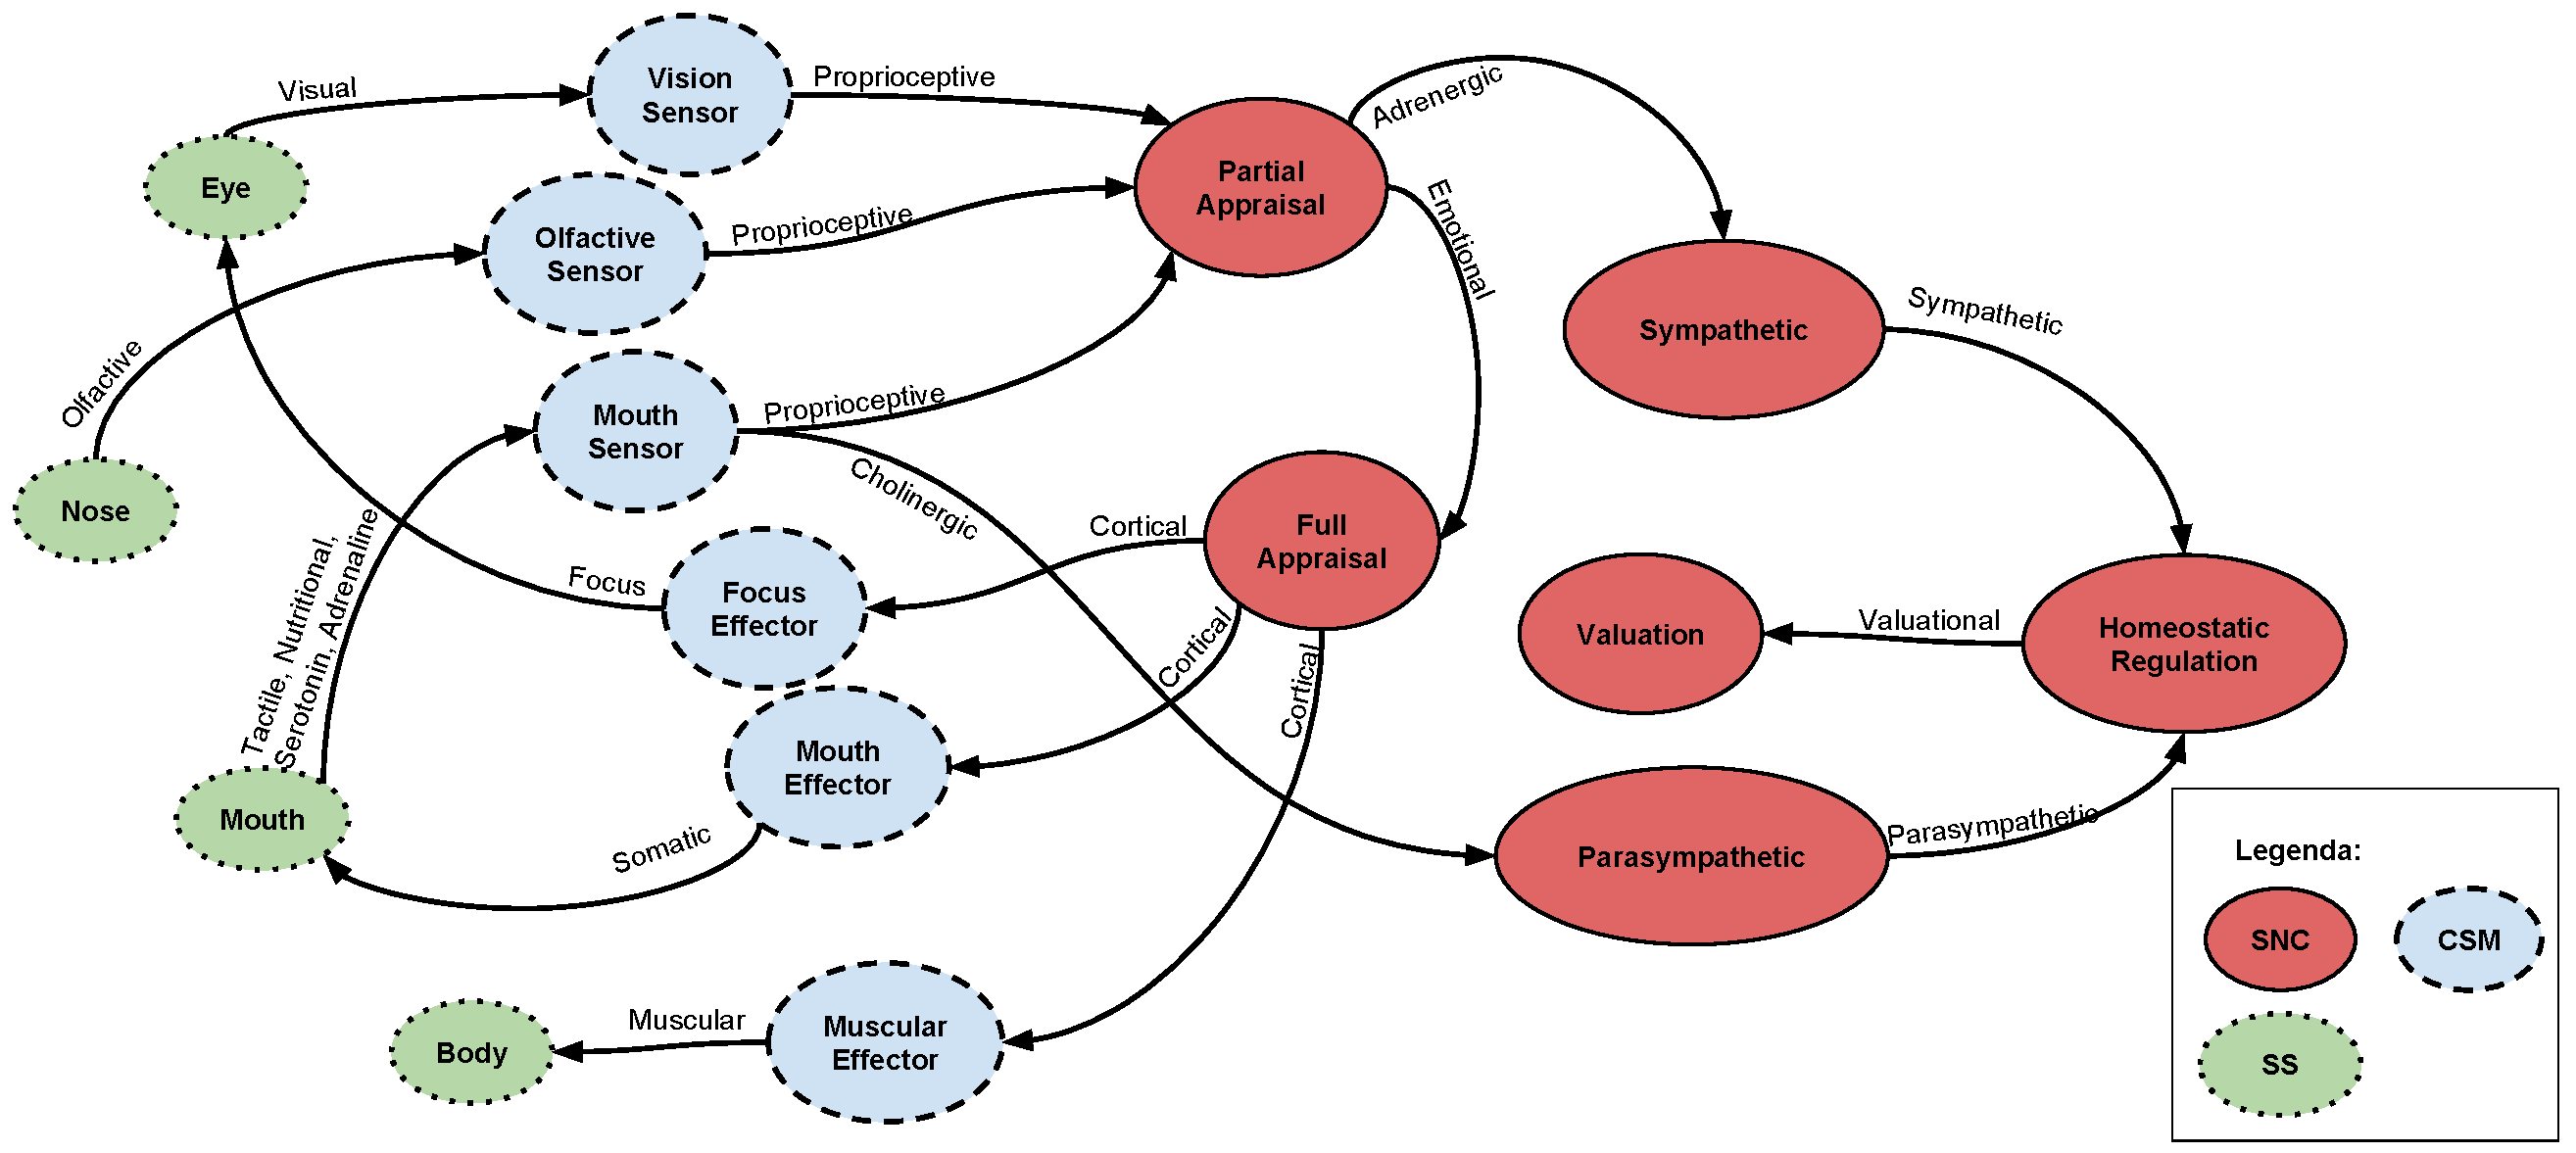
\includegraphics[angle=90,scale=0.5]{./04-figuras/Fig1_CadeiaEstimulos}
    \fonte{O próprio autor}
    \label{fig:cadeiaEstimulos}
\end{figure}

Alguns componentes precisam esperar um certo conjunto de estímulos para funcionar, \textit{e.g.} os que integram o córtex sensório-motor, só podem enviar estímulos ao sistema nervoso central uma vez que o sistema somático tenha informado haver algum objeto no campo sensório da criatura. Componentes do SNC por sua vez não precisam aguardar estímulos o tempo todo, que é o caso do \textbf{PartialAppraisal} que faz a avaliação emocional.  A \autoref{fig:cadeiaEstimulos} exibe a cadeia de estímulos trocados entre os componentes internos da criatura artificial. 

A criatura interage com o mundo artificial, através dos seus componentes do sistema somático, a fim de manter a sua regulação homeostática, \textit{i.e.}, manter o nível de excitação de suas emoções em um  valor estável. Para ilustrar o funcionamento da dinâmica interna, será oferecida uma descrição hipotética da sequência de eventos que acontecem quando um objeto entra em seu campo de visão. A descrição abaixo apresentada foi inspirada na proposta por \citeonline{Campos2015} e serve apenas para fim explicativo uma vez que a troca de estímulos é assíncrona e não determinística. Com isso em mente, supondo que a criatura está caminhando pelo mundo quando dois nutrientes A e B entram em seu campo de visão, e olfativo, ambos em contato com a sua boca: 

\begin{enumerate}
    \item o componente \textbf{Eye} receberá dois estímulos do tipo \textbf{Luminous}, um para cada nutriente. E enviará, para cada um deles, um estímulo do tipo \textbf{Visual} para o\textbf{ VisionSensor};
    \item O componente \textbf{Nose} receberá, concorrentemente um estímulo do tipo \textbf{Smell} para cada nutriente, e enviará para o \textbf{OlfactiveSensor} dois estímulos do tipo \textbf{Olfactive};
    \item o componente \textbf{Mouth} receberá dois estímulos do tipo \textbf{Mechanical} e enviará dois estímulos do tipo \textbf{Tactile} ao \textbf{MouthSensor}; 
    \item Os componentes sensores (\textbf{MouthSensor}, \textbf{VisionSensor} e \textbf{OlfactiveSensor}) ao receberem os estímulos citados, produzirão para cada um deles um estímulo do tipo \textbf{Proprioceptive}, que será enviado ao \textbf{PartialAppraisal}, esses estímulos podem chegar juntos ao componente \textbf{PartialAppraisal} ou não;
    \item Supondo que o \textbf{PartialAppraisal} recebe todos os seis estímulos proprioceptivos, ele criará uma situação, que representa o conjunto de sensores ativados e por quais componentes. Essa situação será enviada juntamente com a emoção mais desregulada ao componente \textbf{FullAppraisal}. Supondo que essa emoção seja a fome, ela será utilizada para calcular a eficiência comportamental da criatura. O \textbf{PartialAppraisal} também envia um estímulo do tipo \textbf{Adrenergic} ao componente \textbf{Sympathetic}, dizendo que o \textit{arousal} das emoções deve ser atualizado;
    \item O componente \textbf{Sympathetic} envia um estímulo ao \textbf{HomeostaticRegulation} para atualizar o \textit{arousal} de todas emoções, somando uma constante que será chamada de delta simpático $ \Delta_{sym} $;
    \item o \textbf{FullAppraisal}, ao receber o estímulo do tipo \textbf{Emotional}, criará uma lista de possibilidades de ações, ou \textit{affordances}, que no caso são: comer o nutriente A, comer o nutriente B, evitar os nutrientes, andar em qualquer direção ou dormir. Essa lista, juntamente com a emoção mais desregulada, será enviada ao AS para escolher a próxima ação a ser executada que melhor regula a emoção fome. O AS utiliza os sistemas condicionamento e memória para desambiguar o conjunto de ações, caso não seja possível ele escolhe uma ação aleatória do conjunto de \textit{affordances}.  Assumindo que a ação de comer o nutriente A será escolhida, o \textbf{FullAppraisal} envia para os componentes do córtex efetor  (\textbf{FocusEffector}, \textbf{MouthEffector} e \textbf{MuscularEffector}) em um estímulo cortical essa informação;
    \item O estímulo cortical recebido no \textbf{MouthEffector} é transmitido ao componente \textbf{Mouth} por uma mensagem do tipo \textbf{Somatic} e ao ser recebida no orgão efetor, desencadeia um estímulo destrutivo ao nutriente A;
    \item Os outros componentes do córtex efetor atualizam, nos seus respectivos membros do sistema somático, o valor da eficiência comportamental, que é utilizada para calcular os parâmetros de sensibilidade (dimensão do campo visual, olfativo, tamanho do passo, etc.);
    \item Ao receber uma mensagem destrutiva, o nutriente se remove do mundo e envia à criatura que o destruiu um estímulo nutritivo;
    \item O componente \textbf{Mouth}, recebendo o estímulo nutritivo envia um estímulo do tipo \textbf{Nutritional} para o \textbf{MouthSensor};
    \item O sensor, ao receber o estimulo nutricional, envia ao \textbf{Parasympathetic} um estímulo \textbf{Cholinergic};
    \item O estímulo \textbf{Cholinergic} é recebido no \textbf{Parasympathetic} que encaminha ao \textbf{HomeostaticRegulation} informando que o \textit{arousal} da emoção fome deve ser diminuído. Essa diminuição é igual ao valor nutritivo do estímulo recebido;
    \item O \textbf{HomeostaticRegulation} envia uma mensagem ao \textbf{Valuation} informando que o nutriente já foi comido e a emoção já regulada, e a ação que produziu essa regulação deve ser valorada;
    \item O \textbf{Valuation} atualiza a memória de condicionamento e a memória de longo prazo ao receber uma mensagem do \textbf{HomeostaticRegulation} e o ciclo de estimulação termina neste passo.
\end{enumerate}

É importante ressaltar que o processamento dos estímulos acontece de  maneira concorrente,  e essa é só uma das possíveis ordens de execução. Ademais, o início de um novo ciclo em algum outro componente não influencia o que já está em execução, podendo produzir comportamentos distintos.

Dada a organização entre os componentes da criatura, a estratégia escolhida  para implementá-la  foi criar um ator tipado\footnote{Atores em Akka podem ser não tipados (como nos exemplos do capítulo anterior) ou tipados. Atores tipados devem implementar alguma interface e são acessíveis através e somente dela, como objetos convencionais, mas com as mesmas propriedades de atores convencionais. Para maiores detalhes de implementação, a documentação se encontra em \url{http://doc.akka.io/docs/akka/current/scala/typed-actors.html}} cujo sub-atores criados são seus componentes internos. A hierarquia dos objetos é de um único nível, de forma a facilitar a um componente acessar a referência para outro componente. 

Como os atores de Akka tratam uma única mensagem por vez e o modelo de sistema nervoso do Artífice prevê que um componente deve ser capaz de tratar mais de um estímulo ao mesmo tempo, foi necessário estender a \textit{mailbox default} do \textit{toolkit}, mudando o seu comportamento ao desenfileirar. Na nova implementação, ao ser solicitada a próxima mensagem, o método empacota todas as mensagens que estão na fila em uma lista e entrega essa lista ao ator. Esse novo comportamento cria uma dificuldade ao ator destinatário, que não saberá a referência do remetente de cada mensagem a partir do método \textbf{sender()}, uma vez que os estímulos são desempacotados de seus envelopes que contém essa informação, e empacotados em um novo envelope sem remetente. Entretanto, todo estímulo enviado possui dois identificadores do tipo \textbf{SequentialId} que mantêm o \textit{id} do remetente e do destinatário. Para recuperar o ator que enviou a mensagem, o ator da criatura, que supervisiona os componentes, mantêm uma tabela \textit{hash} que mapeia \textbf{SequentialId}s para o \textbf{ActorRef} do componente.

O \textbf{PartialAppraisal} é um tipo especial de componente, que  precisa exibir um comportamento ativo, enviando estímulos ainda que não tenha recebido nenhum. Como os atores de Akka são reativos, no sentido de que só são executados ao receber uma mensagem de outro ator, é necessário utilizar algum artifício que faça o \textbf{PartialAppraisal} executar periodicamente. Para foi criada uma tarefa no \textit{scheduler} de cada criatura que envia uma uma mensagem para o componente periodicamente. Assim, ainda que não haja nenhuma mensagem vinda do córtex sensor o componente será escalonado de tempos em tempos para tratar, ao menos, essa mensagem. 

Por fim, um ponto importante da implementação das criaturas artificiais é a comunicação com o banco de dados. Ela deve acontecer sempre que um componente terminar sua execução, persistindo dados importantes para analise posterior. Esses dados em geral são o estado de cada componente, o conjunto de estímulos que ele recebeu e que alterou seu estado interno, e o conjunto de estímulos que ele emitiu ao alterar esse estado. A tecnologia utilizada para criar as tabelas do banco de dados e fazer o acesso durante a simulação foi a \textit{Java Persistence API} (JPA). Ela foi escolhida para manter compatibilidade com versões anteriores da arquitetura Artífice. 

O diagrama de classes que são persistidas em banco de dados está representado na \autoref{fig:bd}. É possível ver na figura que todos os objetos que representam algum estado relevante durante a simulação estão associados a um \textbf{ChangeStimulusState}. Esta entidade de banco de dados é de grande importância pois é responsável por manter as transduções de estímulos. A saber, uma transdução é a transformação de estímulo que recebido em um estímulo emitido, produzindo uma mudança de estado interno em um componente. Toda alteração de estado é salva com o \textit{timestamp} em que ela aconteceu e, juntamente com a entidade \textbf{StimulusState}, forma um grafo pelo qual é possível reconstruir a cadeia de estimulação que produziu um comportamento qualquer da criatura artificial. 

É relevante  saber o instante em que os componentes alteraram seu estado uma vez que este modelo cognitivo se comporta como um sistema dinâmico no tempo, e a maioria das análises são feitas baseadas nele. Além disto, como este é um sistema inteligente que deve exibir um comportamento coerente, é necessário também correlacionar a dinâmica externa da criatura artificial com seu estado interno. A título de exemplo, é preciso saber se a criatura come quando sua emoção mais desregulada é a fome, ou qual mecanismo de decisão ele usa para desambiguar uma ação.  

\begin{comment}
 -- timestamp em  tudo, como é um sistema assincrono
 -- um sistema com um grau de inteligencia é necessário correlacionar os dados da dinamica interna e externa 
 -- retirar as informações necessarias pra reconstruir grafico da dinamica interna e externa
 -- dar um exemplo, queremos saber se estando com fome ele opta por decidir comer algo ou fazer outra 
\end{comment}

\begin{figure}
    \centering
    \caption{Diagrama de classes do banco de dados}
    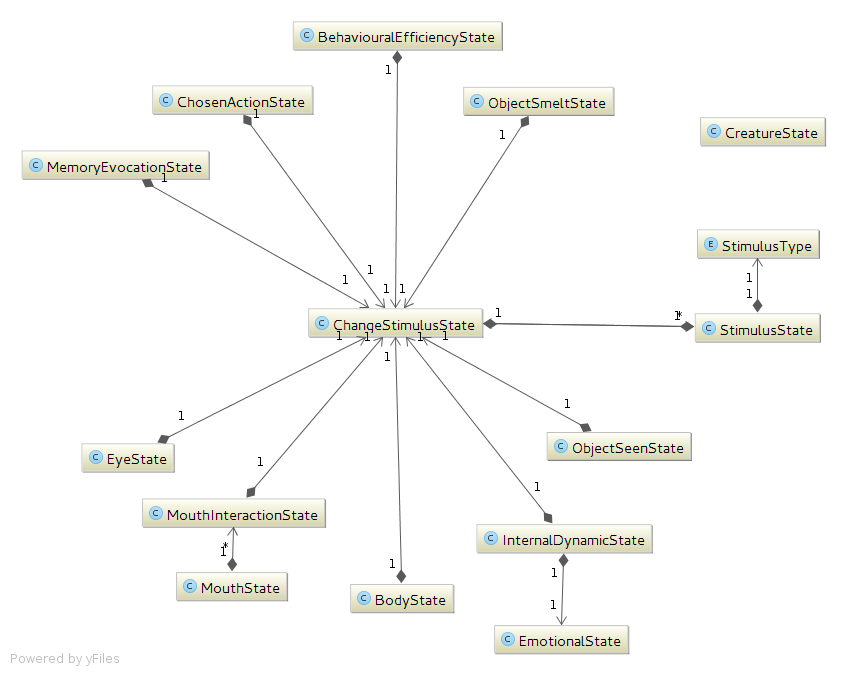
\includegraphics[scale=0.55]{04-figuras/bd.png}
    \fonte{O próprio autor}
    \label{fig:bd}
\end{figure}

\section{Dos componentes da simulação em ambiente distribuído}
\label{sec:cluster}

Ao particionar o funcionamento da arquitetura Artífice, foram identificados quatro papéis importantes que podem funcionar de modo distribuído, eles são: o gerenciamento da simulação; gerenciamento dos componentes da simulação (criaturas e nutrientes); o fornecimento de identificadores, e a manutenção física da simulação. Para cada uma das responsabilidades apresentadas foram projetados um ator e suas peculiaridades serão descritas adiante. A \autoref{fig:cluster} mostra um esquema de como os atores se organizariam com $K$ \textit{holders}, $M$ criaturas e $N$ nutrientes. Este esquema é um dos muitos possíveis que poderiam ser adotados e foi escolhido tendo em vista o balanceamento de criaturas e nutrientes ao longo dos nós de processamento, entretanto, outras possibilidades de organização devem ser estudadas em trabalhos futuros, analisando a performance em termos de sistemas distribuídos, bem como a mudança desse esquema de distribuição influencia o comportamento das criaturas.

\begin{figure}
    \centering
    \caption{Esquema de nós do \texit{cluster}. Os atores conectados por linhas pontilhadas podem executar em máquinas separadas enquanto os atores conectados por linhas contínuas estão subordinados, devendo executar no mesmo computador que seus supervisores. As linhas pontilhadas portanto indicam que a comunicação acontece via rede, enquanto as linhas contínuas indicam que a comunicação acontece sem o uso da rede}
    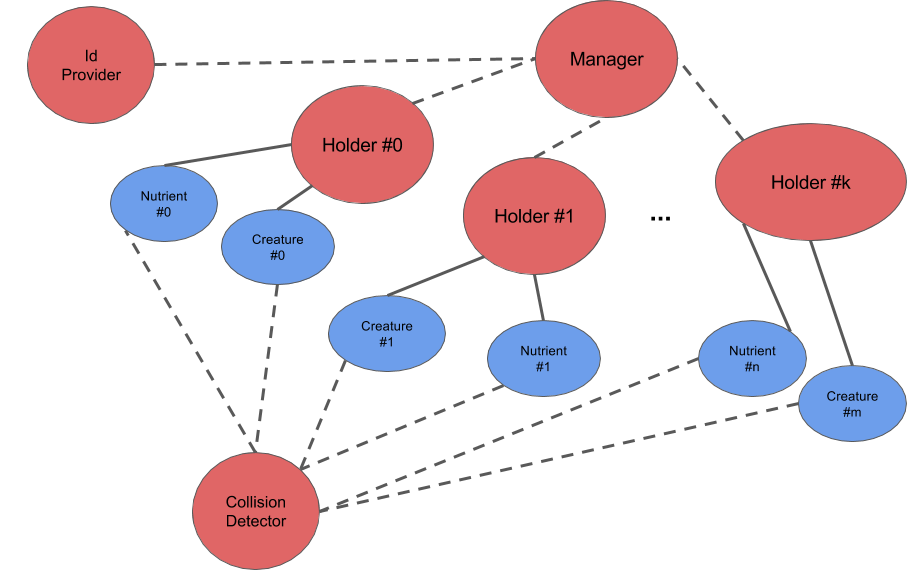
\includegraphics[scale=0.5]{04-figuras/cluster.png}
    \fonte{O próprio autor}
    \label{fig:cluster}
\end{figure}

Para auxiliar na comunicação de atores em diferentes processos foi utilizada a biblioteca \textit{akka-cluster} \footnote{\url{http://doc.akka.io/docs/akka/current/java/common/cluster.html}} que faz parte do \textit{toolkit} Akka. Ela oferece um serviço descentralizado de adesão de atores, distribuídos em vários processos ao longo da rede. A biblioteca permite identificar quando novos membros entram na rede ou saem dela. Ela é baseada no protocolo \textit{gossip} e possui um detector automático de falhas, oferecendo um serviço sem ponto único de falha ou ponto único de gargalo.

O ator responsável pelo gerenciamento da simulação, o \textit{manager}, tem o papel de iniciar e interromper a simulação, fazendo interface com o usuário final. Ele mantém uma tabela com a referência de todos os nós associados a uma simulação, e é responsável por entregar um identificador a todo novo nó  do tipo \textit{holder} que entra no \textit{cluster}. Esse identificador será necessário para encontrar de forma eficiente um membro da simulação em um nó do \textit{cluster} partindo de outro nó qualquer. Ao receber uma notificação que um nó importante falhou, a simulação é imediatamente interrompida pelo \textit{manager}. 

Como os identificadores do tipo \textbf{SequentialId} são globais para toda a simulação, optou-se por gerá-los de forma centralizada, garantindo que não existam dois identificadores repetidos. Essa estratégia foi adotada por ser a que teria menor \textit{overhead} de implementação. Tratar a falha do \textit{id-provider}, ator responsável por gerar os identificadores, é simples de corrigir: reinicia-se o ator em outro nó. O \textit{manager} deve ter conhecimento do \textit{id-provider} mas não é necessário mantê-lo indexado.

As colisões entre os objetos da simulação continua sendo verificada por um nó centralizado chamado \textit{Collision Detector}. Esse nó recebe mensagens constantemente, sempre que uma criatura atualiza sua posição ou um nutriente é destruído, e deve responder, a cada nova mensagem, com quais objetos o remetente colidiu. O algoritmo de pesquisa que encontra o conjunto de objetos com o qual o remetente da mensagem colidiu é sequencial e linear no número de objetos no mundo, o que pode ser um gargalo, à medida que o tamanho do mundo cresce. Esta tarefa é de crucial importância para um AD-MAS como este em que, o mundo artificial possui uma representação geométrica e toda a dinâmica de interação entre as criaturas e objetos depende desta representação. Dessa forma, manter a verificação de colisões centralizada em um nó, além de caracterizar um ponto único de falha (o que é um aspecto negativo do ponto de vista de sistemas distribuídos), pode ser prejudicial para o desempenho e escalabilidade, além de levar dinâmica interna das criaturas à degradação. Neste sentido, é importante reforçar a necessidade de avaliar outros modelos de distribuição, levando em conta uma melhor abordagem para o problema de verificar colisões em um sistema distribuído que depende do tempo.  

Finalmente, o \textit{holder} é responsável por manter as entidades da simulação, criaturas e nutrientes. Ele também mantém uma tabela com os outros \textit{holders} que fazem parte do \textit{cluster}. Esse índice é construído dinamicamente à medida em que as criaturas vão trocando estímulos com os objetos do mundo que podem estar em outros \textit{holders}. Ao entrar no \textit{cluster}, um \textit{holder} deve receber um identificador inteiro sequencial do \textit{manager}. Ao receber a informação do usuário que um novo membro deve ser criado, é papel do \textit{manager} solicitar um novo \textbf{SequentialId} ao \textit{id-provider}. O resto da divisão inteira da super-chave do identificador pelo número de \textit{holders} no \textit{cluster} informa em qual \textit{holder} o novo membro deve ser criado. Assim o \textit{manager} ordena a criação do novo membro no nó apropriado. 

As criaturas dentro de um \textit{holder} podem eventualmente querer se comunicar com membros em outro \textit{holder} a partir dos identificadores trocados nas mensagens, sem saber exatamente onde está fisicamente o ator, \textit{e.g.} uma criatura que está no \textit{holder-1} pode querer enviar um estímulo destrutivo para um nutriente que esteja no \textit{holder-2}. Para tanto, a criatura encaminha a mensagem ao seu \textit{holder}: caso ele conheça o nó do destinatário, a mensagem é encaminhada a ele. Caso o \textit{holder} do destinatário seja desconhecido, a mensagem é enviada ao \textit{manager} que a encaminha ao \textit{holder} apropriado e responde com o endereço dele ao \textit{holder} remetente, para  que ele seja indexado. Esse algoritmo é baseado no \textit{plugin} \textit{akka-cluster-sharding}, que oferece a funcionalidade de endereçar um ator por um identificador lógico sem conhecer sua localização física. Optou-se por adotar uma versão simplificada do algoritmo em detrimento do \textit{plugin} uma vez que o segundo permite a migração de entidades entre nós do cluster, o que não é uma funcionalidade desejável para a simulação de vida artificial proposta, pois não se sabe o impacto que a transição de um nó para outro pode causar a dinâmica interna da criatura artificial.

\section{Considerações finais}

Até aqui foi apresentada uma proposta de de modelagem e implementação de um simulador de criaturas artificiais, dotadas de um sistema nervoso artificial que se comporta como um AD-MAS. Os sistemas e sub-sistemas da criatura foram descritos, bem como os componentes desses subsistemas e suas interações, todas baseadas em comunicação assíncrona. Há também uma proposta de organização dos atores em um \textit{cluster}. 

Em especial o modelo do sistema nervoso implementado é equivalente ao da arquitetura Artífice. A escolha por ele se dá pela sua diversidade de fontes, não sendo baseado em uma única teoria cognitiva, mas sim num arcabouço de várias teorias de diferentes áreas, da biologia, psicologia à neurociências. Para além disso, os princípios do modelo de atores entram em íntima conformidade com os adotados na modelagem do sistema nervoso.

Espera-se com este sistema ser possível executar simulações de forrageamento, onde uma criatura que vive em um mundo artificial, em que há variedade de alimento, aprenda a escolher quais alimentos são melhores e quando é o melhor momento para tomar a decisão de comer uma presa.

Espera-se também que seja possível executar essas simulações com um número grande de criaturas e máquinas, até o limite imposto pela tecnologia e solução proposta. Um conjunto de experimentos preliminares está descrito no próximo capítulo, e seus objetos são exatamente entender o comportamento do software produzido e vislumbrar as limitações desta solução. 			% Metodologia
% -----------------------------------------------------------------------------
%   Arquivo: ./02-elementos-textuais/resultados.tex
% -----------------------------------------------------------------------------

\begin{comment}

-- escrever um esquema dos experimentos que devem ser executados

-- separar em seções, uma pra cada experimento, apresentar o experimento, o resultado, e discutir

-- mostrar se o mecanismo funciona exatamente como esperado, para uma única criatura, as duas implementação são qualitativamente comparáveis 

-- estudar mais de uma criatura, mostrando que uma tem comportamento similar a outra, 


-- ARREFECIDA
\end{comment}


\chapter{Análise e Discussão dos Resultados}
\label{chap:resultados}
Apresentada no capítulo \autoref{chap:metodologia} a modelagem de um simulador de criaturas artificiais assíncrono e distribuído, baseado no arquitetura Artífice, é necessário validar dois aspectos do software proposto. Primeiro, no que diz respeito ao comportamento das criaturas artificiais, se ele é qualitativamente comparável com a arquitetura Artífice. O segundo aspecto a se verificar é quão escalável é o sistema, horizontal e verticalmente. Neste sentido, foram propostos três experimentos preliminares, e espera-se que os resultados esclareçam como a nova arquitetura se comporta, em comparação com a primeira, tal como na presença de várias criaturas em uma mesma máquina, e distribuída em vários nós diferentes.

Estes experimentos foram realizados no \textit{cluster} do Laboratório de Sistemas Inteligentes (LSI) do CEFET, composto de oito máquinas com processador Intel i7, 32GB de RAM e 2TB de HD cada. O sistema operacional utilizado é o CentOS 6, e o SLURM como escalonador de tarefas. Cada experimento foi executado 30 vezes. Esse número de repetições foi escolhido de modo que os valores de erros relativo às médias esteja próximo à 10\%.

Os dados considerados relevantes para a análise da dinâmica externa das criaturas artificiais são o de tempo de vida, a distância percorrida e a quantidade de nutrientes comidos. Dos resultados da dinâmica interna é importante analisar três medidas ao longo do tempo, a saber: a quantidade de estímulos trocados, a utilização dos mecanismos de aprendizagem e seleção de ação e a quantidade de presas ingeridas. A primeira delas é relevante para verificar se todos os estímulos estão sendo corretamente enviados e recebidos, e se a taxa com que eles são trocados é coerente. O segundo e terceiro aspecto dizem da adaptação e do correto funcionamento dos mecanismos de aprendizagem, se as escolhas que a criatura faz (e como ela as faz) guarda correlação com sua história de interações passadas. Dito de outro modo, é necessário saber se a criatura aprende que comer uma presa sem valor nutricional não vale a pena, que dormir quando está com fome também não vale a pena e que comer uma presa de maior valor nutricional é melhor que comer um de menor valor. 

Como descrito no capitulo anterior, os dados da simulação são gravados em banco de dados relacional, e para todo evento é mantido o \textit{timestamp} (em milisegundos) em que ele aconteceu. Como se trata de uma simulação de um sistema dinâmico, cujo estado evolui no tempo, é necessário calcular as médias temporais para cada um dos parâmetros mencionados acima, que descrevem o sistema. Para tanto, os eventos são ordenados e agrupados pelo tempo, convertido em minutos com precisão de três casas decimais. Para cada criatura, em cada instante de tempo, e para cada parâmetro avaliado (\textit{e.g} estímulos trocados, nutrientes comidos, escolhas realizadas) a média aritmética naquele instante é calculada. O erro relativo à média é calculado de acordo com a \autoref{eq:erroRelativo}.

\begin{equation}
 \centering
 ER(X) = Z_{\alpha}\frac{S}{\bar{X}\sqrt{n}}
 \caption{Fórmula para o erro relativo de uma amostra X}
 \label{eq:erroRelativo}
\end{equation}

Onde $X$ é uma das amostras de tamanho $n$ de uma população $P$ de $p$ amostras, $\bar{X}$ é a média amostral, $S$ é o desvio padrão amostral e $Z_{\alpha}$ é a constante para um intervalo confiança de 95\%. O erro relativo $ER(X)$ é dado em percentual e vale como uma medida da qualidade da média da amostra $X$. 

Desta feita, a próxima seção apresenta os resultados de validação do modelo, contrapondo com os resultados da arquitetura Artífice para configuração semelhante. A \autoref{sec:esc_vertical} apresenta o experimento feito em uma única máquina para verificar a escalabilidade vertical do software. A \autoref{sec:esc_horizontal} apresenta os resultados do experimento executado com mais de uma máquina a fim de verificar a escalabilidade horizontal. 
Os resultados são discutidos na \autoref{sec:sintese} que encerra este capitulo.

\section{Validação do modelo}
\label{sec:validacao}
Este experimento foi realizado para verificar a compatibilidade do comportamento das criaturas entre a arquitetura Artífice e a DL2L. Foi executada uma simulação de forrageamento (busca por alimento) com uma única criatura em cada arquitetura e 50 presas de três tipos diferentes totalizando 150 nutrientes, que são: maçãs vermelhas (RA), maçãs verdes (GA), e maçãs cinzas (GRA). O valor nutricional $N$ em ambos os experimentos respeita a relação $N_{GRA} = 0 < N_{RA} < N_{GA} $. Cada experimento foi repetido por 30 vezes. A arquitetura Artífice foi configurada com um $\Delta_{sym} = 3 \times 10^{-3}$, enquanto a arquitetura DL2L foi configurada com um $\Delta_{sym} = 1.5 \times 10^{-3}$. Esses parâmetros foram escolhidos de forma que as criaturas pudessem interagir com o mundo artificial por um tempo aceitável, sendo possível observar o seu comportamento. Os gráficos da evolução do erro para ambas as arquiteturas estão apresentados na \autoref{ap:erroExp1}.

Para a configuração descrita a arquitetura Artífice obteve um tempo de vida médio de $12.6 \pm 9.96\%$ em minutos e comeu um número de $25.3 \pm 10\%$ presas. O teste de normalidade para o tempo de vida e presas comidas resultou em p-valores de $1.4\%$ e $3.7\%$ respectivamente, valores que não permitem dizer que a distribuição é normal. Já a arquitetura DL2L obteve nesse experimento um tempo de vida médio de $31.4 \pm 6.79\%$ em minutos e comeu, em média, $304.2 \pm 4.35\%$ presas. O teste de normalidade para o tempo de vida e presas comidas resultou em p-valores de $48.07\%$ e $65.72\%$, o que indica que as distribuições são normais para um intervalo de confiança de $95\%$.

A média temporal da troca de estímulos entre as arquiteturas está apresentada na \autoref{fig:exchgStimuli}. Vale dizer que a arquitetura DL2L tem um número menor de tipos de estímulos comparada à Artífice, e isso se deve a uma simplificação dos componentes e do fato de que nem todas as funcionalidades foram implementadas por completo, somente as mais críticas para o funcionamento do sistema nervoso e do processo cognitivo. A título de exemplo, o mecanismo de reprodução, proposto por \citeonline{Assis2013}, não foi implementado nesta primeira versão da DL2L.

\begin{figure}[h!]
    \centering
    \caption{Média da troca de estímulos no tempo para ambas as arquiteturas. Cada curva representa um tipo de estímulo diferente. Ambas as médias foram calculadas com precisão de minutos.}
    \begin{subfigure}[b]{1.0\textwidth}
        \caption{Troca de estímulos na arq. Artífice}
        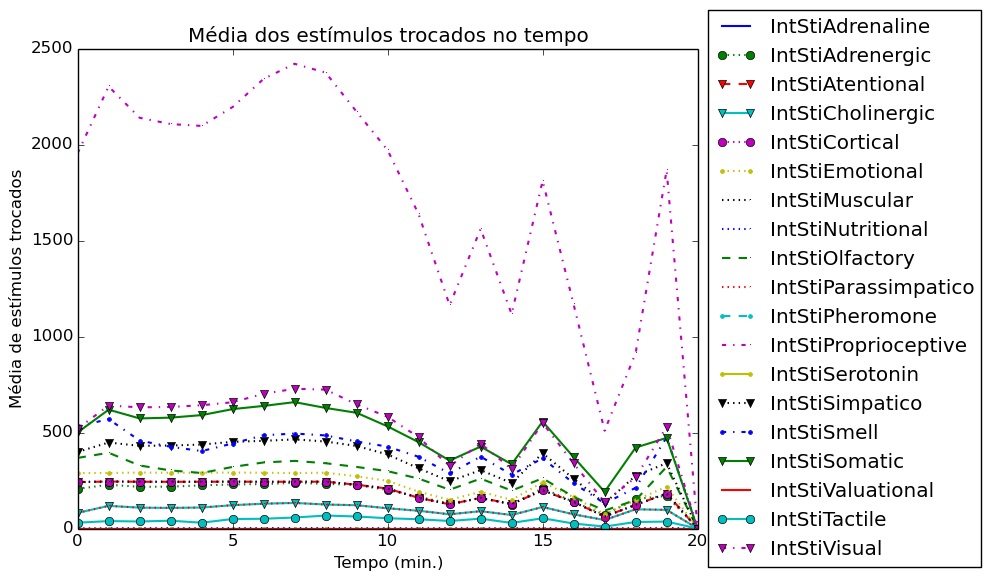
\includegraphics[width=\textwidth]{04-figuras/experiments/exp_1_artifice/avgExchangedStimuliOverTime.png}
        \label{fig:exchgStimuli_artifice}
    \end{subfigure}
    ~
    \begin{subfigure}[b]{1.0\textwidth}
        \caption{Troca de estímulos na arq. DL2L}
        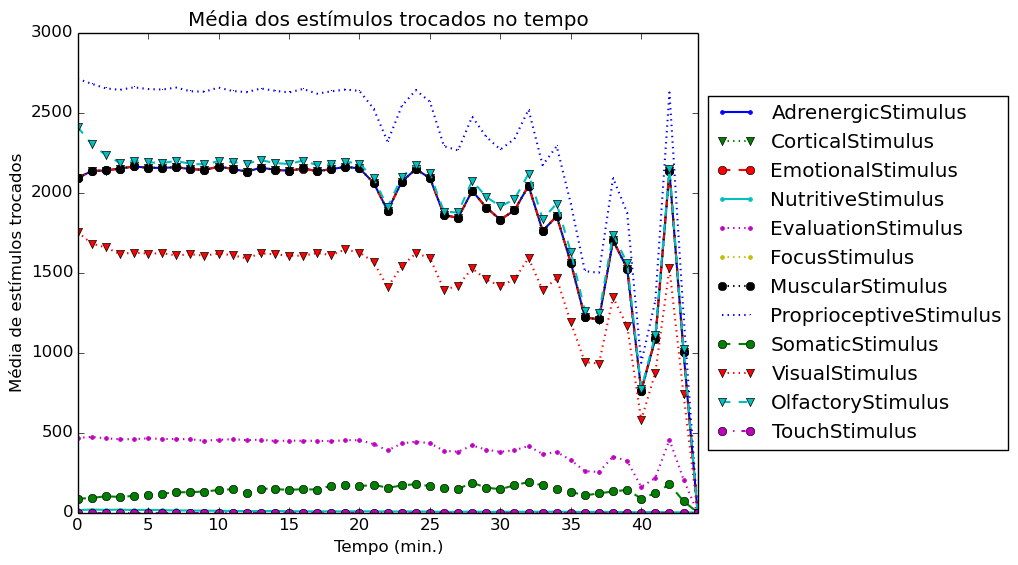
\includegraphics[width=\textwidth]{04-figuras/experiments/exp_1_l2l/avgExchangedStimuliOverTime.png}
        \label{fig:exchgStimuli_dl2l}
    \end{subfigure}
    \label{fig:exchgStimuli}
\end{figure}

A \autoref{fig:accChoices} exibe a média da soma acumulada de escolhas feitas no tempo, separadas por mecanismo. Nesta simulação foram utilizados somente os três mecanismos mais básicos: a criatura seleciona primeiro os alvos que estão à menor distância, depois seleciona a ação mais provável para cada alvo baseado na memória de condicionamento, e por fim, caso não tenha restado uma ação única, ela faz uma escolha aleatória.  

\begin{figure}[h!]
    \centering
    \caption{Gráficos da média de escolhas acumuladas no tempo para a arquitetura Artífice e DL2L}
    \begin{subfigure}[b]{1.0\textwidth}
        \caption{Arquitetura Artífice}
        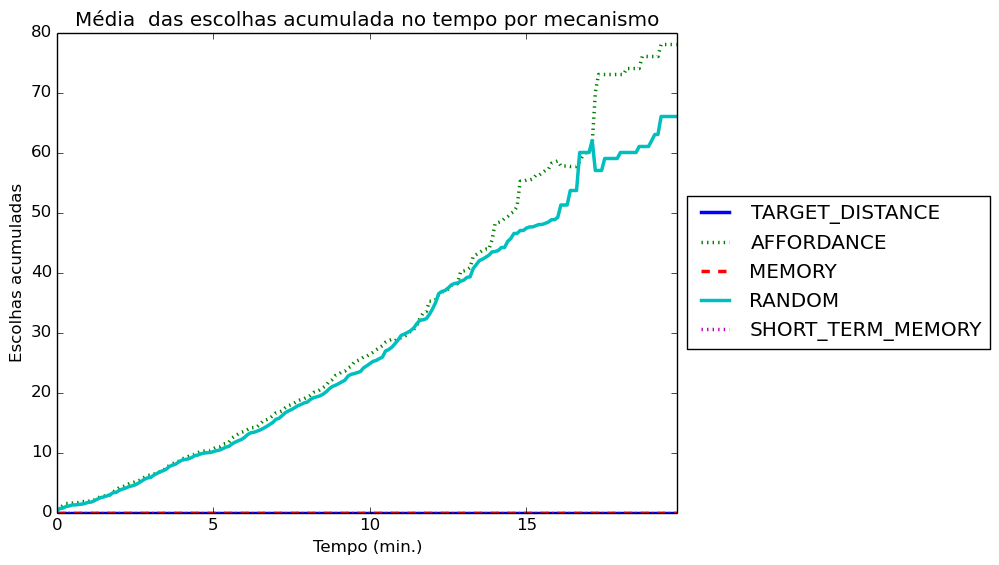
\includegraphics[width=\textwidth]{04-figuras/experiments/exp_1_artifice/accumulatedChoices.png}
        \label{fig:accChoices_artifice}
    \end{subfigure}
    ~
    \begin{subfigure}[b]{1.0\textwidth}
        \caption{Arquitetura DL2L}
        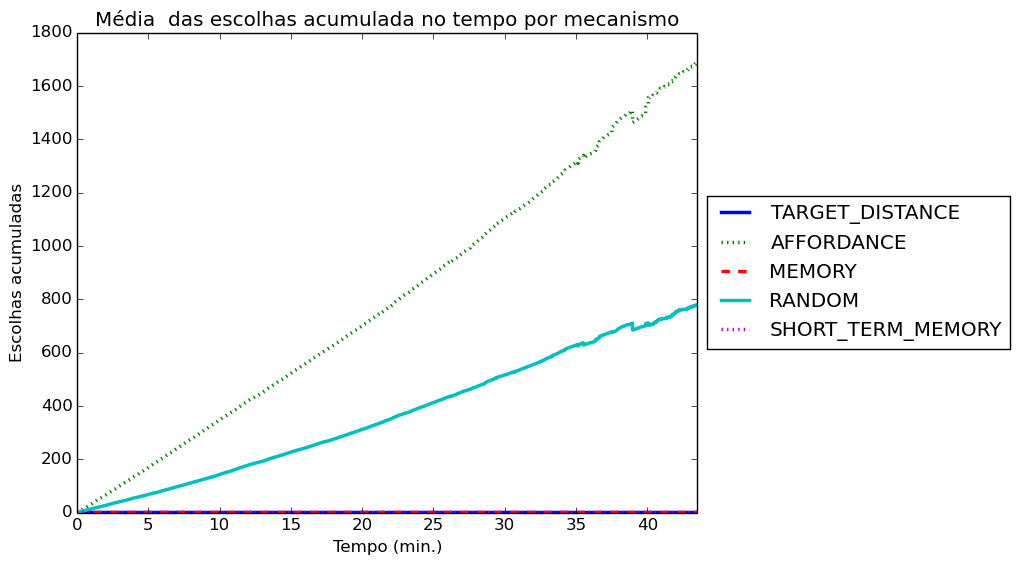
\includegraphics[width=\textwidth]{04-figuras/experiments/exp_1_l2l/accumulatedChoices.png}
        \label{fig:accChoices_dl2l}
    \end{subfigure}
  \label{fig:accChoices}
\end{figure}

A eficiência comportamental da criatura artificial é uma função do máximo \textit{arousal} e da quantidade de objetos no campo sensorial. Ela é calculada durante a execução da simulação e é utilizada para determinar a velocidade do passo da criatura e o foco atencional. Existem duas fórmulas para a eficiência comportamental, uma para tarefas simples onde a decisão envolve um único objeto, e outra para tarefas complexas que envolvem mais de um objeto. A relação da eficiência comportamental em função do \textit{arousal} máximo $A$ e o número de objetos no campo sensor $N$ é apresentada na \autoref{eq:behEfficiency}. A \autoref{fig:behEfficiency} exibe a média temporal normalizada da eficiência comportamental para as duas arquiteturas.

\begin{figure}[H]
    \caption{Cálculo da eficiência comportamental, de acordo com \citeonline{Mapa2009}}
    \[BE(A,N) = 
    \begin{cases}
        5.56A & \text{se } 0 < A < 0.18\\
        16 - 16e^{-0.4A} & \text{se } N < 2\\
        5.714A -  0.816A^2 & \text{se } N \geq 2
    \end{cases}\]
    \label{eq:behEfficiency}
\end{figure}

Para cada tipo diferente de presa a cada instante é calculado quantos nutrientes daquele tipo foram comidos, e a partir dessa série é calculada a soma acumulada. Este dado está apresentado na \autoref{fig:accNutrients} para ambas as arquiteturas.

\begin{figure}
     \centering
    \caption{Gráficos da média da eficiência comportamental no tempo para a arquitetura Artífice e DL2L}
    \begin{subfigure}[b]{1.0\textwidth}
        \caption{Arquitetura Artífice}
        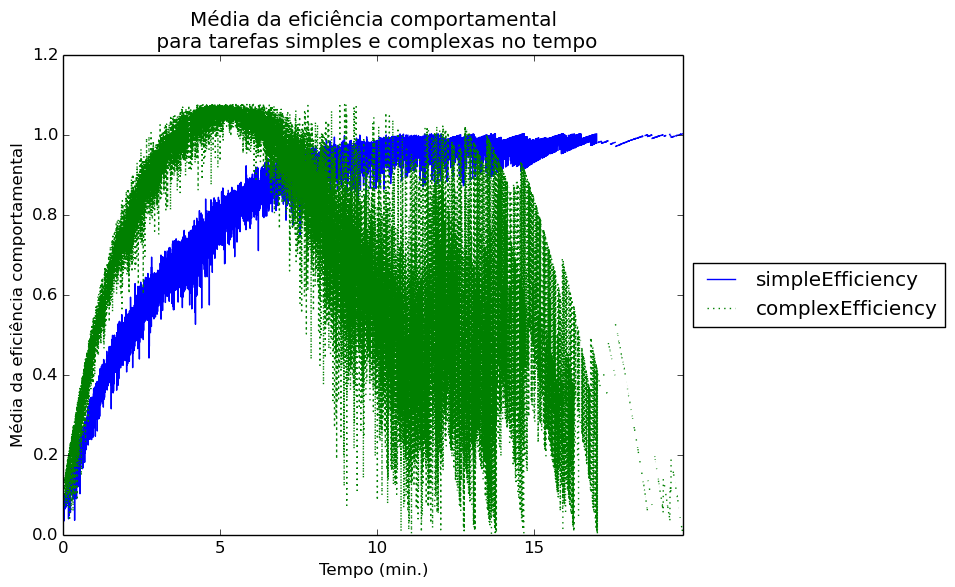
\includegraphics[width=\textwidth]{04-figuras/experiments/exp_1_artifice/behaviouralEfficiency.png}
        \label{fig:behEfficiency_artifice}
    \end{subfigure}
    ~
    \begin{subfigure}[b]{1.0\textwidth}
        \caption{Arquitetura DL2L}
        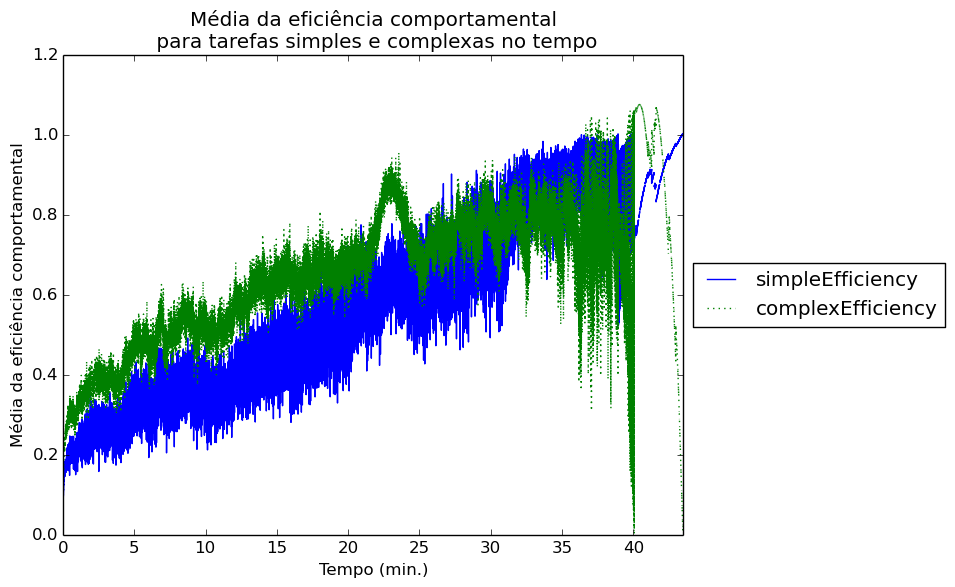
\includegraphics[width=\textwidth]{04-figuras/experiments/exp_1_l2l/behaviouralEfficiency.png}
        \label{fig:behEfficiency_dl2l}
    \end{subfigure}
    \label{fig:behEfficiency}
\end{figure}


\begin{figure}
    \centering
    \caption{Gráficos da média da soma acumulada de nutrientes comidos no tempo}
    \begin{subfigure}[b]{1.0\textwidth}
        \caption{Arquitetura Artífice}
        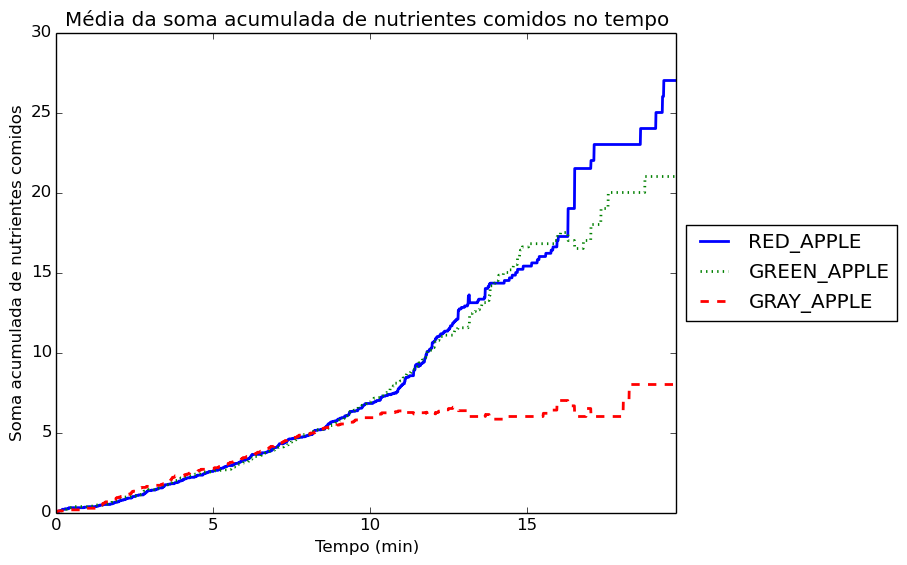
\includegraphics[width=\textwidth]{04-figuras/experiments/exp_1_artifice/accumulatedNutrients.png}
        \label{fig:accNutrients_artifice}
    \end{subfigure}
    ~
    \begin{subfigure}[b]{1.0\textwidth}
        \caption{Arquitetura DL2L}
        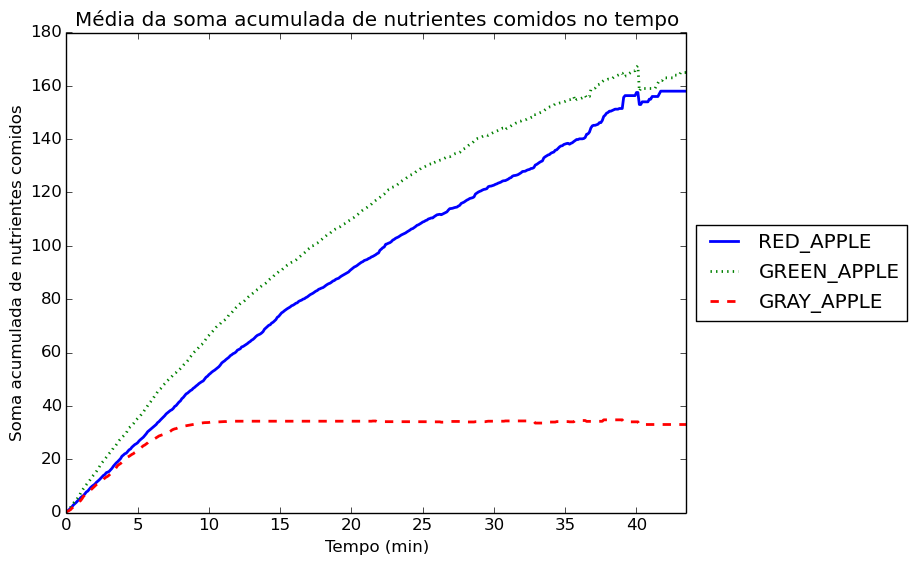
\includegraphics[width=\textwidth]{04-figuras/experiments/exp_1_l2l/accumulatedNutrients.png}
        \label{fig:accNutrients_dl2l}
    \end{subfigure}
    \label{fig:accNutrients}
\end{figure}

\section{Escalabilidade vertical}
\label{sec:esc_vertical}

A fim de verificar a influência de mais de uma criatura em um mesmo \textit{holder} na arquitetura DL2L, este segundo experimento foi proposto.  Foram executadas cinco configurações diferentes, variando o número de criaturas de 1 a 5 mantendo um único nó na simulação. A densidade do mundo é mantida constante entre as configurações, iniciando em 50 presas de cada tipo (assim como no experimento anterior) em um mundo de $4.8 \times 10^{5}$ pixeis. Cada configuração é repetida 30 vezes para garantir um erro relativo próximo a $10\%$. 

A \autoref{tab:resumo_exp2} expõe os resultados da média de tempo de vida, distância percorrida e nutrientes comidos. O erro foi calculado de acordo com a \autoref{eq:erroRelativo}.

\begin{table}[H]
\centering
\caption{Média do tempo de vida, distância percorrida e nutrientes comidos para o experimento 2}
\begin{tabular}{ccccccc}
\hline
\multirow{2}{*}{Criaturas} & \multicolumn{2}{c}{ Tempo de vida } & \multicolumn{2}{c}{ Distância percorrida } & \multicolumn{2}{c}{ Nutrientes comidos } \\
& Média & ER (\%) & Média & ER (\%) & Média & ER (\%) \\
\hline
1 & 31.40 & 6.79 & 2.72E+05 & 9.33 & 304.20 & 4.35 \\
2 & 21.71 & 8.43 & 1.83E+05 & 10.39 & 189.82 & 7.61 \\
3 & 18.81 & 7.24 & 1.30E+05 & 9.90 & 115.38 & 7.79 \\
4 & 13.51 & 6.99 & 9.59E+04 & 9.20 & 62.73 & 8.77 \\
5 & 10.38 & 4.73 & 5.43E+04 & 7.39 & 31.24 & 8.97 \\
\hline
\end{tabular}
\label{tab:resumo_exp2}
\end{table}

Os resultados para a média de estímulos trocados no tempo para cada configuração estão apresentados nas Figuras \ref{fig:exchgStimuli_dl2l}, \ref{fig:exp_2_2_exchgStimuli}, \ref{fig:exp_2_3_exchgStimuli}, \ref{fig:exp_2_4_exchgStimuli} e \ref{fig:exp_2_5_exchgStimuli}. Os gráficos para a evolução do erro relativo no tempo estão apresentados no \autoref{ap:erroExp2}.

\begin{figure}[H]
  \centering
  \caption{Média temporal dos estímulos trocados em simulação utilizando 2 criaturas}
  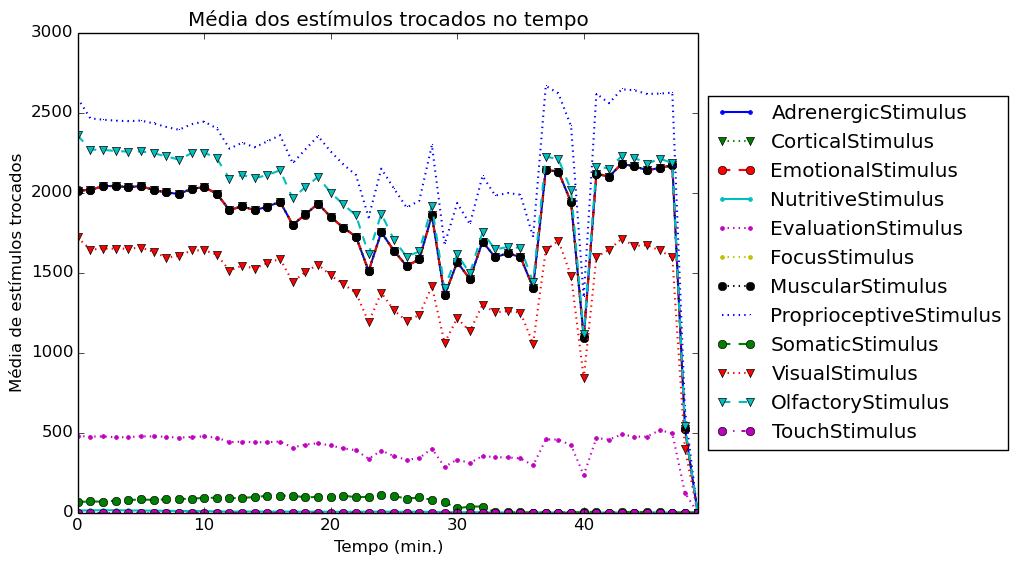
\includegraphics[scale=0.6]{04-figuras/experiments/exp_2/2/avgExchangedStimuliOverTime.png} 
  \label{fig:exp_2_2_exchgStimuli}
\end{figure}

\begin{figure}[H]
  \centering
  \caption{Média temporal dos estímulos trocados em simulação utilizando 3 criaturas}
  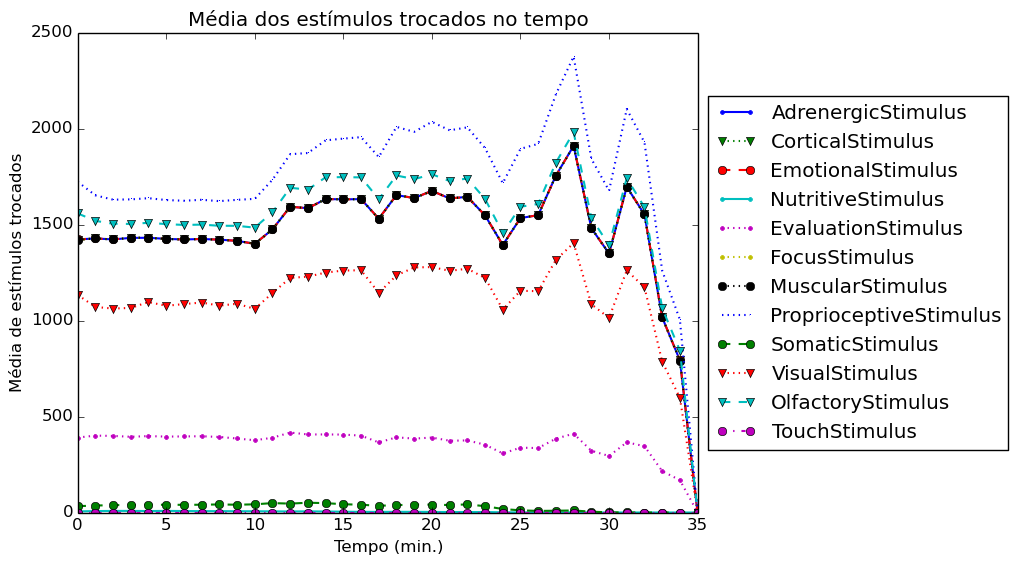
\includegraphics[scale=0.6]{04-figuras/experiments/exp_2/3/avgExchangedStimuliOverTime.png}
  \label{fig:exp_2_3_exchgStimuli}
\end{figure}

\begin{figure}[H]
  \centering
  \caption{Média temporal dos estímulos trocados em simulação utilizando 4 criaturas}
  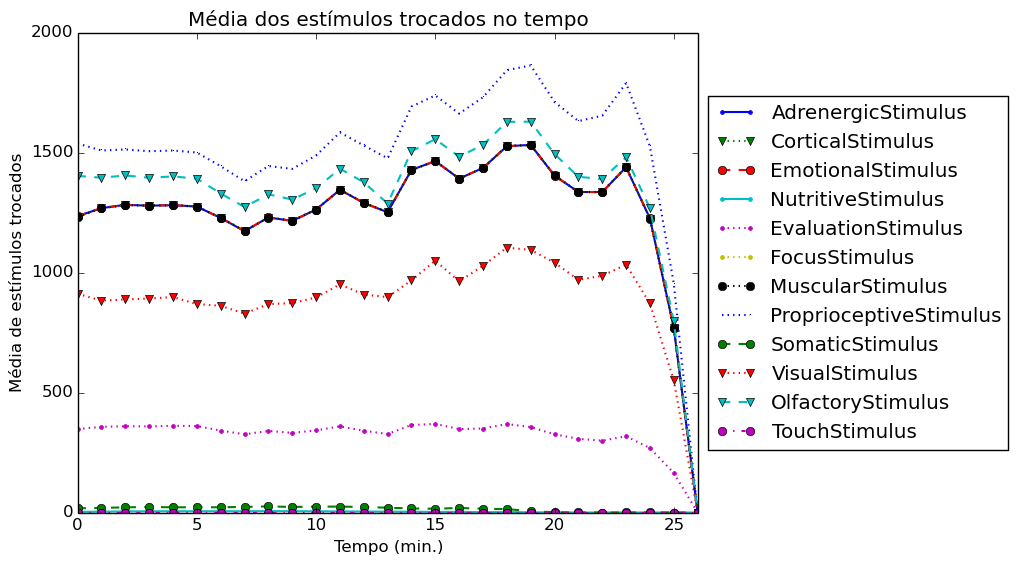
\includegraphics[scale=0.6]{04-figuras/experiments/exp_2/4/avgExchangedStimuliOverTime.png}
  \label{fig:exp_2_4_exchgStimuli}
\end{figure}

\begin{figure}[H]
  \centering
  \caption{Média temporal dos estímulos trocados em simulação utilizando 5 criaturas}
  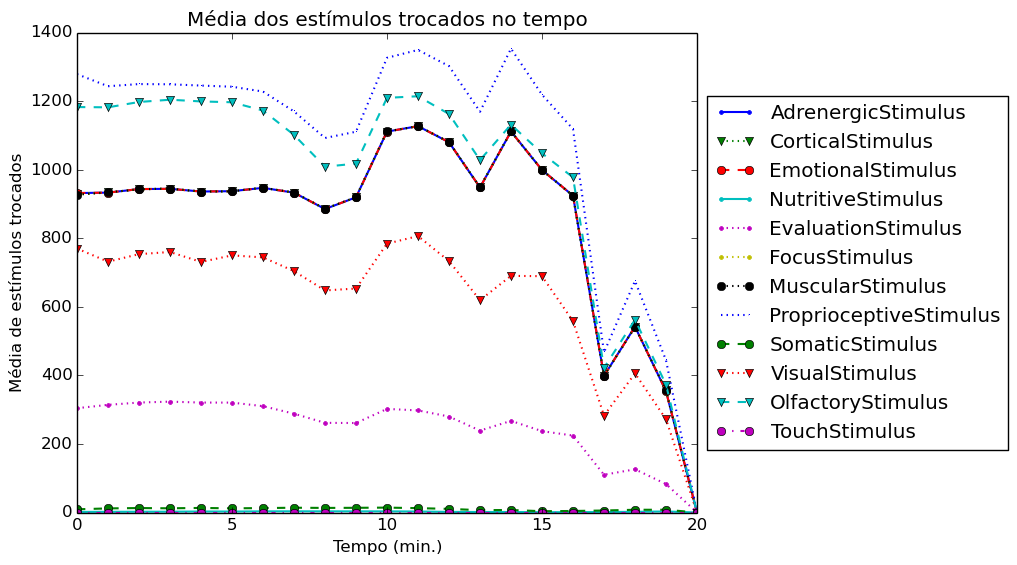
\includegraphics[scale=0.6]{04-figuras/experiments/exp_2/5/avgExchangedStimuliOverTime.png}
  \label{fig:exp_2_5_exchgStimuli}
\end{figure}

A medida que o tempo evolui o erro relativo das médias cresce. Os gráficos de erro estão apresentados na \autoref{ap:erroExp2}.

\section{Escalabilidade horizontal}
\label{sec:esc_horizontal}

Este experimento foi executado com intuito de verificar a influência de mais de um \textit{holder} em uma simulação de forrageamento. Foram executadas cinco configurações diferentes, começando com um \textit{holder} até cinco. Foi mantido o número de uma criatura por nó, e a densidade do mundo foi mantida constante, iniciando com 50 nutrientes de cada tipo em um mundo de $4.8 \times 10^{5}$ pixeis.

Na \autoref{tab:resumo_exp3} estão apresentados os resultados da média de tempo de vida, distância percorrida e nutrientes comidos. O erro foi calculado de acordo com a \autoref{eq:erroRelativo}. É notável que a medida que o número de holders aumenta, há uma diminuiçao em todas as médias. 

\begin{table}[H]
\centering
\caption{Média do tempo de vida, distância percorrida e nutrientes comidos para o experimento 3}
\begin{tabular}{ccccccc}
\hline
\multirow{2}{*}{Criaturas} & \multicolumn{2}{c}{ Tempo de vida (min.) } & \multicolumn{2}{c}{ Distância percorrida } & \multicolumn{2}{c}{ Nutrientes comidos } \\
& Média & Erro (\%) & Média & Erro (\%) & Média & Erro (\%) \\
\hline
1 & 31.40 & 6.79 & 2.72E+05 & 9.33 & 304.20 & 4.35 \\
2 & 24.69 & 8.69 & 2.24E+05 & 11.27 & 229.36 & 7.03 \\
3 & 16.85 & 6.74 & 1.64E+05 & 7.31 & 121.67 & 6.21 \\
4 & 6.75 & 5.93 & 7.06E+04 & 6.63 & 38.03 & 6.60 \\
5 & 4.82 & 3.75 & 4.93E+04 & 4.41 & 15.83 & 7.44 \\
\hline
\end{tabular}
\label{tab:resumo_exp3}
\end{table}

Dos resultados da dinâmica interna não houve alteração significativa, com exeção da média de estimulos trocados no tempo. Para cada experimento estão apresentados os resultados abaixo, salvo o experimento com um holder, cujo resultado é o mesmo apresentado na \autoref{fig:exchgStimuli_dl2l}.
\begin{figure}[H]
  \centering
  \caption{Média temporal dos estímulos trocados em simulação utilizando 2 \textit{holders}}
  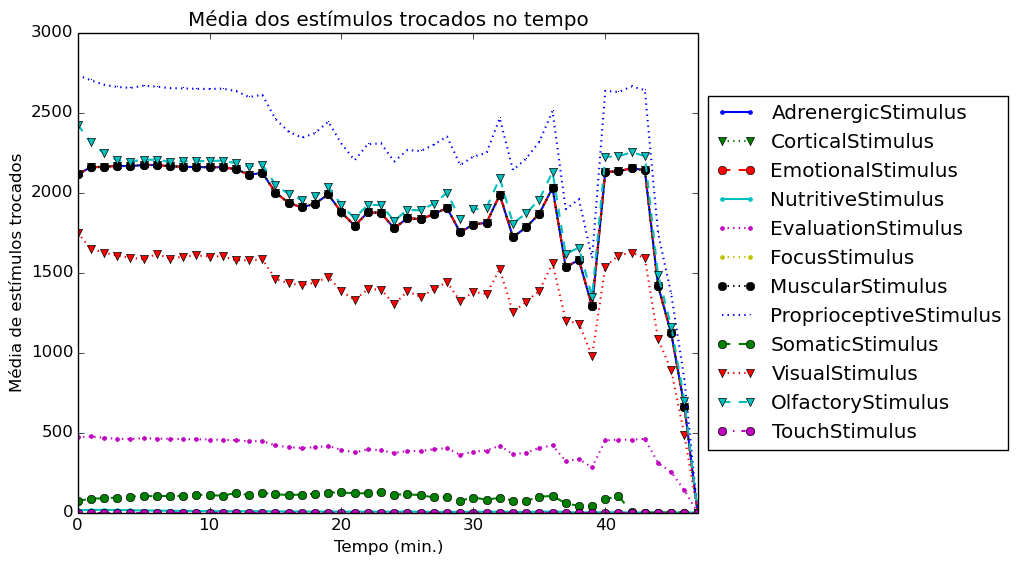
\includegraphics[scale=0.6]{04-figuras/experiments/exp_3/2/avgExchangedStimuliOverTime.png}
  \label{fig:exp_3_2_exchgStimuli}
\end{figure}

\begin{figure}[H]
  \centering
  \caption{Média temporal dos estímulos trocados em simulação utilizando 3 \textit{holders}}
  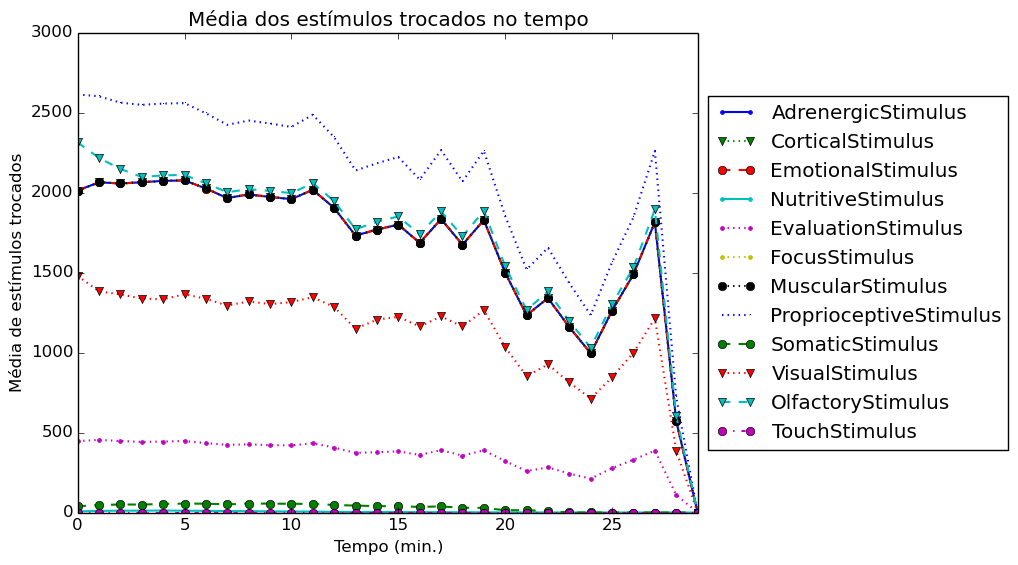
\includegraphics[scale=0.6]{04-figuras/experiments/exp_3/3/avgExchangedStimuliOverTime.png}
  \label{fig:exp_3_3_exchgStimuli}
\end{figure}

\begin{figure}[H]
  \centering
  \caption{Média temporal dos estímulos trocados em simulação utilizando 4 \textit{holders}}
  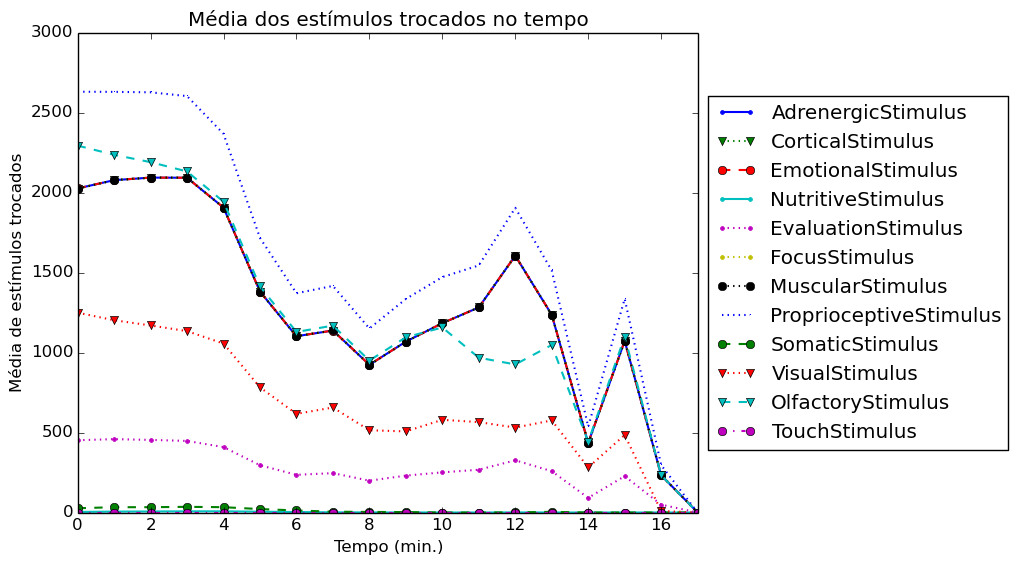
\includegraphics[scale=0.6]{04-figuras/experiments/exp_3/4/avgExchangedStimuliOverTime.png}
  \label{fig:exp_3_4_exchgStimuli}
\end{figure}

\begin{figure}[H]
  \centering
  \caption{Média temporal dos estímulos trocados em simulação utilizando 5 \textit{holders}}
  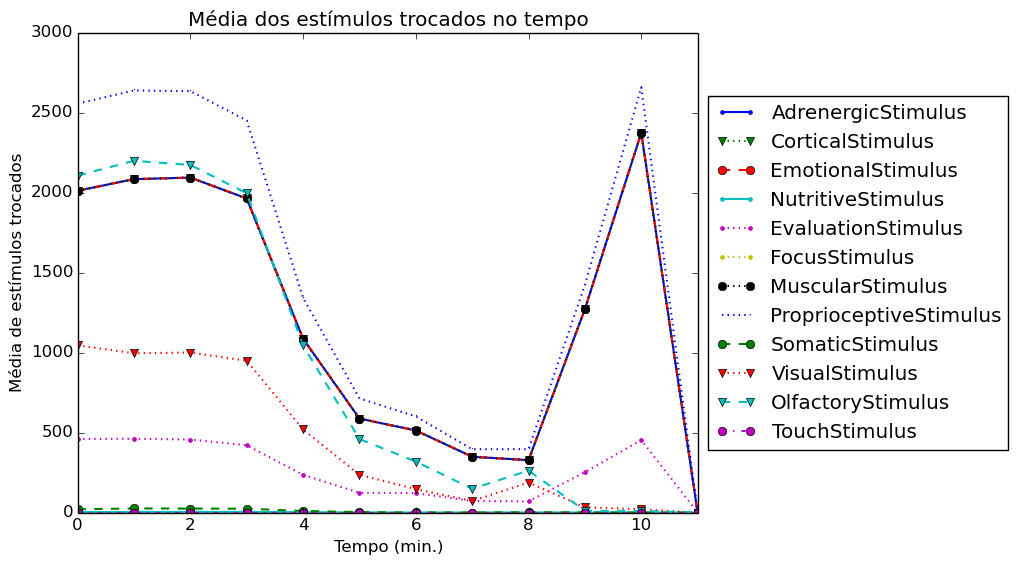
\includegraphics[scale=0.6]{04-figuras/experiments/exp_3/5/avgExchangedStimuliOverTime.png}
  \label{fig:exp_3_5_exchgStimuli}
\end{figure}

A medida que o tempo evolui e as criaturas morrem o erro relativo aumenta, e os dados próximos ao final do eixo temporal não tem confiabilidade estatística. Os gráficos da evolução do erro relativo no tempo estão apresentados na \autoref{ap:erroExp3}.

\section{Síntese dos resultados}
\label{sec:sintese}

%% exp 1
A respeito do primeiro experimento, não é possível fazer uma comparação quantitativa entre as duas arquiteturas pois ambas foram configuradas com o $\Delta_{sym}$ diferentes. Esse parâmetro exerce forte influência na dinâmica interna das criaturas e uma alteração da ordem de centésimos pode aumentar o tempo de vida em dias.  Assim, ele foi calibrado de modo que o tempo de execução das simulações fosse de no máximo uma hora, tempo que pareceu aceitável para observar o comportamento do sistema.  Entretanto o Artífice e DL2L são qualitativamente semelhantes, principalmente no que diz respeito a dinâmica interna das criaturas. Por exemplo, na \autoref{fig:accNutrients} é possível notar uma tendência semelhante na escolha de nutrientes. Ambas as arquiteturas começam escolhendo nutrientes a uma tendência parecida, quando o Artífice, por volta dos 10 minutos (\autoref{fig:accNutrients_artifice}) tem uma redução na escolha de nutrientes do tipo GRA. Este evento acontece por volta do mesmo instante de tempo na arquitetura DL2L.

É possível observar uma variação brusca na troca de estímulos proprioceptivos da arquitetura Artífice (\autoref{fig:exchgStimuli_artifice}), o que não acontece de forma tão brusca no segundo gráfico. Junto a isso, a DL2L parece exibir um comportamento mais estável ao longo do tempo comparada a sua antecessora. Uma hipótese para esses fenômenos pode estar na alocação dos componentes nas duas arquiteturas, que acontece de modo diferente. No Artífice uma \textit{thread} é escalonada para tratar estímulos, caso ela não encontre nenhum no \textit{pool} compartilhado ela entra em estado de espera até ser notificiada novamente, trata os estímulos, e entra em estado de espera por um tempo $T$ que varia de componente para componente. Essa \textit{thread} pode ser acordada após o período de espera ou durante ele (o que é chamado de \textit{spurious wakeup}), fazendo com que a execução de um componente possa vir de vários fluxos diferentes, e não necessariamente haverá estímulo para ser tratado. Por outro lado, o \textit{toolkit} Akka garante que um ator só é escalonado na presença de mensagens.

No uso dos mecanismos de escolha há uma discrepância entre as arquiteturas, enquanto na \autoref{fig:accChoices_artifice} as escolhas aleatórias praticamente acompanham as escolhas por \textit{affordances}, na \autoref{fig:accChoices_dl2l} as escolhas aleatórias estabilizam muito abaixo do outro mecanismo. Para explicar esse comportamento pode-se levantar uma hipótese sobre a velocidade e quantidade de estímulos que são recebidos e tratados pelos componentes simultaneamente. No Artífice, os componentes do sistema nervoso são escalonados para tratar estímulos à uma taxa fixa, o que leva a uma acumulação de estímulos no \textit{buffer} compartilhado por eles. Já a arquitetura DL2L tem um caráter reativo, \textit{i.e.}, os componentes reagem somente na presença de estímulo, que não tem uma frequência fixa, com exceção dos estímulos enviados pelo \textit{PartialAppraisal}. Portanto, tão logo um componente recebe um estímulo, ele é escalonado para tratá-lo. Isso diminui o número de estímulos simultâneos, o que reduz o número de \textit{affordances} que a criatura precisa escolher possibilitando uma desambiguação mais efetiva, diminuindo o número de escolhas aleatórias. 

Há uma diferença na eficiência comportamental apresentada na \autoref{fig:behEfficiency} entre as duas arquiteturas. Na \autoref{fig:behEfficiency_artifice} as curvas de tarefa simples e complexas exibem um comportamento mais semelhante ao esperado pelo cálculo da equação descrita na \autoref{eq:behEfficiency}. A \autoref{fig:behEfficiency_dl2l} exibe um comportamento médio aparentemente linear entre os minutos 0 e 31, que precisa ser melhor investigado. Mas a hipótese inicial é de que esse efeito seja somente prolongamento do eixo do tempo.

% exp 2
A partir dos resultados do segundo experimento (\autoref{tab:resumo_exp2}) pode-se observar uma diminuição do tempo de vida, da distância percorrida, e do número de presas comidas. Pelos gráficos da média de estímulos trocados no tempo (Figuras \ref{fig:exchgStimuli_dl2l}, \ref{fig:exp_2_2_exchgStimuli}, \ref{fig:exp_2_3_exchgStimuli}, \ref{fig:exp_2_4_exchgStimuli} e \ref{fig:exp_2_5_exchgStimuli}) é possível observar também uma diminuição de praticamente todos os tipos de estímulos. Posto que a densidade do mundo permanece constante, há reposição de nutrientes durante a simulação, as criaturas não interagem entre sí e por isso são independentes, e a configuração das máquinas é a mesma para todas as simulações, a única mudança entre as configurações é a quantidade de atores que executam sobre a mesma máquina. 

Partindo destes fatos e de que o componente \textit{PartialAppraisal} do SNC é o único componente que funciona à uma taxa fixa e é responsável por manter o metabolismo da criatura em funcionamento, é possível formular a seguinte hipótese sobre a diminuição do tempo de vida e o arrefecimento da troca de estímulos: os componentes são escalonados com uma menor frequência, tratando um número menor de estímulos, não havendo tempo hábil para que o sistema nervoso equilibre a dinâmica interna, levando as criaturas ao óbito mais rapidamente. Um segundo fator que provavelmente influencia na diminuição do tempo de vida médio da simulação é a sobrecarga do detector de colisões, que tem que tratar e enviar um número maior de mensagens, o que aumenta a latência entre a criatura atualizar sua posição no colisor e receber suas novas colisões.

% exp 3
No terceiro experimento é possível observar um fenômeno semelhante ao do segundo: as médias de tempo de vida, nutrientes comidos e distância percorrida diminuem a medida que aumenta o número de \textit{holders} (\autoref{tab:resumo_exp3}). Especialmente nas últimas configurações o tempo de vida diminui drasticamente comparado ao experimento anterior. Ao olhar para a troca de estímulos ao longo do tempo (Figuras \ref{fig:exchgStimuli_dl2l}, \ref{fig:exp_3_2_exchgStimuli}, \ref{fig:exp_3_3_exchgStimuli}, \ref{fig:exp_3_4_exchgStimuli} e \ref{fig:exp_3_5_exchgStimuli}) não há evidência qualitativa de que a maioria deles está diminuindo, salvo os estímulos visuais. Como as criaturas não competem por recursos na mesma máquina, só há o gargalo do detector de colisões, o que explica a diminuição desses estímulos. Como o ritmo da dinâmica continua o mesmo, somente a percepção do mundo fica mais lenta, é natural que as criaturas morram mais rapidamente.

Como dito antes, os resultados descritos acima foram preliminares e permitem apenas levantar algumas hipóteses sobre o funcionamento da DL2L. Para validar as hipóteses levantadas é necessário propor um novo conjunto de experimentos. Adiante, segue a conclusão deste trabalho, que retomará os objetivos iniciais, as principais contribuições e apontará trabalhos futuros.

			% Resultados
% -----------------------------------------------------------------------------
%   Arquivo: ./02-elementos-textuais/conclusao.tex
% -----------------------------------------------------------------------------



\chapter{Conclusão}
\label{chap:conclusao}

A proposta deste trabalho foi propor o modelo e a implementação de um simulador de vida artificial distribuído e assíncrono utilizando o modelo de atores como ferramenta construtitva. Como foi discutido na \autoref{chap:introducao}, há relevância em prover uma arquitetura deste perfil visto que é interessante estudar a modelagem de sistemas biológico em larga escala,  e as técnicas usadas frequentemente na literatura, como concorrência por \textit{threads}, são impeditivas para essa linha de pesquisa.

Como \autoref{chap:fundamentacaoTeorica}, o modelo de programação concorrente baseado em \textit{threads} e memória compartilhada, padece de problemas de sincronização, como condições de corrida, \mbox{\textit{deadlocks}} e \textit{livelocks}, mas é possível evitá-los com o uso correto de \textit{locks}, assumindo que há perda de performance. O modelo de atores abre mão da possibilidade de compartilhamento de memória e adota uma operação estritamente assíncrona, baseado em troca de mensagens. Essa decisão construtiva evita esses problemas de sincronização.A implementação do modelo de atores mais desenvolvida atualmente é o \textit{Akka}, e por isso foi adotada neste trabalho. 

Na área de simulação de processos biológicos, principalmente do processo cognitivo, não existem muitos projetos que pensem a modelagem em termos de sistemas distribuídos e assíncronos. No \autoref{chap:trabRelac} foram apresentados trabalhos que modelam o processo cognitivo, partindo de uma perspectiva dita biológica, mas que no fundo partem de abordagens clássicas simbolistas/conexionistas. A exceção dentre estes trabalhos é o projeto Artífice, uma arquitetura para construção de criaturas artificiais dotadas de sistema nervoso, parte da perspectiva da cognição biológica. Além do mais, este foi construído para ser um sistema multi-agentes não determinístico e assíncrono, característica não  encontrada nos outros trabalhos. Contudo o projeto padecia de problemas de escalabilidade, por ter sido construído utilizando programação concorrente baseada no compartilhamento de estado.

Tendo uma arquitetura cognitiva funcional, fundamentada num arcabouço teórico amplo da modelagem do processo cognitivo, foi proposta uma nova implementação no \autoref{chap:metodologia} baseada no modelo de atores, que permitisse a simulação em ambiente distribuído. A arquitetura proposta, nomeada DL2L tem as mesmas funcionalidades básicas da arquitetura Artífice, no que diz respeito ao processo cognitivo-emocional. Um esquema de persistência foi proposto para que seja possível armazenar e recuperar posteriormente os dados da dinâmica interna e externa das criaturas. Também foi proposto um esquema de distribuição das entidades da simulação de forma que eles sejam logicamente localizáveis em um \textit{cluster}. O modelo possui um único gargalo e ponto único de falha que é a verificação de colisões, que até aqui, é feita de forma centralizada.

O capítulo \autoref{chap:resultados} expõe os resultados dos experimentos preliminares. Estes serviram para avaliar a conformidade qualitativa da arquitetura proposta com a Artífice, tal como a escalabilidade vertical e horizontal do sistema. Os resultados mostraram que, a princípio ambas as arquiteturas são qualitativamente comparáveis. Contudo o projeto DL2L ainda carece de refinamentos, isso pois a tarefa de detecção de colisões parece ficar sobrecarregada quando o número de criaturas aumenta numa taxa pequena. 

\section{Principais contribuições}


Este trabalho deixa como principal contribuição uma arquitetura cognitiva multi-agente para simulação de criaturas artificiais, que opera como um sistema assíncrono distribuído. A arquitetura DL2L é qualitativamente comparável com a arquitetura Artífice, guardadas as diferenças entre os parâmetros intrínsecos e extrínsecos a criatura artificial. Do ponto de vista da engenharia de software, a primeira tem um código muito mais simples, com menos parâmetros para serem calibrados do que a segunda. Isso por que no Artífice havia uma \textit{thread} para cada componente, e era necessário calibrar parâmetros para o ambiente de execução de todas essas \textit{threads}. Na arquitetura DL2L o ambiente de execução está encapsulado pelo \textit{toolkit} Akka. 

Apesar da arquitetura ainda não tornar possível o estudo de simulações de forrageamento em larga escala por sofrer de um problema de único ponto de gargalo/falha, espera-se que resolvido este problema seja possível escalar o sistema em um \textit{cluster}. 


\section{Trabalhos futuros}

Como trabalhos futuros propõe-se estudar outras maneiras de verificar a colisão em um ambiente distribuído de modo a evitar o aumento  da latência a medida que o sistema cresce. Possibilidades que podem ser exploradas a resolver esse problema: checar colisões de mais entidades ao mesmo tempo e responder todas de uma vez, evitando o aumento da quantidade de mensagens enviadas; permitir ao ator que verifica as colisões de criar outros atores que possam assumir a tarefa, aproveitando o paralelismo da máquina; alterar o esquema de alocação das entidades entre os \textit{holders}, de modo que seja possível, dada a posição da criatura, descobrir em tempo constante quais \textit{holders} tem entidades próxima a essa região. É necessário também aprimorar os mecanismos de aprendizagem, adicionando memórias de curto, médio e longo prazo e comparar os resultados com os já vistos na literatura. 


%\section{Considerações Finais}
%\label{sec:consideracoesFinais}

%As derradeiras palavras para encerramento do seu trabalho acadêmico.



% -----------------------------------------------------------------------------
%   OBS: a norma ABNT estabelece que em qualquer tipo de trabalho acadêmico monográfico
%   deve haver um capítulo de conclusão
% -----------------------------------------------------------------------------
				% Conclusão

%   Insere os elementos pós-textuais
\postextual
% -----------------------------------------------------------------------------
%   Arquivo: ./03-elementos-pos-textuais/referencias.tex
% -----------------------------------------------------------------------------



% -----------------------------------------------------------------------------
%   Carrega o arquivo “myRefs.bib” e extrai automaticamente as referências citadas
% -----------------------------------------------------------------------------

\bibliography{./03-elementos-pos-textuais/myRefs}{}
\bibliographystyle{abntex2-alf}		% Define o estilo ABNT para formatar a lista de referências  


% -----------------------------------------------------------------------------
%   Este arquivo não necessita de ser editado.
% -----------------------------------------------------------------------------
		% Referências
%\include{./03-elementos-pos-textuais/glossario}		% Glossário
% -----------------------------------------------------------------------------
%   Arquivo: ./03-elementos-pos-textuais/apendices.tex
% -----------------------------------------------------------------------------



\begin{apendicesenv}
\partapendices
\chapter{Gráficos de erro relativo}

\section{Experimento 1}
\label{ap:erroExp1}

\begin{figure}[H]
    \centering
    \caption{Erro relativo da média de estímulos trocados no tempo para arquitetura Artífice}
    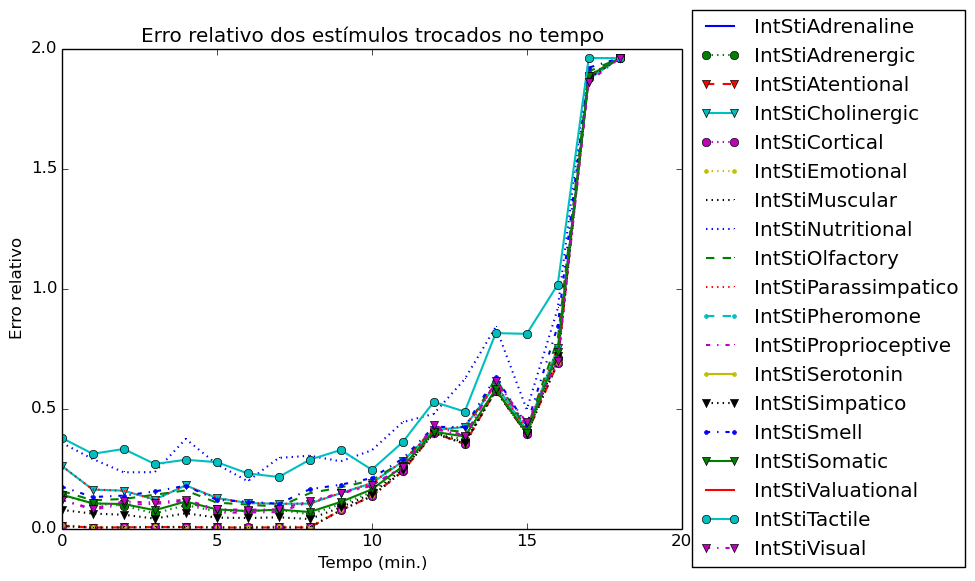
\includegraphics[scale=0.6]{04-figuras/experiments/exp_1_artifice/avgExchangedStimuliOverTime_err.png}
    \label{fig:exchStimuli_artifice_err}
\end{figure}

\begin{figure}[H]
    \centering
    \caption{Erro relativo da média de estímulos trocados no tempo para a arquitetura DL2L}
    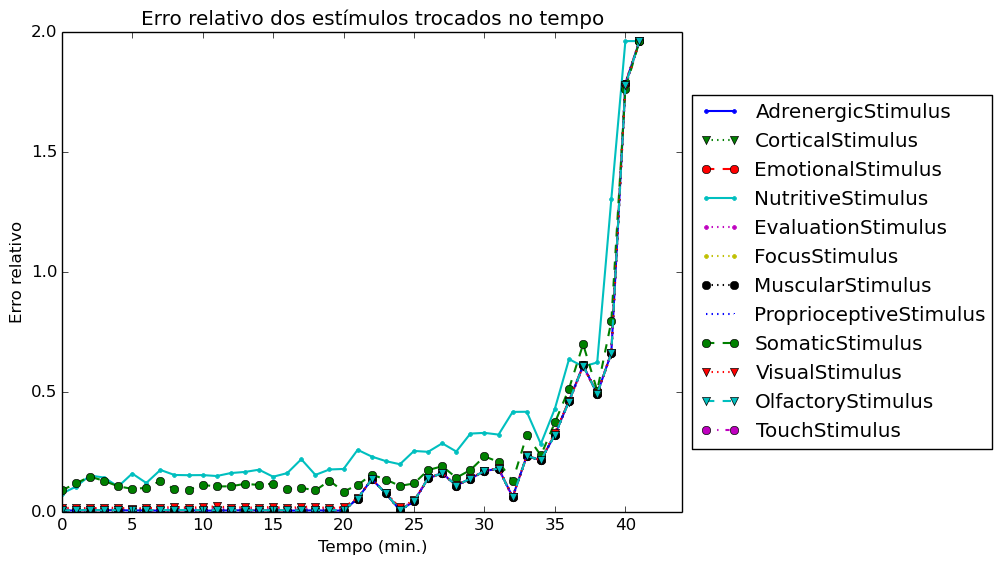
\includegraphics[scale=0.6]{04-figuras/experiments/exp_1_l2l/avgExchangedStimuliOverTime_err.png}
    \label{fig:exchStimuli_dl2l_err}
\end{figure}

\begin{figure}[H]
    \centering
    \caption{Erro relativo da média de escolhas acumuladas no tempo para a arquitetura Artífice}
    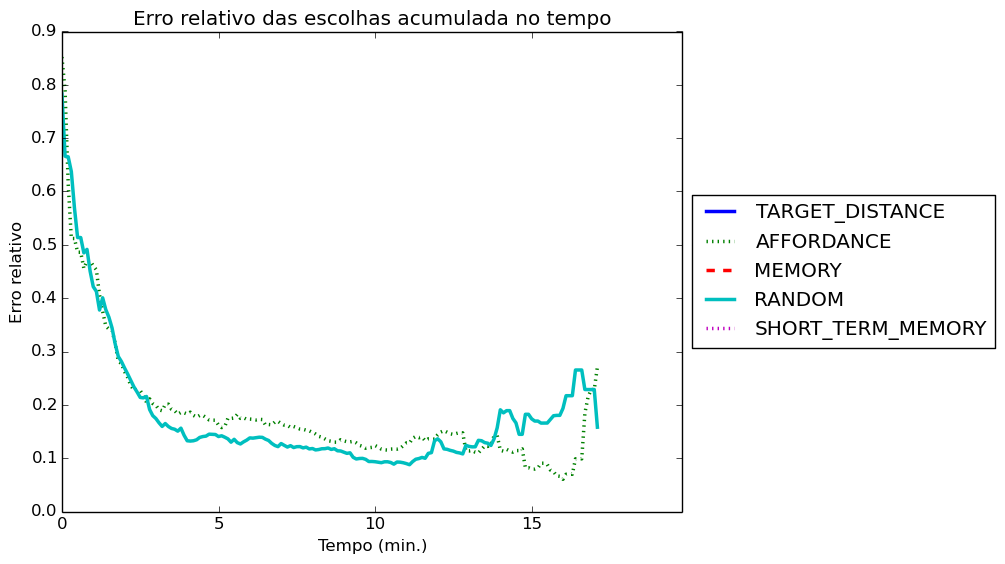
\includegraphics[scale=0.6]{04-figuras/experiments/exp_1_artifice/accumulatedChoices_err.png}
    \label{fig:accChoices_artifice_err}
\end{figure}

\begin{figure}[H]
    \centering
    \caption{Erro relativo da média das escolhas acumuladas no tempo para a arquitetura DL2L}
    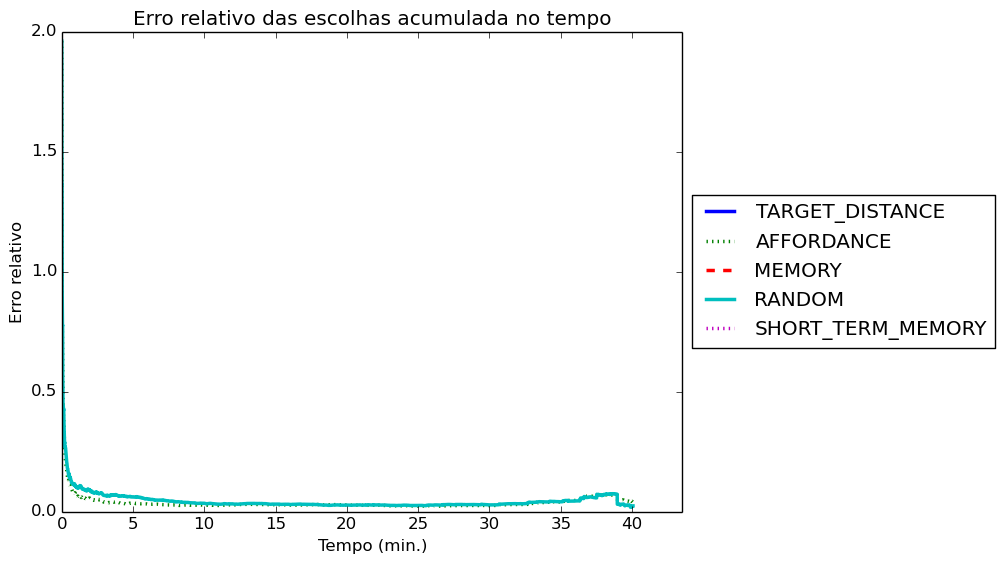
\includegraphics[scale=0.6]{04-figuras/experiments/exp_1_l2l/accumulatedChoices_err.png}
    \label{fig:accChoices_dl2l_err}
\end{figure}

\begin{figure}[H]
    \centering
    \caption{Erro relativo da média da eficiência comportamental no tempo para a arquitetura Artífice}
    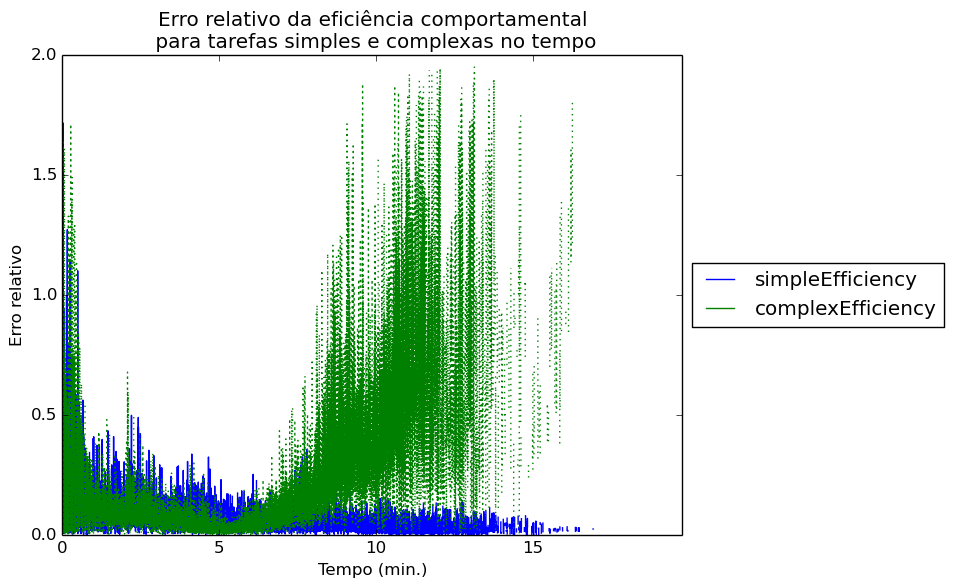
\includegraphics[scale=0.6]{04-figuras/experiments/exp_1_artifice/behaviouralEfficiency_err.png}
    \label{fig:behEfficiency_artifice_err}
\end{figure}

\begin{figure}[H]
    \centering
    \caption{Erro relativo da média da eficiência comportamental no tempo para a arquitetura DL2L}
    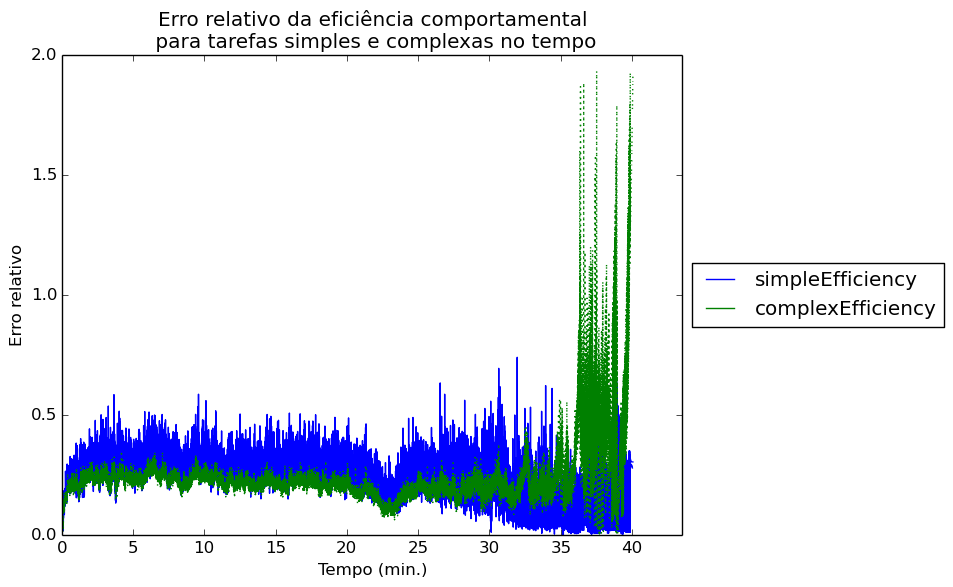
\includegraphics[scale=0.6]{04-figuras/experiments/exp_1_l2l/behaviouralEfficiency_err.png}
    \label{fig:behEfficiency_dl2l_err}
\end{figure}

\begin{figure}[H]
    \centering
    \caption{Erro relativo da média de nutrientes comidos acumulados no tempo para a arquitetura DL2L}
    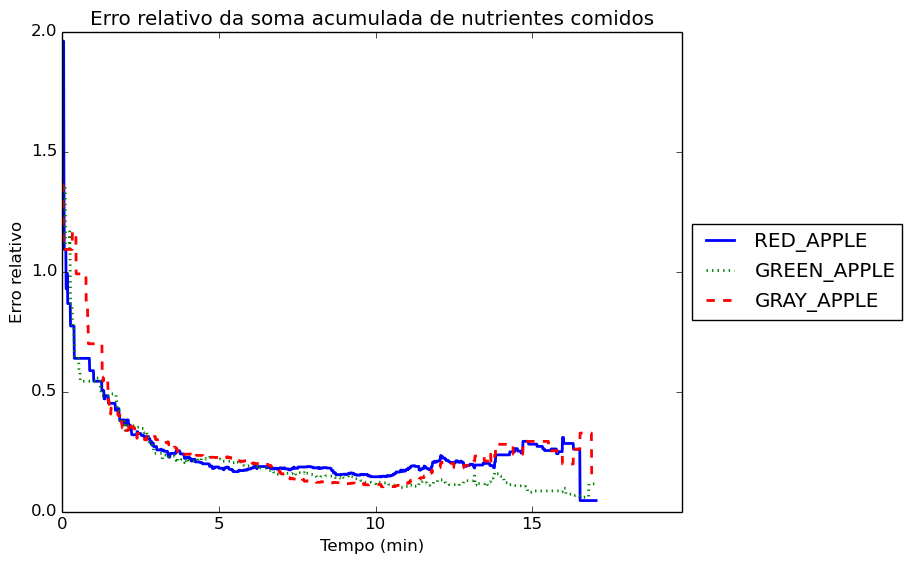
\includegraphics[scale=0.6]{04-figuras/experiments/exp_1_artifice/accumulatedNutrients_err.png}
    \label{fig:accNutrients_artifice_err}
\end{figure}

\begin{figure}[H]
    \centering
    \caption{Erro relativo da média de nutrientes comidos acumulados no tempo para a arquitetura DL2L}
    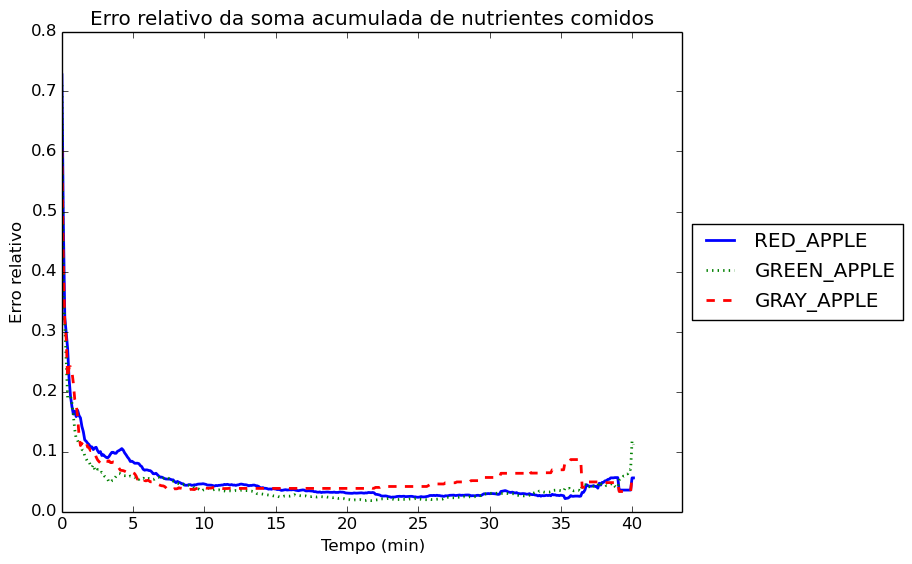
\includegraphics[scale=0.6]{04-figuras/experiments/exp_1_l2l/accumulatedNutrients_err.png}
    \label{fig:accNutrients_dl2l_err}
\end{figure}


\section{Experimento 2}
\label{ap:erroExp2}

\begin{figure}[H]
 \centering
 \caption{Erro relativo da média de estímulos trocados para o experimento 2, com 2 criaturas}
 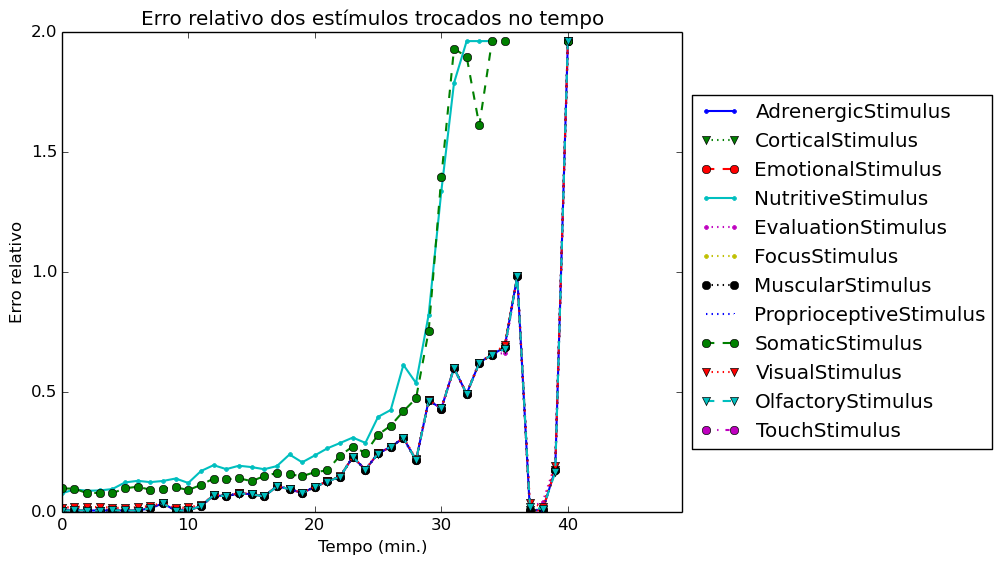
\includegraphics[scale=0.6]{04-figuras/experiments/exp_2/2/avgExchangedStimuliOverTime_err.png}
 \label{fig:exp_2_2_avgExchStimuli_err}
\end{figure}

\begin{figure}[H]
 \centering
 \caption{Erro relativo da média de estímulos trocados para o experimento 2, com 3 criaturas}
 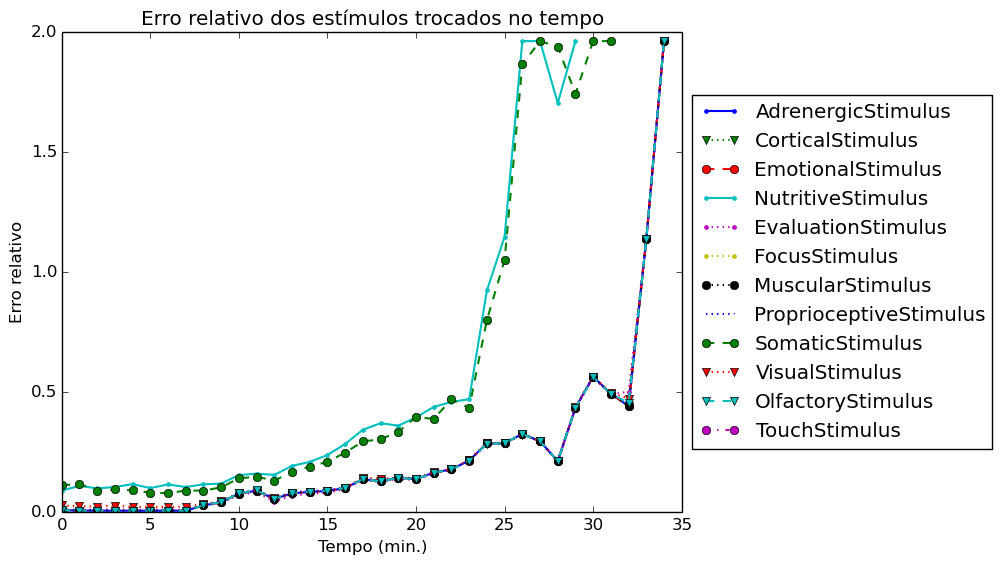
\includegraphics[scale=0.6]{04-figuras/experiments/exp_2/3/avgExchangedStimuliOverTime_err.png}
 \label{fig:exp_2_3_avgExchStimuli_err}
\end{figure}

\begin{figure}[H]
 \centering
 \caption{Erro relativo da média de estímulos trocados para o experimento 2, com 4 criaturas}
 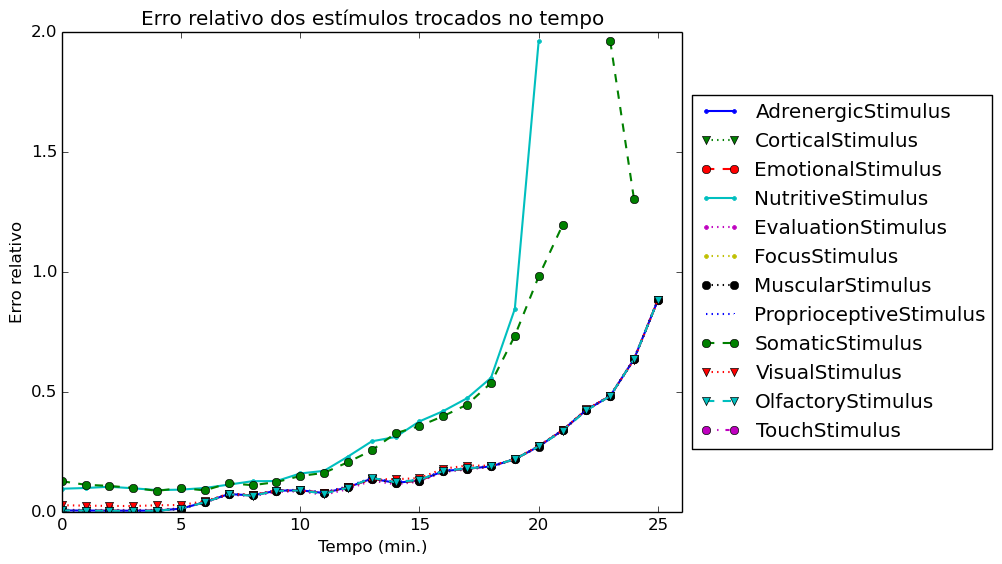
\includegraphics[scale=0.6]{04-figuras/experiments/exp_2/4/avgExchangedStimuliOverTime_err.png}
 \label{fig:exp_2_4_avgExchStimuli_err}
\end{figure}

\begin{figure}[H]
 \centering
 \caption{Erro relativo da média de estímulos trocados para o experimento 2, com 5 criaturas}
 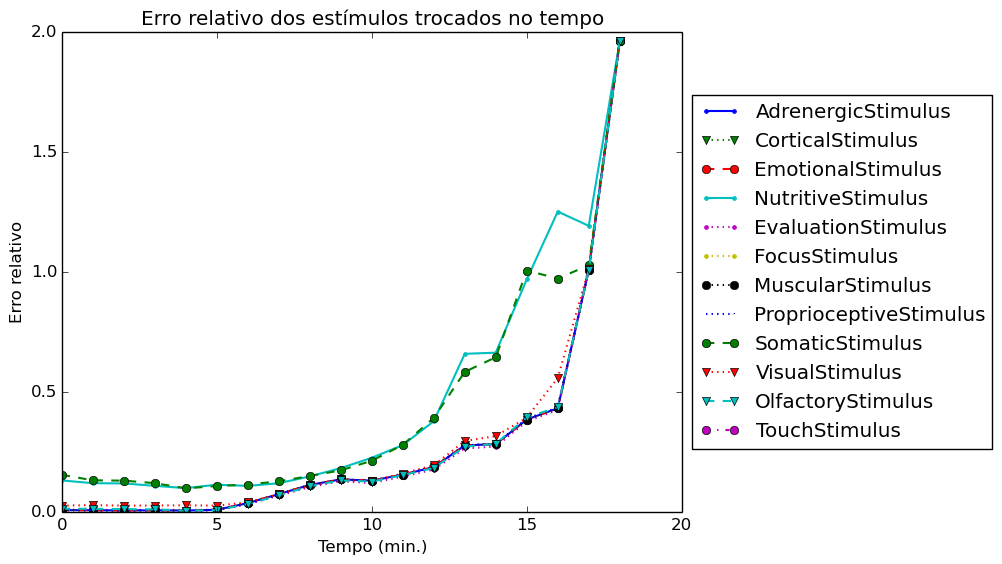
\includegraphics[scale=0.6]{04-figuras/experiments/exp_2/5/avgExchangedStimuliOverTime_err.png}
 \label{fig:exp_2_5_avgExchStimuli_err}
\end{figure}

\section{Experimento 3}
\label{ap:erroExp3}

\begin{figure}[H]
 \centering
 \caption{Erro relativo da média de estímulos trocados para o experimento 3, com 2 \textit{holders}}
 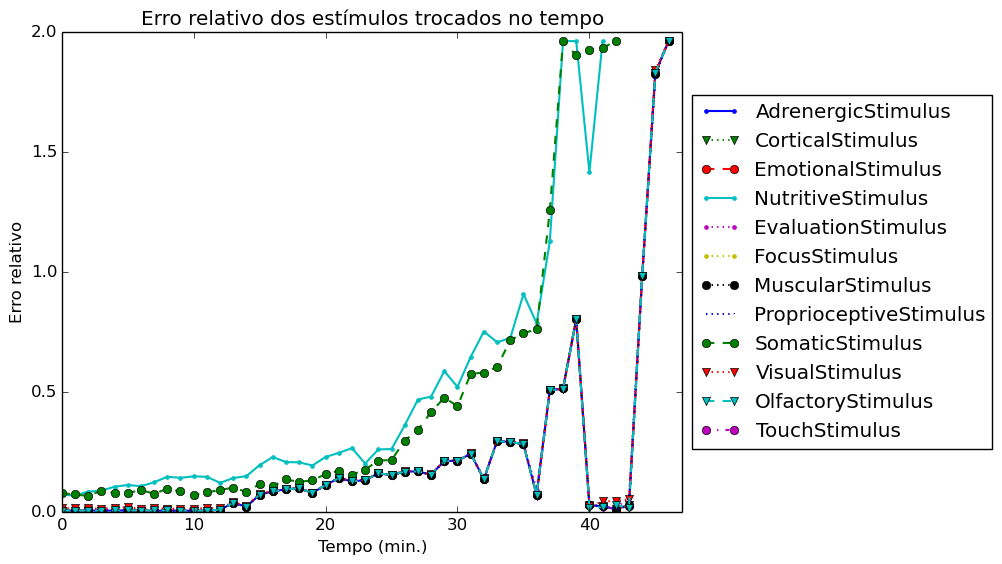
\includegraphics[scale=0.6]{04-figuras/experiments/exp_3/2/avgExchangedStimuliOverTime_err.png}
 \label{fig:exp_3_2_avgExchStimuli_err}
\end{figure}

\begin{figure}[H]
 \centering
 \caption{Erro relativo da média de estímulos trocados para o experimento 2, com 3 \textit{holders}}
 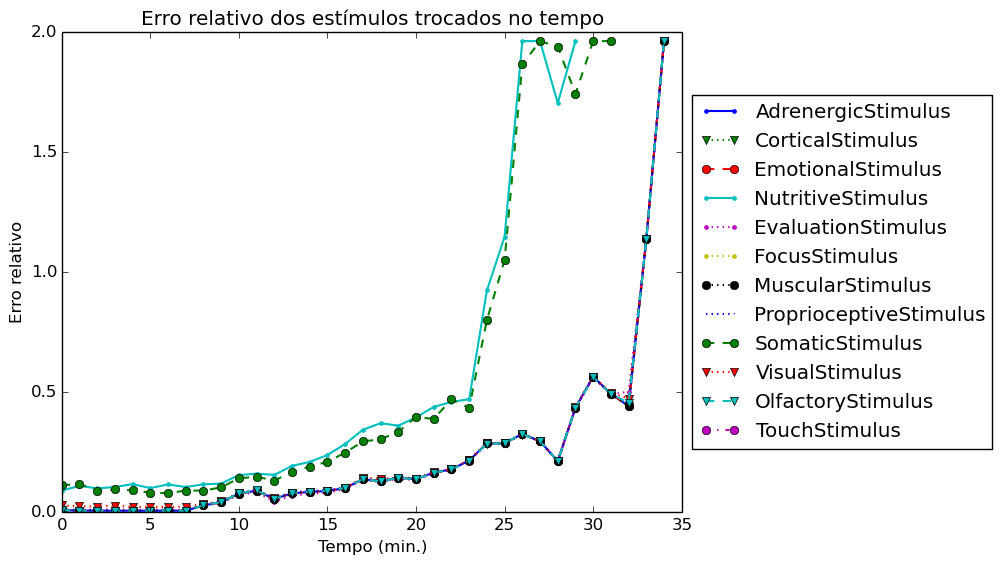
\includegraphics[scale=0.6]{04-figuras/experiments/exp_2/3/avgExchangedStimuliOverTime_err.png}
 \label{fig:exp_3_3_avgExchStimuli_err}
\end{figure}

\begin{figure}[H]
 \centering
 \caption{Erro relativo da média de estímulos trocados para o experimento 2, com 4 \textit{holders}}
 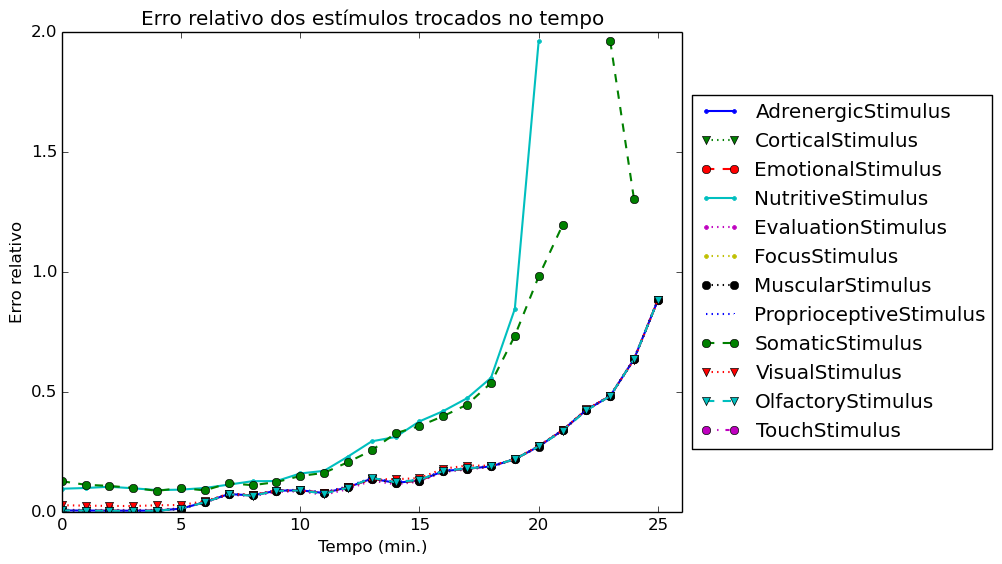
\includegraphics[scale=0.6]{04-figuras/experiments/exp_2/4/avgExchangedStimuliOverTime_err.png}
 \label{fig:exp_3_4_avgExchStimuli_err}
\end{figure}

\begin{figure}[H]
 \centering
 \caption{Erro relativo da média de estímulos trocados para o experimento 2, com 5 \textit{holders}}
 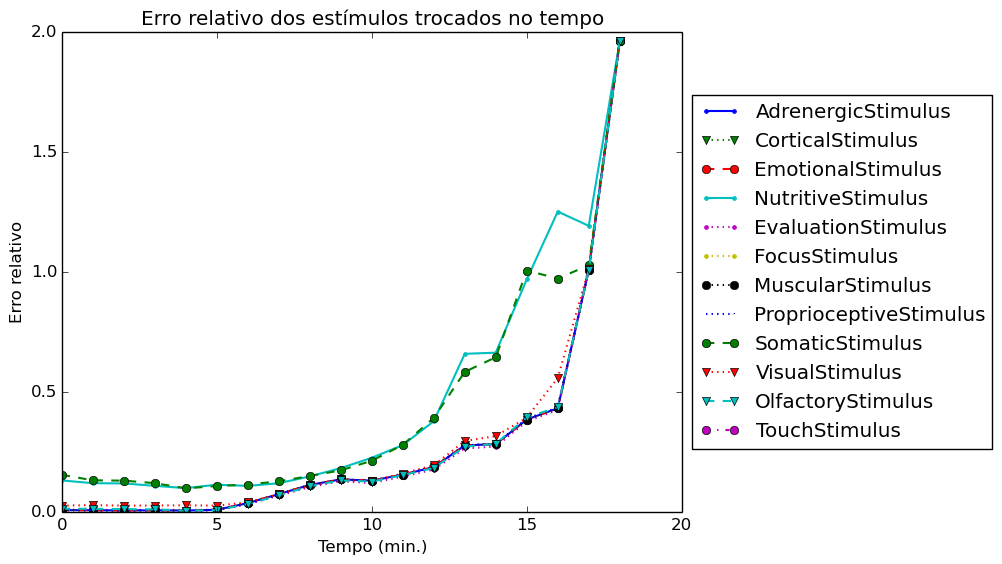
\includegraphics[scale=0.6]{04-figuras/experiments/exp_2/5/avgExchangedStimuliOverTime_err.png}
 \label{fig:exp_3_5_avgExchStimuli_err}
\end{figure}


\begin{comment}
% -----------------------------------------------------------------------------
% Primeiro apêndice
% -----------------------------------------------------------------------------


\chapter{Nome do apêndice} 			% edite para alterar o título deste apêndice
\label{chap:apendiceA}

Lembre-se que a diferença entre apêndice e anexo diz respeito à autoria do texto e/ou material ali colocado.

Caso o material ou texto suplementar ou complementar seja de sua autoria, então ele deverá ser colocado como um apêndice. Porém, caso a autoria seja de terceiros, então o material ou texto deverá ser colocado como anexo.

Caso seja conveniente, podem ser criados outros apêndices para o seu trabalho acadêmico. Basta recortar e colar este trecho neste mesmo documento. Lembre-se de alterar o "label"{} do apêndice.

Não queira colocar tudo que é complementar em um único apêndice. Organize seus apêndices de modo a que, em cada um deles, haja um único tipo de conteúdo. Isso facilita a leitura e compreensão para o leitor do trabalho. É para ele que você escreve.


% -----------------------------------------------------------------------------
% Novo apêndice
% -----------------------------------------------------------------------------

\chapter{Estrutura de trabalhos acadêmicos}
\label{chap:apEstrTrabAcad}


Quanto à estrutura do trabalho acadêmico, esta varia sobremaneira, a depender da conveniência do autor e seu(s) respectivo(s) orientador(es). No entanto, de acordo com as normas ABNT, alguns elementos são obrigatórios.

A título de sugestão, e apenas isso, a \autoref{fig:prjQualif-TeseDT_DissMT} apresenta uma estrutura para um projeto de qualificação de mestrado ou doutorado, conforme a norma \citeonline{NBR14724:2011}.


\begin{figure}[!h]
	\centering
	\caption{Estrutura sugerida de um Projeto de Qualificação para os cursos de Mestrado ou Doutorado}
	\includegraphics[width=0.5\textwidth]{./04-figuras/prjQualif-TeseDT_DissMT}
	%\fonte{\citeonline{CELSO2012}}
	\label{fig:prjQualif-TeseDT_DissMT}
\end{figure}


Já a \autoref{fig:teseDT_DissMT} apresenta uma estrutura para uma tese de doutorado ou dissertação de mestrado, conforme a norma \citeonline{NBR14724:2011}.

Cabe ressaltar que, em todas as figuras, os elementos obrigatórios estão destacados em vermelho, os demais são opcionais.


\begin{figure}[!h]
	\centering
	\caption{Estrutura sugerida de uma Tese de Doutorado ou Dissertação de Mestrado}
	\includegraphics[width=0.5\textwidth]{./04-figuras/teseDT_DissMT}
	%\fonte{\citeonline{CELSO2012}}
	\label{fig:teseDT_DissMT}
\end{figure}


Observe que a estrutura de um projeto de qualificação é muito similar à da tese ou dissertação. A única diferença existente é que num projeto de qualificação o autor certamente terá, via de regra, apenas resultados parciais e preliminares. Além disso, estando o trabalho ainda em andamento, há que se apresentar um cronograma de trabalho que evidencie que o mesmo poderá ser concluído dentro dos prazos estabelecidos pelo programa.


Por fim, como foi dito, este  \emph{template} pode ser utilizado para outros trabalhos acadêmicos. Neste caso, a \autoref{fig:prjPesqAdmissao} apresenta uma sugestão de projeto de pesquisa a ser submetido ao programa para fins de admissão ao mesmo, conforme a norma \citeonline{NBR15287:2005}.

\begin{figure}[!htb]
	\centering
	\caption{Estrutura sugerida de um projeto de pesquisa para admissão ao PPGMMC}
	\includegraphics[width=0.6\textwidth]{./04-figuras/prjPesqAdmissao}
	%\fonte{\citeonline{CELSO2012}}
	\label{fig:prjPesqAdmissao}
\end{figure}

Você deverá editar o arquivo principal {\ttfamily meuTrabalhoAcademico.tex} para fazer os ajustes necessários, reiterando que as estruturas apresentadas são mera sugestão. 

A inclusão de reticências (\ldots) no texto deverá ser feita através de um comando especial denominado \verb|\ldots| \cite{LaTeX2014}. Assim esse comando deverá ser utilizado ao invés da digitação de três pontos.

Para melhor entendimento do uso do estilo de formatação, aconselha-se que o potencial usuário analise os comandos existentes no arquivo {\ttfamily main.tex} e os resultados obtidos no arquivo {\ttfamily main.pdf} depois do processamento pelo software \LaTeX{} + \textsc{Bib}\TeX{} \cite{LaTeX2014,BibTeX2014}.
Recomenda-se a consulta ao material de referência do software para a sua correta utilização \cite{Lamport1986,Buerger1989,Kopka2003,Mittelbach2004}.

Finalmente, este modelo apresenta um arquivo {\ttfamily makefile} para agilizar a compilação do documento \LaTeX{} e do \textsc{Bib}\TeX{}. portanto, para gerar o documento final no formato PDF, basta apenas executar o comando {\ttfamily make all} no linux. Para limpar os arquivos temporários, basta digitar o comando {\ttfamily make clean}.

O estilo de documento utilizado é o {\ttfamily abntex2}.
Através desse estilo a constituição do documento torna-se facilitada, uma vez que o mesmo possui comandos especiais para auxiliar a distribuição/definição das diversas partes constituintes do projeto.
Esse estilo é baseado nas normas da ABNT\index{ABNT}.

Maiores detalhes relacionados aos comandos existentes no estilo poderão ser adquiridos através da documentação disponível no site \href{https://code.google.com/p/abntex2/}{https://code.google.com/p/abntex2/} \cite{abnTeX22014b}.

Uma das principais vantagens do uso do estilo de formatação para \LaTeX{}  é a formatação \textit{automática} dos elementos que compõem um documento acadêmico, tais como capa, folha de rosto, dedicatória, agradecimentos, epígrafe, resumo, abstract, listas de figuras, tabelas, siglas e símbolos, sumário, capítulos, referências, etc.



% -----------------------------------------------------------------------------
% Novo apêndice
% -----------------------------------------------------------------------------

\chapter{Sobre as ilustrações}
\label{chap:apSobreIlust}

A seguir ilustra-se a forma de incluir ilustrações no corpo do texto. Pela norma figuras, tabelas, quadros, equações, quadros, algoritmos, diagrama, etc. são tipos específicos de ilustrações. As ilustrações (pelo menos alguns tipos específicos) serão indexadas automática em suas respectivas listas.

A numeração sequencial de figuras, tabelas e equações ocorre de modo automático.

Referências cruzadas são obtidas através dos comandos \verb|\label{}| e \verb|\ref{}|. Por exemplo, não é necessário saber que o número de certo capítulo é \ref{chap:fundamentacaoTeorica} para colocar o seu número no texto. Alternativamente se pode usar desta forma: \autoref{chap:fundamentacaoTeorica}. Isto facilita muito a inserção, remoção ou relocação de elementos numerados no texto (fato corriqueiro na escrita e correção de um documento acadêmico) sem a necessidade de renumerá-los todos.



\section{Figuras}
\label{sec:figuras}

Abaixo é apresentado um exemplo de figura.

A \autoref{fig:kdtree} aparece automaticamente na lista de figuras.

Para uso avançado de imagens no \LaTeX{}, recomenda-se a consulta de literatura especializada \cite{Goossens2007}.

\begin{figure}[!htb]
	\centering
	\caption{Exemplo da estrutura de uma árvore KD}
	\includegraphics[width=0.5\textwidth]{./04-figuras/figkdtree}
	\fonte{\citeonline{Souza2012}}
	\label{fig:kdtree}
\end{figure}



\section{Quadros e tabelas}
\label{sec:tabelas}

Também é apresentado o exemplo do \autoref{qua:comparabd} e da \autoref{tab:testes}, que aparece automaticamente na lista de quadros e tabelas.

Informações sobre a construção de tabelas no \LaTeX{} podem ser encontradas na literatura especializada \cite{Lamport1986,Buerger1989,Kopka2003,Mittelbach2004}.

\begin{quadro}[!htb]
	\centering
	\caption{Hierarquia de restrições das questões.\label{qua:comparabd}}
	\begin{tabular}{|p{7cm}|p{7cm}|}
		\hline
		\textbf{BD Relacionais} & \textbf{BD Orientados a Objetos} \\
		\hline
		Os dados são passivos, ou seja, certas operações limitadas podem ser automaticamente acionadas quando os dados são usados. Os dados são ativos, ou seja, as solicitações fazem com que os objetos executem seus métodos. & Os processos que usam dados mudam constantemente. \\
		\hline
	\end{tabular}
	\fonte{\citeonline{Carvalho2001}}
\end{quadro}


Muitos confundem, mas existem diferenças entre tabelas e quadros.

Um quadro é formado por linhas horizontais e verticais, sendo, portanto ``fechado''. Você deverá utilizar um quadro quando o conteúdo é majoritariamente não-numérico. O número do quadro e o título vem acima do quadro, e a fonte, deve vir abaixo.

Uma tabela é formada apenas por linhas verticais, sendo, portanto ``aberta''. Você deverá utilizar uma tabela quando o conteúdo é majoritariamente numérico. O número da tabela e o título vem acima da tabela, e a fonte, deve vir abaixo, tal como no quadro.

Exemplo de tabela:

\begin{table}[!htb]
	\centering
	\caption[Resultado dos testes]{Resultado dos testes.
	\label{tab:testes}}
	\begin{tabular}{rrrrr}
		\toprule
			& Valores 1 & Valores 2 & Valores 3 & Valores 4 \\
		\midrule
			Caso 1 & 0,86 & 0,77 & 0,81 & 163 \\
			Caso 2 & 0,19 & 0,74 & 0,25 & 180 \\
			Caso 3 & 1,00 & 1,00 & 1,00 & 170 \\
		\bottomrule
	\end{tabular}
\end{table}




\section{Equações}
\label{sec:equacoes}

A transformada de Laplace é dada na \autoref{eq:laplace}, enquanto a Eq. \ref{eq:dft} apresenta a formulação da transformada discreta de Fourier bidimensional\footnote{Deve-se reparar na formatação esteticamente perfeita destas equações.}. Observe que utilizamos propositalmente duas formas distintas para referenciar as equações.

\begin{equation}
	X(s) = \int\limits_{t = -\infty}^{\infty} x(t) \, \text{e}^{-st} \, dt
	\label{eq:laplace}
\end{equation}

\begin{equation}
	F(u, v) = \sum_{m = 0}^{M - 1} \sum_{n = 0}^{N - 1} f(m, n) \exp \left[ -j 2 \pi \left( \frac{u m}{M} + \frac{v n}{N} \right) \right]
	\label{eq:dft}
\end{equation}



\section{Algoritmos}\label{sec:algoritmos}

Os algoritmos devem ser feitos segundo o modelo abaixo. Para isso, utilizar o pacote {\ttfamily algorithm2e} no início do arquivo principal como neste exemplo.
\\
\\

\begin{algorithm}
	\caption{Algoritmo para remoção aleatória de vértices}
	\KwIn{o número $n$ de vértices a remover, grafo original $G(V, E)$}
	\KwOut{grafo reduzido $G'(V,E)$}
	$removidos \leftarrow 0$ \\
	\While {removidos $<$ n } {
		$v \leftarrow$ Random$(1, ..., k) \in V$ \\
			\For {$u \in adjacentes(v)$} {
				remove aresta (u, v)\\
				$removidos \leftarrow removidos + 1$\\
			}
			\If {há  componentes desconectados} {
				remove os componentes desconectados\\
			}
		}
\end{algorithm}




% -----------------------------------------------------------------------------
% Novo apêndice
% -----------------------------------------------------------------------------

\chapter{Sobre as listas}
\label{chap:apSobreLista}


Para construir listas de "\textit{bullets}"{} ou listas enumeradas, inclusive listas aninhadas, é utilizado o pacote \verb|paralist|.

O exemplo a seguir ilustra duas listas não numeradas aninhadas, utilizando o ambiente \verb|\compactitem|. Observe a indentação, bem como a mudança automática do tipo de "\textit{bullet}"{} nas listas aninhadas.



\begin{compactitem}
	\item item não numerado 1
	\item item não numerado 2
	\begin{compactitem}
		\item subitem não numerado 1
		\item subitem não numerado 2
		\item subitem não numerado 3
	\end{compactitem}
	\item item não numerado 3
\end{compactitem}


Por outro lado, o exemplo a seguir ilustra duas listas numeradas aninhadas, utilizando o ambiente \verb|\compactenum|. Observe a numeração progressiva e indentação das listas aninhadas.


\begin{compactenum}
	\item item numerado 1
	\item item numerado 2
	\begin{compactenum}
		\item subitem numerado 1
		\item subitem numerado 2
		\item subitem numerado 3
	\end{compactenum}
	\item item numerado 3
\end{compactenum}

Cabe ressaltar que os ambientes \verb|\itemize| e \verb|\enumerate| podem ser utilizados alternativamente. No entanto, durante a compilação pdflatex são apresentados erros associados a estes ambientes, porém o pdf é gerado corretamente. Trata-se de um "\textit{bug}"{} que ainda não conseguimos resolver. Caso conheça a solução, por favor, comunique-nos para que possamos incluí-la numa futura atualização deste modelo.




% -----------------------------------------------------------------------------
% Novo apêndice
% -----------------------------------------------------------------------------

\chapter{Sobre citações e chamadas de referências}
\label{chap:apSobreCita}


Citações são trechos transcritos ou informações retiradas das publicações consultadas para a realização do trabalho.
As citações são utilizadas no texto com o propósito de esclarecer, completar, embasar ou corroborar as ideias do autor.

Todas as publicações consultadas e efetivamente utilizadas (por meio de citações) devem ser listadas, obrigatoriamente, nas referências bibliográficas, de forma a preservar os direitos autorais e intelectuais.

A norma ABNT NBR:10520-2002 classifica as citações em: citações livres e citações literais.



\section{Citações livres}
\label{sec:citacoesLivres}


Nas citações livres, reproduzem-se as ideias e informações de um autor, sem, entretanto, ``copiar letra por letra'' o texto do autor. Sendo assim, não há muito a dizer sobre como fazer citações livres, exceto que há que se tomar o devido cuidado com o "recortar e colar e modificar"{} para que não se caracterize plágio.

Quanto à chamada da referência, ela pode ser feita de duas maneiras distintas, conforme o nome do(s) autor(es) façam parte do seu texto ou não. Os exemplos a seguir ilustram estas duas possibilidades.

Enquanto \citeonline{Maturana2003} defendem uma epistemologia baseada na biologia. Para os autores, é necessário rever \ldots.

Por outro lado, \citeonline{Barbosa2004} contra-argumenta afirmando que \ldots.

Acima, as chamadas de referências foram feitas com o comando \verb|\citeonline{chave}|, que produzirá a formatação correta, conforme a norma ABNT.

 Observe que em ambos os casos anteriores, a frase fica incompleta e incompreensível caso as palavras "Maturana e Varela"{} e "Barbosa et al."{} não sejam "pronunciadas"{}. Ou seja, os nomes dos autores fazem parte da frase. Neste caso, a formatação automática da chamada de referência coloca os nomes dos autores seguido, entre parêntesis pelo ano de publicação da obra referenciada. Isso apenas no caso em que se usa o esquema autor-ano, que é \textit{padrão} neste modelo \LaTeX{}.

A segunda maneira de fazer uma chamada de referência deve ser utilizada quando se quer evitar uma interrupção na sequência do texto, o que poderia, eventualmente, prejudicar a leitura.

Assim, a citação livre é feita e imediatamente após a obra referenciada deve ser colocada entre parênteses. Porém, neste caso específico, o nome do autor deve vir em caixa alta, seguido do ano da publicação, como nos exemplos a seguir.

Há defensores da epistemologia baseada na biologia que argumentam em favor da necessidade de \ldots \cite{Maturana2003}.

Por outro lado, há os que contra-argumentam afirmando que \ldots  \cite{Barbosa2004}.

Nos dois casos imediatamente acima a chamada de referência deve ser feita com o comando \verb|\cite{chave}|, que produzirá a formatação correta, conforme a norma ABNT.

Observe que o estilo de redação das frases teve que ser modificado para torná-las compreensíveis sem a menção explícita dos nomes dos autores. Estes agora não são parte integrante da frase, ficam entre parêntesis. Neste caso, a formatação automática da chamada de referência coloca, entre parêntesis, os nomes dos autores seguido pelo ano de publicação da obra referenciada. Novamente, apenas no caso em que se usa o esquema autor-ano, que é \textit{padrão} neste modelo \LaTeX{}.

Por fim, cabe chamar a atenção para o detalhe do termo \textit{et al.} que deve ser utilizado quando o trabalho citado possui mais de três autores. Esse recurso é automatizado pelo estilo {\ttfamily abntex2}. Caso não haja desejo em abreviar o nome dos demais autores através do termo \textit{et al.}, deve-se incluir a opção {\ttfamily abnt-no-etal-label}. 



\section{Citações literais}
\label{sec:citacoesLiterais}

Nas citações literais, reproduzem-se as ideias e informações de um autor, exatamente como este a expressou, ou seja, faz-se uma ``cópia letra por letra'' do texto do autor. Sendo assim, obviamente, a obra citada deve ser referenciada, sob pena de se caracterizar plágio.

Quanto à chamada da referência, ela pode ser feita de qualquer das duas maneiras mencionadas na \autoref{sec:citacoesLivres}, conforme o nome do(s) autor(es) façam parte do seu texto ou não.

Há duas maneiras distintas de se fazer uma citação literal, conforme o trecho citado seja longo ou curto.

Quando o trecho citado é longo (4 ou mais linhas) deve-se usar um parágrafo específico para a citação, na forma de um texto recuado (4 cm da margem esquerda), com tamanho de letra menor do aquela utilizada no texto e espaçamento entrelinhas simples. Veja o exemplo abaixo.

\begin{citacao}
	Desse modo, opera-se uma ruptura decisiva entre a reflexividade filosófica, isto é a possibilidade do sujeito de pensar e de refletir, e a objetividade científica. 	Encontramo-nos num ponto em que o conhecimento científico está sem consciência. Sem consciência moral, sem consciência reflexiva e também subjetiva. Cada vez mais o desenvolvimento extraordinário do conhecimento científico vai tornar menos praticável a própria possibilidade de reflexão do sujeito sobre a sua pesquisa \cite[p.~28]{Silva2000}.
\end{citacao}

Para se criar o efeito demonstrado na citação anterior, deve-se utilizar o comando:

\begin{verbatim}
\begin{citacao}
<citacao>
\end{citacao}
\end{verbatim}

Acima, para a chamada da referência o comando \verb|\cite[p.~28]{Silva2000}| foi utilizado, visto que os nomes dos autores não são parte do trecho citado.

Observe ainda que foi indicado o número da página da obra citada que contém o trecho citado. A localização precisa do trecho citado deve ser indicada sempre, exceto para artigos científicos (tipicamente com poucas páginas, o que geralmente não é o caso de artigos de revisão de literatura) e outros documentos com "poucas"{} páginas.

Alternativamente, é possível construir uma frase que contenha os autores, e irá encaminhar (por assim dizer) a citação literal. Assim sendo, note que pode após a citação literal não mais aparece o nome dos autores, visto que já se encontra no texto. Veja o exemplo seguinte.

No entanto, \citeonline[p.~33]{Silva2000}, ao fazerem as suas críticas à ciência moderna, afirmam:

\begin{citacao}
	Mas o curioso é que o conhecimento científico que descobriu os meios realmente extraordinários para, por exemplo, ver aquilo que se passa no nosso sol, para tentar conceber a estrutura das estrelas extremamente distantes, e até mesmo para tentar pesar o universo, o que é algo de extrema utilidade, o conhecimento científico que multiplicou seus meios de observação e de concepção do universo, dos objetos, está completamente cego, se quiser considerar-se apenas a si próprio!
\end{citacao}


Já quando o trecho citado é curto (3 ou menos linhas) ele deve inserido diretamente no texto entre aspas. Veja os dois exemplos seguintes, cada qual utilizando uma forma de chamada de referência.

A epistemologia baseada na biologia parte do princípio de que ``assumo que não posso fazer referência a entidades independentes de mim para construir meu explicar'' \cite[p.~35]{Maturana2003}.

A epistemologia baseada na biologia de \citeonline[p.~35]{Maturana2003} parte do princípio de que ``assumo que não posso fazer referência a entidades independentes de mim para construir meu explicar''.

Finalmente, e isto vale para citações curtas ou longas, caso seja necessário inserir ou suprimir (modificar de modo geral) qualquer palavra ou frase no trecho citado literalmente, qualquer que seja a finalidade, isto deve ser feito colocando sua intervenção entre colchetes retos e deve ser indicado explicitamente ao final da citação. Veja o exemplo seguinte.

A epistemologia baseada na biologia parte do princípio de que ``assumo que não posso fazer referencia [\textit{sic}] a \underline{entidades independentes} de mim [realidade objetiva] para construir meu explicar'' \cite[p.~35, comentários e grifo nosso]{Maturana2003}.



\section{Mais detalhes sobre as chamadas de referências}
\label{sec:referUtilizadas}


A seguir há mais exemplos dos comandos para as chamadas de referências e o resultado produzido.


\citeonline{Maturana2003} \ \ \  \verb|\citeonline{Maturana2003}|\\
\citeonline{Barbosa2004} \ \ \   \verb|\citeonline{Barbosa2004}|\\
\cite[p.~28]{Silva2000} \ \ \  \verb|\cite[p.~28]{Silva2000}|\\
\citeonline[p.~33]{Silva2000} \ \ \   \verb|\citeonline[p.~33]{v}|\\
\cite[p.~35]{Maturana2003} \ \ \   \verb|\cite[p.~35]{Maturana2003}|\\
\citeonline[p.~35]{Maturana2003} \ \ \   \verb|\citeonline[p.~35]{Maturana2003}|\\
\cite{Barbosa2004,Maturana2003} \ \ \   \verb|\cite{Barbosa2004,Maturana2003}|\\


Há que se tomar bastante cuidado com referências cujos autores têm nomes compostos, tipo João de Souza Júnior ou Antônio José da Silva Filho. Para que a formatação seja correta, os nomes dos autores no arquivo {\ttfamily .bib} deverá ser cadastrado de uma forma específica. Para maiores detalhes, veja o \autopageref{chap:anexoB} \footnote{O texto do anexo é de inteira responsabilidade do autor devidamente referenciado.}.

Os exemplos abaixo ilustram a formatação correta.


\cite[p.~28]{vanGELDER1998} \ \ \ \ \  \verb|\cite[p.~28]{vanGELDER1998}|\\
\citeonline[p.~28]{vanGELDER1998} \ \ \ \ \  \verb|\citeonline[p.~28]{vanGELDER1998}|\\
\cite[p.~35]{Silva2013} \ \ \ \ \  \verb|\cite[p.~35]{Silva2013}|\\
\citeonline[p.~35]{Silva2013} \ \ \ \ \  \verb|\citeonline[p.~35]{Silva2013}|\\


Observe que, a despeito do que está dito no \autoref{chap:anexoB}, ainda há falhas na formatação ABNT de nomes tipo \verb|van Gelder| quando utilizados em chamadas de referências que fazem parte do texto (\textit{e.g.}, \verb|\citeonline{vanGELDER1998}| que deveria produzir \verb|van Gelder (1998)|). Este problema pode ser contornado facilmente, simplesmente evitando o uso dessa forma de chamada de referência, preferindo sempre nestes casos, o uso da forma \textit{e.g.}, \verb|\cite{vanGELDER1998}| que será formatada corretamente, produzindo \verb|(van GELDER, 1998)|.

Observe ainda o caso em que é feita duas citações juntas \cite{Santos2003, Neubert2001, Silva2013} e como citar endereços Web \cite{IRL2014}. 




% -----------------------------------------------------------------------------
% Novo apêndice
% -----------------------------------------------------------------------------

\chapter{Sobre as referências bibliográficas}
\label{chap:apSobreRefer}

A bibliografia é feita no padrão \textsc{Bib}\TeX{}. As referências são colocadas em um arquivo separado. Os elementos de cada item bibliográfico que devem constar nas referências  bibliográficas são apresentados a seguir. Tais referências bibliográficas devem seguir a norma \citeonline{NBR6023:2002} da ABNT\footnote{As normas técnicas da ABNT não são gratuitas.}.



\section{Entradas de referências}
\label{sec:entradasRefs}

Entradas são objetos de citação bibliográficas. Dito de outra forma, são as categorias dos tipos de documentos e materiais componentes da bibliografia. A classe abn\TeX{} define as seguintes entradas:


\begin{verbatim}
@book
@inbook
@article
@phdthesis
@mastersthesis
@monography
@techreport
@manual
@proceedings
@inproceedings
@journalpart
@booklet
@patent
@unpublished
@misc
\end{verbatim}

Cada entrada é formatada pelo pacote \citeonline{abnTeX22014d} de uma forma específica. Algumas entradas foram introduzidas especificamente para atender à norma \citeonline{NBR6023:2002}, são elas: \verb|@monography|, \verb|@journalpart|,\verb|@patent|. As demais entradas são padrão \textsc{Bib}\TeX{}. Para maiores detalhes, refira-se a \citeonline{abnTeX22014d}, \citeonline{abnTeX22014b}, \citeonline{abnTeX22014c}.

A entrada \verb|@monography| é utilizada para cadastrar referências a trabalhos de conclusão de curso, monografias de cursos de especialização (pós-graduação \textit{lato sensu}), e outros trabalhos monográficos, exceto dissertação de mestrado e tese de doutorado. Eu particularmente, não considero que a formatação deste tipo de entrada está adequado. Para um trabalho de conclusão de curso (TCC) de curso de graduação, que deveria ser formatado como "[\ldots] Trabalho de Conclusão de Curso (Bacharelado em Engenharia de Computação) [\ldots]"{}; no entanto o uso de \verb|@monography| irá produzir "[\ldots] Monografia (Bacharelado em Engenharia de Computação) [\ldots]"{}. A própria  \citeonline{NBR6023:2002}, na seção 8.11.4, apresenta um exemplo com a formatação diferente daquela proporcionada por \citeonline{abnTeX22014d}.

A entrada \verb|@journalpart| é utilizada, conforme diz o manual \cite{abnTeX22014d}, para cadastrar referências e formatar partes de periódicos. Não fica claro o que se quer dizer com partes de journal. Em alguns casos, tais partes são artigos - e portanto, deveriam ser registradas como \verb|@article| - noutros casos, parece serem matérias ou textos em revistas ou jornais (não científicos). Salvo melhor juízo, me parece que esta entrada deve ser utilizada apenas neste último contexto.

A entrada \verb|@patent| é utilizada, obviamente, para cadastrar referências a patentes.

Na \autoref{chap:softApoio} recomendamos o uso de algum sistema para o gerenciamento de referências bibliográficas (\textit{e.g.}, Mendeley, JabRef, Zotero, etc.), Os próprios \textit{publishers} frequentemente disponibilizam, juntamente com o documento (artigo, livro, etc.) o arquivo {\ttfamily .bib} que contém a referência  \textsc{Bib}\TeX{} daquele documento. Assim, o \textit{software} de apoio facilita bastante a manutenção de coleções de referências bibliográficas.

Todavia, o fato é que a normalização de referências conforme a norma \citeonline{NBR6023:2002} requer que muitos dos campos do \textsc{Bib}\TeX{} sejam adaptados. Sendo mais explícito, ao baixar um arquivo {\ttfamily .bib} de um trabalho, principalmente ser for internacional, e inserí-lo "\textit{as is}"{} em suas referências, há grande chance dessa referência ser formatada de modo errado, no que concerne à norma \citeonline{NBR6023:2002}. Isso é especialmente válido em alguns tipos de documentos de largo uso no meio acadêmico afim às áreas de Ciências Exatas, da Terra e Engenharias.

Diante disso, para evitar erros de formatação, o correto é após baixar o arquivo {\ttfamily .bib} de um trabalho, editá-lo com um editor ASCII (usando codificação UTF8), para verificar se os campos descritores que o \textit{publishers} original utilizou são aqueles requeridos pela norma ABNT.

Neste contexto, e para esta finalidade, nas seções seguintes é apresentado uma série de exemplos, quase todos, utilizados como exemplos na própria norma \citeonline{NBR6023:2002}. Para detalhes dos campos utilizados confira o arquivo {\ttfamily myRefs.bib}. Deve-se estar atento para o fato de que o uso de um sistema de gerenciamento de referências para abrir e/ou editar o arquivo {\ttfamily myRefs.bib}, pode ocultar campos utilizados pela norma ABNT e, por outro lado, exibir campos não utilizados por ela. Ou seja, o aplicativo deve ser configurado adequadamente para exibir \textbf{todos os campos}, mesmo os opcionais.



\section{Notas de rodapé}
\label{sec:notasRodape}


A norma \citeonline{NBR10520:2002}, em sua seção \textbf{7 Notas de rodapé}, classifica as notas de rodapé em duas categorias: notas explicativas\footnote{é o tipo mais comum de notas que destacam, explicam e/ou complementam o que foi dito no corpo do texto, como esta nota de rodapé, por exemplo.} e notas de referências. Já as notas de referências, como o próprio nome ja indica, são utilizadas para colocar referências e/ou chamadas de referências sob certas condições.



\subsection{Referências em notas de rodapé: uso do \textit{apud}}
\label{subsec:refRodape}


Para citar uma referência que, por sua vez, foi citada por outra referência, por exemplo no caso Fulano (2000 apud CICLANO, 2002, p. 57). pode-se usar as macros \verb|\apud| ou \verb|\apudonline|, equivalentes aos casos \verb|\cite| e \verb|\citeonline|, respectivamente.

A título de exemplo, veja o que foi digitado: 

\begin{verbatim}
O modelo canônico de documentos formatados conforme as norma da ABNT
\apud[p.~2]{abnTeX22014a}{abnTeX22014c} oferece [\ldots].
\end{verbatim}

e a saída formatada produzida:

O modelo canônico de documentos formatados conforme as norma da ABNT \apud[p.~2]{abnTeX22014a}{abnTeX22014c} oferece [\ldots].

Por outro lado, utilizando o \verb|apudonline|, o texto digitado:

\begin{verbatim}
Assim, \apudonline[p.~2]{abnTeX22014a}{abnTeX22014c} apresentam seu
modelo canônico de documentos formatados conforme as norma da ABNT [\ldots].
\end{verbatim}

produzirá a saída assim formatada:

Assim, \apudonline[p.~2]{abnTeX22014a}{abnTeX22014c} apresentam seu modelo canônico de documentos formatados conforme as norma da ABNT [\ldots].


Nos casos anteriores, ambas as referências - tanto \verb|{abnTeX22014a}| quanto \verb|{abnTeX22014c}|, aparecerão na lista de referências, exceto se alguma delas for definida como entrada \texttt{@hidden}. Mais explicitamente, se você não quiser que uma entrada apareça na lista de referências, você deve defini-la como do tipo \texttt{@hidden} em seu arquivo \textsc{Bib}\TeX{}.

Neste caso, a obra \verb|{abnTeX22014a}| não foi consultada, portanto, não deve estar na lista de referências e deverá ser referenciada como nota de rodapé. No caso em questão, deve-se cadastrar a entrada de \textit{label} \verb|{abnTeX22014a}| como \texttt{@hidden}.

Para ver como referenciá-la numa nota de rodapé, veja a seção seguinte.



\subsection{Referências em notas de rodapé: uso do comando \textit{footciteref}}
\label{subsec:refFootCite}

O posicionamento de referência em notas de rodapé é às vezes uma necessidade. No caso específico de citação de citação - que requer o uso do \textit{apud} - a obra indiretamente citada - \verb|{abnTeX22014a}| - deverá ter sua referência completa colocada em uma nota de rodapé, como prescreve a seção \textbf{7.1 Notas de referência} da norma \citeonline{NBR10520:2002}. Para tanto usa-se o comando \verb|\footciteref{abnTeX22014a}|.

No caso do exemplo mencionado na seção anterior, o uso de

\begin{verbatim}
O modelo canônico de documentos formatados conforme as norma da ABNT
\apud[p.~2]{abnTeX22014a}{abnTeX22014c} \footciteref{abnTeX22014a}
oferece [\ldots].
\end{verbatim}

irá produzir a chamada de referência indireta, bem como irá colocar a referência completa da obra citada indiretamente em nota de rodapé. Senão vejamos:

O modelo canônico de documentos formatados conforme as norma da ABNT \apud[p.~2]{abnTeX22014a}{abnTeX22014c} \footciteref{abnTeX22014a} oferece [\ldots].

Observe que, neste caso, o comando \verb|\footciteref{abnTeX22014a}| criou a nota de rodapé, porém não colocou a referência completa nele. Trata-se, aparentemente, de uma falha na implementação deste comando, que é específico do pacote \texttt{abntex2cite}, no qual seu uso \textbf{exige} que a referência seja visível (não funciona caso a entrada seja \texttt{@hidden}). Isso se contrapõe à própria norma, como observado por  \citeonline[p.~7]{abnTeX22014c}.

Como solução parcial, até que tal comando seja revisado, propomos que se utilize uma  nota de rodapé usual, mediante o comando  \verb|\footnote{referencia elaborada manualmente}|.

No caso anteriormente mencionado, a digitação de:

\begin{verbatim}
O modelo canônico de documentos formatados conforme as norma da ABNT
\apud[p.~2]{abnTeX22014a}{abnTeX22014c} \footnote{ABNTEX2; ARA\'UJO,
L. C. \textbf{A classe abntex2}: Documentos técnicos e científicos
brasileiros compatíveis com as normas abnt. [S.l.], 2014. 46 p.
Disponível em: \href{https://code.google.com/p/abntex2/wiki/Download?tm=2}
{http://abntex2.googlecode.com/}. Acesso em: 12 de setembro de 2014.}
oferece [\ldots].
\end{verbatim}

irá produzir o texto a seguir incluindo uma nota de rodapé, contendo a referência completa para a entrada \verb|{abnTeX22014a}| (colocada como oculta), porém formatada manualmente. Senão vejamos:
\\
\\
O modelo canônico de documentos formatados conforme as norma da ABNT \apud[p.~2]{abnTeX22014a}{abnTeX22014c} \footnote{A referência original pode ser encontrada em \textcolor{blue}{ABNTEX2; ARA\'UJO, L. C. \textbf{A classe abntex2}: Documentos técnicos e científicos brasileiros	compatíveis com as normas abnt. [S.l.], 2014. 46 p. Disponível em: \href{https://code.google.com/p/abntex2/wiki/Download?tm=2}{http://abntex2.googlecode.com/}. Acesso em: 12 de setembro de 2014.}} oferece [\ldots].


Resolvido esta dificuldade do modelo, resta indicar que o \textit{hiperlink} aposto em \citeonline{abnTeX22014a} continuará funcionando, porém apontará para a página da capa do trabalho e não para uma referência real (pois esta referência não consta da lista de referências). Eventualmente isto poderia ser modificado para que apontasse para a nota de rodapé correspondente, no entanto, haveria que alterar mais profundamente o modelo, o que nos parece desnecessário no momento.



\subsection{Notas de referências: uso de idem, ibidem, opus citatus e outros}
\label{subsec:notasRefs}

Como indica o próprio nome, as notas de referências se prestam como recurso auxiliar para referenciação de bibliografia, e seu uso e aplicação são descritos na seção \textbf{7.1 Notas de referência} da norma \citeonline{NBR10520:2002}. 

Estes recursos se referem ao uso de certas expressões consagradas para facilitar a elaboração de referencias. São eles:

\begin{compactitem}
	\item idem = mesmo autor,
	\item ibidem = mesma obra,
	\item opus citatum = obra citada,
	\item locus citatum = no lugar citado,
	\item passim = aqui e alí,
	\item cf = confira,
	\item et sequentia = e sequência.
\end{compactitem}


Observe que estes recursos não se adequam para serem utilizados em listas de referências bibliográficas, nem tampouco no corpo do texto. Assim, devem ser utilizados apenas nas notas de referência posicionadas no rodapé \cite[p.~6]{abnTeX22014c}, quando se referem a uma referência já feita anteriormente no corpo do texto. Ademais, essas expressões fazem sentido apenas quando aplicadas a citações de uma única referência por vez. Enfim, trata-se mais de um recurso estilístico do que algo de primeira necessidade, pelo menos para o tipo de documento usualmente elaborados nas área de Ciências Exatas, da Terra e Engenharias.

Veja o uso desses tipos de expressões nos exemplos seguintes:


\Idem[p.~21]{abnTeX22014d}

\Ibidem[p.~7]{abnTeX22014c}

\opcit[p.~9]{abnTeX22014c}

\passim{abnTeX22014c}

\cfcite[p.~3]{abnTeX22014b}

\etseq[p.~6]{abnTeX22014c}



\section{Datas em referências}
\label{sec:datasBib}


Quando as chamadas de referências são feitas no modelo autor-ano, como é o caso deste modelo \LaTeX{}, é evidente que o autor e sobretudo o ano adquirem papel de destaque. No caso da data de publicação, esta deve sempre estar presente (é elemento essencial) e indicada em algarismos arábicos.

A norma ABNT não permite o uso de expressões do tipo "sem data"{} ("[s.d]") para indicar que não se sabe a data de publicação de certa referência bibliográfica. Assim sendo, quando a data não puder ser indicada precisamente, deve-se registrar uma data aproximada entre colchetes, conforme descrito a seguir:


[1971 ou 1972] \ \ \ \ \ um ano ou outro,

[1969?] \ \ \ \ \ ano provável,

[1973] \ \ \ \ \ ano certo, não indicada no item,

[entre 1906 e 1912] \ \ \ \ \ use intervalos menores de 20 anos,

[ca. 1960] \ \ \ \ \ \textit{circa} de ... ( data aproximada),

[197-] \ \ \ \ \ década certa,

[197-?] \ \ \ \ \ década provável,

[18--] \ \ \ \ \ século certo,

[18--?] \ \ \ \ \ século provável.





% -----------------------------------------------------------------------------
% Novo apêndice
% -----------------------------------------------------------------------------


\chapter{Exemplos de referencias normalizadas pela NBR 6023:2002}
\label{chap:apExemplosRefs}

Antes de mais nada, cabe dizer que as normas \citeonline{NBR6023:2002} - elaboração de referências e \citeonline{NBR10520:2002} - citações em documentos, não são (ou melhor, não devem ser) independentes uma da outra e, portanto, requerem uma boa dose de interpretação, como de resto é usual em se tratando de normas.

Estas normas tem várias lacunas e inconsistências, o que torna uma tarefa ingrata a construção de um modelo, tal como este, que atenda a todos os inúmeros requisitos de formatação da norma. A dificuldade não é apenas com o fato de ser necessário a inclusão de um sem número de novos atributos e comandos \LaTeX{}, mas, principalmente, por ser necessário dar uma interpretação dessas normas de modo a "sanar"{} suas inconsistências.

Dito isso, resta dizer que todo o esforço foi feito para que todos os tipos de referências sejam formatadas conforme estabelece a norma \citeonline{NBR6023:2002}, no entanto, é claro, que em alguns casos não foi logrado êxito. De fato, desconheço a existência de um modelo \LaTeX{} que formate todo tipo de referências com precisão, todos falham em algum aspecto, por menor que seja.

Dito isso, deve-se louvar o trabalho realizado pele equipe  \textsc{ABN}\TeX\textsc{2} na construção do pacote \texttt{abntex2cite}. Eles procuraram reproduzir com o máximo de fidedignidade, usando o \LaTeX, todos, ou quase todos, os exemplos apresentados nas normas. A eles, todo o crédito é devido. Que fique claro, porém, que em alguns poucos casos os autores não lograram pleno êxito. De fato, desconhecemos a existência de um modelo \LaTeX{} que formate todo tipo de referências com precisão, todos falham em algum aspecto, por menor que seja.

Neste apêndice, apresentamos o conjunto de exemplos de referências\footnote{A norma estabelece que seus exemplos tem caráter normativo, e não apenas ilustrativo.}, presentes na norma ABNT NBR 6023:2002 \cite{NBR6023:2002} - elaborado por  \citeonline{abnTeX22014d} no formato \textsc{Bib}\TeX{}. Este conjunto compõe o arquivo \verb|abntex2-doc-1.9.2.zip| disponibilizado na referência recém-citada. Este conjunto foi complementado com um pequeno conjunto de referências que elaboramos e utilizamos nos vários exemplos presentes principalmente nestes Apêndices, elas foram indicadas pela expressão "referência nossa"{} logo após a respectiva chamada de referência.

As referências apresentadas nas seções seguintes, foram agrupadas conforme os tipos de entrada que foram utilizados em seu cadastramento no \textsc{Bib}\TeX{}.

Em alguns pouquíssimos casos, pequenas correções absolutamente pontuais foram feitas no texto original do arquivo \verb|.bib|, em particular onde os próprios autores manifestavam alguma dúvida. Todas as notas de referências foram elaboradas pelos autores originais. Por fim, devemos deixar registrado que, em vários casos (mas não em demasia), não concordamos com as interpretações que eles fizeram das normas. Neste caso, optamos por colocar notas de rodapé nas chamadas de referências, explicitando o ponto de discordância.

Por fim, os leitores encontraram nas seções seguintes, cerca de 240 exemplos abrangendo quase todos, senão todos, os tipos de entrada \textsc{Bib}\TeX{}. Estes exemplos incluem os tipos mais usuais de referências bibliográficas, artigos em periódicos científicos e não científicos, trabalhos em eventos, livros e capítulos de livros, folhetos, boletins, manuais, catálogos, relatórios técnicos, eventos científicos e não científicos, teses, dissertações, monografias, páginas de Internet, mas também encontrará, referências de músicas, discos, CD, filmes, esculturas, pinturas, partituras, obras de arte em geral, mapas, atlas e fotografias e outros materiais iconográficos.

Neste contexto, esperamos que este modelo se revele de muita valia para os alunos de qualquer nível de ensino que queiram utilizar o \LaTeX{} em seus trabalhos acadêmicos.



\section{Artigos em periódicos ou revistas}
\label{sec:article}

O tipo de entrada bibliográfica \verb|@article|, é utilizado para artigos em periódicos, sejam eles científicos ou não (revistas). Os elementos essenciais são: autor(es), título do artigo, título do periódico, local de publicação, numeração correspondente ao volume e/ou ano, fascículo ou número, paginação inicial e final.

Veja a seguir as possibilidades de formatação de referências de artigos em periódicos.

{\small
	\cite{Alcarde1996} ;\\
	\cite{barros1995} ;\\
	\cite{benetton1993} ;\\
	\cite{brasil1966} ;\\ 
	\cite{brasil1999} ;\\
	\cite{brasillex1998} ;\\  
	\cite{Carvalho2001} , \ \ \ \ \ referência nossa;\\
	\cite{Chakrabarti2006} ;\\
	\cite{Cost1998} ;\\
	\cite{figueirde1996} ;\\
	\cite{fraipont1998}\footnote{parece-me que seria mais adequado usar a entrada {\ttfamily @misc}.} ;\\
	\cite{gsilva1998} ;\\
	\cite{gurgel1997} ;\\
	\cite{kelly1996}\footnote{artigo com autor definido e instituição responsável (editora) em um boletim eletrônico (\textit{web}) que tem ISSN, logo cabe o uso da entrada {\ttfamily @article}.} ;\\
	\cite{leal1999} ;\\
	\cite{leis1991}\footnote{artigo com autor institucional definido em periódico com ISSN, logo cabe o uso da entrada {\ttfamily @article}.} ;\\
	\cite{leitao1989} ;\\
	\cite{lex1943} ;\\
	\cite{lex1998} ;\\
	\cite{lion1981} ;\\
	\cite{mansilla1998} ;\\
	\cite{marins1991} ;\\
	\cite{naves1999} ;\\
	\cite{nordeste1998} ;\\
	\cite{pc1998} ;\\
	\cite{ribeiro1998} ;\\
	\cite{silva1988} ;\\
	\cite{silva1998} ;\\
	\cite{tourinho1997} ;\\
	\cite{vanGELDER1998} , \ \ \ \ \ referência nossa.\\
}



\section{Livros}
\label{sec:books}

Livros que têm uma editora definida e explícita devem ser cadastrados sob a entrada bibliográfica {\ttfamily @book}. Veja a seguir as possibilidades de formatação de referências de livros.

{\small
	\cite{Albergari1994} ;\\
	\cite{alighieri1983} ;\\
	\cite{brasil1966}\footnote{parece-me que seria mais adequado usar a entrada {\ttfamily @article}- \textit{c.f.}, seção \autoref{sec:article} - ou alternativamente a entrada {\ttfamily @incolletion}, caso a coleção possua também um ISBN.} ;
	\cite{alves1993} ;\\
	\cite{alves1995} ;\\
	\cite{amaral1994} ;\\ 
	\cite{arbex1993} ;\\
	\cite{azevedo1994} ;\\
	\cite{Barabasi2002} ;\\
	\cite{Barbosa2004} , \ \ \ \ \ referência nossa;\\
	\cite{batista1992} ;\\
	\cite{biblica1970} ;\\
	\cite{brasil1988} ;\\
	\cite{brasil1995} ;\\
	\cite{brasil1998}\footnote{parece-me, em princípio, que seria mais adequado usar a entrada {\ttfamily @misc}.} ;\\
	\cite{brasileira1939}\footnote{parece-me, em princípio, que seria mais adequado usar a entrada {\ttfamily @techreport} ou, caso a revista (citada \textit{in totum}, diga-se \textit{en passant}) possua um ISBN, além do ISSN, caberia o uso da entrada {\ttfamily @book}.} ;\\
	\cite{brasileira1993} ;\\
	\cite{britanica1981} ;\\
	\cite{Buerger1989} , \ \ \ \ \ referência nossa;\\
	\cite{cardim1984} ;\\
	\cite{carruth1993} ;\\
	\cite{carvalho1994} ;\\
	\cite{ceravi1983}\footnote{parece-me, em princípio, que seria mais adequado usar a entrada {\ttfamily @misc}, visto tratar-se, aparentemente, de um vídeo.} ;\\
	\cite{cesar1994} ;\\
	\cite{chemello1993} ;\\
	\cite{chueire1994} ;\\
	\cite{cipolla1993} ;\\
	\cite{cretella1992} ;\\
	\cite{daghalian1995} ;\\
	\cite{dami1995} ;\\
	\cite{diniz1994} ;\\
	\cite{duran1993} ;\\
	\cite{felipe1994} ;\\
	\cite{ferreira1991} ;\\
	\cite{figueiredo1990} ;\\
	\cite{florenzano1993} ;\\
	\cite{folha1995} ;\\
	\cite{francca1996} ;\\
	\cite{franco1993} ;\\
	\cite{freyre1936} ;\\
	\cite{freyre1938} ;\\
	\cite{freyre1943} ;\\
	\cite{FUNDAP1994} ;\\
	\cite{geografico1943}\footnote{parece-me, em princípio, que está correto o uso da entrada {\ttfamily @book}, muito embora trate-se de uma publicação periódica, porém é citada \textit{in totum}.}  ;\\
	\cite{golsalves1971} ;\\
	\cite{gomes1995} ;\\
	\cite{gomes1998} ;\\
	\cite{Goossens2007} , \ \ \ \ \ referência nossa;\\
	\cite{holanda1994} ;\\
	\cite{houaiss1996} ;\\
	\cite{koogan1998} ;\\
	\cite{Kopka2003} , \ \ \ \ \ referência nossa;\\
	\cite{krieger1992} ;\\
	\cite{Lamport1986} , \ \ \ \ \ referência nossa;\\
	\cite{laurenti1978} ;\\
	\cite{lazzarini1994} ;\\
	\cite{leite1994} ;\\
	\cite{lellis1994} ;\\
	\cite{libris1981} ;\\
	\cite{lima1985} ;\\
	\cite{lucci1994} ;\\
	\cite{lujan1993} ;\\
	\cite{maia1995} ;\\
	\cite{makau1962} ;\\
	\cite{mandino1994} ;\\
	\cite{marcondes1993} ;\\
	\cite{marques1993} ;\\
	\cite{Maturana2003} , \ \ \ \ \ referência nossa;\\
	\cite{michalany1981}\footnote{muito embora, em princípio, creio ser correto o uso da entrada {\ttfamily @book}, provavelmente eu tenderia a utilizar a entrada {\ttfamily @manual}, por se tratar de um mapa ou atlas.}  ;\\
	\cite{miglori1993} ;\\
	\cite{Mittelbach2004} , \ \ \ \ \ referência nossa;\\
	\cite{moore1960} ;\\
	\cite{wmoore1960} ;\\
	\cite{passos1995} ;\\
	\cite{pastro1993} ;\\
	\cite{paulista1941}\footnote{parece-me, em princípio, que está correto o uso da entrada {\ttfamily @book}, muito embora trate-se de uma publicação periódica, porém é citada \textit{in totum}.}  ;\\
	\cite{pedrosa1995} ;\\
	\cite{pelosi1993} ;\\
	\cite{piaget1980} ;\\
	\cite{riofilme1998}\footnote{parece-me que seria mais adequado usar a entrada {\ttfamily @misc}, visto tratar-se de um filme.} ;\\
	\cite{rodrigues1994} ;\\
	\cite{ruch1926} ;\\
	\cite{saadi1994} ;\\
	\cite{schaum1956} ;\\
	\cite{silva1996} ;\\
	\cite{Silva2000} , \ \ \ \ \ referência nossa;\\
	\cite{swokowski1994} ;\\
	\cite{tabak1993} ;\\
	\cite{tamandare1993} ;\\
	\cite{torelly1991} ;\\
	\cite{tourinho1994} ;\\
	\cite{tringali1994} ;\\
	\cite{urani1994} ;\\
	\cite{warner1991}\footnote{parece-me que seria mais adequado usar a entrada {\ttfamily @misc}, visto tratar-se de um filme.} ;\\
	\cite{zani1995} ;\\
	\cite{zilberman1998}.\\
}



\section{Partes de livros}
\label{sec:inbooks}


Para cadastrar partes de livros (exemplo: capítulos, seções, intervalo de páginas), principalmente aquelas sem título conhecido, deve-se utilizar a entrada bibliográfica {\ttfamily @inbook}. Deve ser contratado com a entrada \verb|@incollection|.

Observe que \citeonline{abnTeX22014d} utiliza esta entrada permite cadastrar até mesmo um música de um disco (\textit{c.f.}, \citeonline{Alcionep1988a} e \citeonline{simonej1977}), com o que absolutamente discordamos.

Veja a seguir as possibilidades de formatação de referências a partes de livros.


{\small
	\cite{Alcionep1988a}\footnote{parece-me que seria mais adequado usar a entrada {\ttfamily @misc}, visto tratar-se de uma música em um disco de vinil.} ;\\
	\cite{brasil1994} ;\\
	\cite{priberam1998} ;\\  
	\cite{santos1994} ;\\
	\cite{secretaria1999} ;\\
	\cite{simonej1977}\footnote{parece-me que seria mais adequado usar a entrada {\ttfamily @misc}, visto tratar-se de uma música em um disco CD.} .\\
}



\section{Artigos em coletâneas}
\label{sec:incollection}


Há livros que se caracterizem como coletâneas, ou seja, em que não há um único autor definido para o livro, mas apenas um editor e/ou organizador e/ou coordenador da coletânea. Neste caso, cada parte do livro é de autoria de pessoas distintas.

Para cadastrar um capítulo, seção, artigo, etc de uma coletânea deve-se usar a entrada bibliográfica \verb|@incollection|. Veja a seguir as possibilidades de formatação de referências a artigos em coletâneas.


{\small
	\cite{rego1991} ;\\
	\cite{romano1996}.\\
}



\section{Artigos em anais de eventos}
\label{sec:inproceedings}

A entrada bibliográfica \verb|@inproceedings| possibilita o cadastro e a correta formatação de artigos ou trabalhos apresentados em evento (parte do evento). Neste caso, os elementos essenciais são: autor(es), título do trabalho apresentado, seguido da expressão In:, nome do evento, numeração do evento (se houver), ano e local (cidade) de realização, título do documento (anais, atas, tópico temático etc.), local, editora, data de publicação e página inicial e final da parte referenciada.

Veja a seguir as possibilidades de formatação de referências a artigos em \textit{proceedings} ou anais de eventos.

{\small
	\cite{brayner1994} ;\\
	\cite{Faloutsos1999} ;\\
	\cite{guncho1998} ;\\
	\cite{krzyzanowski1996} ;\\
	\cite{malagrino1985} ;\\
	\cite{martin1997} ;\\
	\cite{oliveira1996} ;\\
	\cite{sabroza1998} ;\\
	\cite{souza1994}.\\
}



\section{Anais de eventos}
\label{sec:proceedings}

A entrada bibliográfica \verb|@proceedings| possibilita o cadastro e a correta formatação de anais, \textit{proceedings}, etc. de  eventos referenciados como um todo. Neste caso, os elementos essenciais são: nome do evento, numeração do evento (se houver), ano e local (cidade) de realização, título do evento (anais, proceedings, resumos, atas, etc.), local, editora, data de publicação.

Veja a seguir as possibilidades de formatação de referências a \textit{proceedings} ou anais de eventos (como um todo).

{\small
	\cite{biblioteconomia1979} ;\\
	\cite{chemical1984} ;\\
	\cite{cientifica1996} ;\\
	\cite{quimica1997} ;\\
	\cite{redes1995}.\\
}



\section{Teses de doutorado}
\label{sec:phdthesis}

Teses de doutorado devem ser cadastradas como \verb|@phdthesis|. Observe que há duas datas na referência, a primeira refere-se ao mês e ano da apresentação (defesa) da tese, e a segunda refere-se ao ano de publicação da tese, se for o caso, com as devidas correções. Nem sempre estas duas datas serão coincidentes, o que é especialmente o caso em que a defesa ocorreu no final de um ano e a versão final foi publicada apenas no ano seguinte. Deve-se ressaltar ainda que deve ser indicado o nome do curso concluído, \textit{e.g.}, Doutorado em Modelagem Matemática e Computacional.

Veja a seguir as possibilidades de formatação de referências a teses de doutorado.

{\small
	\cite{barcelos1998} ;\\
	\cite{Neubert2001} ,   \ \ \ \ \ referência nossa.\\
}



\section{Dissertações de mestrado}
\label{sec:mastersthesis}

Dissertações de mestrado devem ser cadastradas como \verb|@mastersthesis|. Observe que há duas datas na referência, a primeira refere-se ao mês e ano da apresentação (defesa) da dissertação, e a segunda refere-se ao ano de publicação da dissertação, se for o caso, com as devidas correções. Nem sempre estas duas datas serão coincidentes, o que é especialmente o caso em que a defesa ocorreu no final de um ano e a versão final foi publicada apenas no ano seguinte. Deve-se ressaltar ainda que deve ser indicado o nome do curso concluído, \textit{e.g.}, Mestrado em Engenharia de Computação.

Veja a seguir as possibilidades de formatação de referências a dissertações de mestrado.

{\small
	\cite{araujo1986} ;\\
	\cite{Santos2003} ,   \ \ \ \ \ referência nossa;\\
	\cite{Souza2012} ,   \ \ \ \ \ referência nossa.\\
}



\section{Monografias: TCC ou especialização}
\label{sec:monography}

O tipo de entrada bibliográfica \verb|@monography|, é utilizado apenas para trabalhos monográficos - exceção feita às dissertações, teses e relatórios técnicos, que possuem entradas específicas. Os elementos essenciais são: autor(es), título, edição, local, editora e data de publicação. Veja a seguir as possibilidades de formatação de referências a monografias de especialização ou trabalho de conclusão de curso de graduação.

{\small
	\cite{morgado1990} ;\\
	\cite{morgado1990b} ;\\
	\cite{Silva2013} ,   \ \ \ \ \ referência nossa.\\
}



\section{Relatórios técnicos}
\label{sec:techreport}


O tipo de entrada bibliográfica \verb|@techreport|, é utilizado apenas para relatórios técnicos. Veja a seguir as possibilidades de formatação de referências a relatórios técnicos.

{\small
	\cite{biblioteca1983} ;\\
	\cite{biblioteca1985}.\\
}



\section{Manuais e catálogos}
\label{sec:manual}


O tipo de entrada bibliográfica \verb|@manual|, é utilizado para documentação técnica: manuais, catálogos, guias, relatórios, entre outros. Veja a seguir as possibilidades de formatação de referências de manuais e catálogos.

{\small
	\cite{abnTeX22014b}  , \ \ \ \ \ referência nossa;\\
	\cite{abnTeX22014c}  , \ \ \ \ \ referência nossa;\\
	\cite{abnTeX22014d}  , \ \ \ \ \ referência nossa;\\
	\cite{NBR6023:2002}  , \ \ \ \ \ referência nossa;\\
	\cite{NBR6022:2003}  , \ \ \ \ \ referência nossa;\\
	\cite{NBR6024:2003}  , \ \ \ \ \ referência nossa;\\
	\cite{NBR6027:2003}  , \ \ \ \ \ referência nossa;\\
	\cite{NBR10520:2002}  , \ \ \ \ \ referência nossa;\\
	\cite{NBR15287:2005}  , \ \ \ \ \ referência nossa;\\
	\cite{NBR6029:2006}  , \ \ \ \ \ referência nossa;\\
	\cite{NBR14724:2011}  , \ \ \ \ \ referência nossa;\\
	\cite{francco1996}  ;\\
	\cite{geografico1986}  ;\\
	\cite{geografico1994}  ;\\
	\cite{moreira1997}  ;\\
	\cite{museu1997}  ;\\
	\cite{resprinb1997}  ;\\
	\cite{secretaria1989}\footnote{pode ser que seja mais adequado usar a entrada {\ttfamily @techreport}. Neste caso há que se avaliar o conteúdo.} ;\\
	\cite{secretaria1993}  ;\\
	\cite{universidade1993} ;\\
	\cite{justica1993}\footnote{pode ser que seja mais adequado usar a entrada {\ttfamily @techreport}. Neste caso há que se avaliar o conteúdo.} ;\\
	\cite{vicosa1994} .\\
}



\section{Patentes}
\label{sec:patent}

O tipo de entrada bibliográfica \verb|@patent|, é, naturalmente, utilizado para patentes. Neste caso, os elementos essenciais são: entidade responsável e/ou autor, título, número da patente e datas (do período de registro). Veja a seguir as possibilidades de formatação de referências a patentes.

{\small
	\cite{cruvinel1989}.\\
}



\section{Outros documentos}
\label{sec:Outrosdocs}


O tipo de entrada bibliográfica \verb|@journalpart|, em princípio e a partir de uma análise de seu uso por \citeonline{abnTeX22014d}, parece ter sido incluído no pacote \texttt{abntex2cite} para o cadastro de referências a publicações periódicas \textit{in totum}, tais como: de periódicos científicos, revistas, jornais, suplementos, boletins, entre outros. Isso entretanto deve ser confrontado com o próprio uso das entrada \verb|@book|.

Veja a seguir as possibilidades de formatação de referências a outros tipos de documentos.

{\small
	\cite{boletim1965}\footnote{parece-me tratar-se de referência a um boletim, publicação periódica no todo, embora provavelmente sm ISSN. Assim, parece-me que o uso desta entrada está equivocado, sendo mais conveniente o uso da entrada {\ttfamily @book} ou mesmo {\ttfamily @techreport}, a depender do conteúdo.} ;\\
	\cite{febab1973}\footnote{parece-me tratar-se de referência a inúmeros volumes e números, ao longo de vários anos, de uma publicação periódica artigo com ISSN. Assim, parece-me que o uso desta entrada está equivocado, sendo mais conveniente o uso da entrada {\ttfamily @book}, eventualmente acrescentando uma nota destacando o fato de se tratar vários anos/volumes/números.} ;\\
	\cite{fgv1984} ;\\
	\cite{grafica1985} ;\\
	\cite{ibge1983} \footnote{parece-me tratar-se de artigo com autor institucional definido (IBGE) e instituição responsável (IBGE), logo caberia o uso da entrada {\ttfamily @article}.} ;\\
	\cite{industria1957} ;\\
	\cite{tres2000}.\\
}



\section{Folhetos}
\label{sec:booklets}


O tipo de entrada bibliográfica \verb|@booklet|, é utilizado para documentos impressos e encadernados, porém não distribuídos por alguma editora ou instituição (editora implícita), exemplos: folhetos, boletins, encartes, entre outros. Veja a seguir as possibilidades de formatação de referências de folhetos.

{\small
	\cite{IBICT1993}\footnote{parece-me que se trata claramente de um manual, logo seria mais adequado usar a entrada {\ttfamily @manual}.} .\\
}



\section{Conteúdo não publicado}
\label{sec:unpublished}

O tipo de entrada bibliográfica \verb|@unpublished|, é utilizado para referenciar documentos ou conteúdo informacional que possuem um autor e/ou um título, mas que não foram formalmente publicado. Veja a seguir as possibilidades de formatação de referências de folhetos.

{\small
	\cite{Accioly} ;\\
	\cite{Oliveira2013}  , \ \ \ \ \ referência nossa.\\
}



\section{Miscelânea: páginas \textit{web} e documentos não-textuais}
\label{sec:misc}


O tipo de entrada bibliográfica \verb|@misc|, é utilizado para tudo o mais que não se adequa às demais tipos de entradas. Notadamente, páginas da Internet, documentos eletrônicos, músicas, vídeos, carta, ofícios, mensagem de correio eletrônico, comunicação privada, escultura e obras de arte em geral, partituras musicais, entre outros.

Veja a seguir as possibilidades de formatação de referências a páginas web ou documentos em mídias não impressas.

{\small
	\cite{Alcionep1988} ;\\
	\cite{bart1952} ;\\
	\cite{BibTeX2014} , \ \ \ \ \ referência nossa;\\
	\cite{bioline1998} ;\\
	\cite{birds1998} ;\\
	\cite{cassiano1998} ;\\
	\cite{ceravi1985} ;\\
	\cite{coordena1995} ;\\
	\cite{CTAN2014} , \ \ \ \ \ referência nossa;\\
	\cite{datum1996} ;\\
	\cite{delosmar1997} ;\\
	\cite{drummond1998} ;\\
	\cite{duchamp1918} ;\\
	\cite{espaciais1987} ;\\
	\cite{europa0000} ;\\
	\cite{fagner1988} ;\\
	\cite{gallet1851} ;\\
	\cite{globo1995} ;\\
	\cite{indias0000} ;\\
	\cite{IRL2014} , \ \ \ \ \ referência nossa;\\
	\cite{JabRef2014} , \ \ \ \ \ referência nossa;\\
	\cite{Kile2014} , \ \ \ \ \ referência nossa;\\
	\cite{kobayashi1998} ;\\
	\cite{LaTeX2014} , \ \ \ \ \ referência nossa;\\
	\cite{levi1997} ;\\
	\cite{marinho1995} ;\\
	\cite{mattos1987} ;\\
	\cite{Mendeley2014} , \ \ \ \ \ referência nossa;\\
	\cite{microsoft1995} ;\\
	\cite{mpc1993} ;\\
	\cite{parana1997} ;\\
	\cite{parana1998} ;\\
	\cite{Queiroz2014} , \ \ \ \ \ referência nossa;\\
	\cite{samu1977} ;\\
	\cite{silva1991} ;\\
	\cite{simone1977} ;\\
	\cite{sony1990} ;\\
	\cite{brasil1966} ;\\
	\cite{souza1985} ;\\
	\cite{TeX-Br2014} , \ \ \ \ \ referência nossa;\\
	\cite{TeXLive2014} , \ \ \ \ \ referência nossa;\\
	\cite{TeXnicCenter2014} , \ \ \ \ \ referência nossa;\\
	\cite{TeXstudio2014} , \ \ \ \ \ referência nossa;\\
	\cite{vaso1999} ;\\
	\cite{villa1916} ;\\
	\cite{Wikibooks2014} , \ \ \ \ \ referência nossa.\\
}




% -----------------------------------------------------------------------------
% Novo anexo
% -----------------------------------------------------------------------------

\chapter{Software para composição de documentos em \LaTeX}
\label{chap:softApoio}

Espera-se que o uso do estilo de formatação \LaTeX{} adequado às Normas para Elaboração de Trabalhos Acadêmicos do CEFET-MG ({\ttfamily abntex2-cefetmg.cls}) facilite a escrita de documentos no âmbito desta instituição e contribua para melhorar a produtividade de seus autores. Para usuários iniciantes em \LaTeX{}, além da bibliografia especializada já citada, existe ainda uma série de recursos \cite{CTAN2014} e fontes de informação \cite{TeX-Br2014,Wikibooks2014} disponíveis na Internet.

Antes de começar a compor documentos em \LaTeX{}, você irá precisar de um compilador e uma coleção de softwares - o que é denominado uma distribuição \LaTeX{}. Há algumas disponíveis, para mais detalhes ver \href{http://www.ctan.org/starter.html}{Step one: Get a distribution}.

É sugerido que seja avaliada a distribuição TeX Live \cite{TeXLive2014}, que é multiplataforma, sendo considerada a melhor escolha por recomendação do CTAN - Comprehensive \TeX{} Archive Network \cite{CTAN2014}:

Para a composição de documentos em \LaTeX{} há dezenas de editores ou \textit{front ends} disponíveis, para um quadro comparativo deles ver \href{http://en.wikipedia.org/wiki/Comparison_of_TeX_editors}{Comparison of TeX editors}. para os usuários que ainda estão à procura de um editor mais adequado, é sugerido que sejam avaliados os seguintes:

\begin{compactitem}
	\item Kile \cite{Kile2014} \ \ \ \  \verb|Linux, Unix-like, Mac OS|
	\item TeXStudio \cite{TeXstudio2014} \ \ \ \  \verb|multiplataforma|
	\item TeXniccenter \cite{TeXnicCenter2014} \ \ \ \  \verb|Windows|
\end{compactitem}


Além disso, é possível que se queira utilizar um \textit{software} gerenciador de referências como o JabRef \cite{JabRef2014} ou Mendeley \cite{Mendeley2014} para a catalogação bibliográfica e manipulação de arquivos \textsc{Bib}\TeX{}. No entanto, ao fazer isso, há que se ter extremo cuidado, pois para atender às normas da ABNT, algumas entradas para cadastramento de referências novas foram incorporadas e outras foram modificadas (\textit{e.g.}, foram acrescidos campos obrigatórios). Como estes \textit{softwares} não são feitos para atender à norma ABNT, então estas entradas específicas criadas serão convertidas automaticamente para uma entrada genérica - \textit{e.g.}, \verb|@other| - e, neste caso, toda a formatação ficará prejudicada.

Diante disso, a melhor alternativa é usar o próprio editor \LaTeX{} de sua preferência para editar também os arquivos \verb|.bib|.



\end{comment}

\end{apendicesenv}

			% Apêndices
%% -----------------------------------------------------------------------------
%   Arquivo: ./03-elementos-pos-textuais/anexos.tex
% -----------------------------------------------------------------------------



\begin{anexosenv}
\partanexos

\begin{comment}

% -----------------------------------------------------------------------------
% Primeiro anexo
% -----------------------------------------------------------------------------

\chapter{Nome do anexo}		% edite para alterar o título deste anexo
\label{chap:anexoA}

Lembre-se que a diferença entre apêndice e anexo diz respeito à autoria do texto e/ou material ali colocado.

Caso o material ou texto suplementar ou complementar seja de sua autoria, então ele deverá ser colocado como um apêndice. Porém, caso a autoria seja de terceiros, então o material ou texto deverá ser colocado como anexo.

Caso seja conveniente, podem ser criados outros anexos para o seu trabalho acadêmico. Basta recortar e colar este trecho neste mesmo documento. Lembre-se de alterar o "label"{} do anexo.

Organize seus anexos de modo a que, em cada um deles, haja um único tipo de conteúdo. Isso facilita a leitura e compreensão para o leitor do trabalho. É para ele que você escreve.


% -----------------------------------------------------------------------------
% Novo anexo
% -----------------------------------------------------------------------------

\chapter{Dica: nomes no BibTeX}
\label{chap:anexoB}

Reproduzo neste anexo, \textit{ipsis litteris}, o texto de autoria de \citeonline{Queiroz2014}.

Se você utiliza LaTeX para a redação de artigos já deve ter se deparado com algum tipo de problema no modo como o nome dos autores é apresentado no documento final (pior é quando a "descoberta"{} ocorre depois de já ter submetido o paper). Muitas vezes é difícil encontrar uma maneira certa de escrever o nome no arquivo *.bib e garantir que ele seja transcrito corretamente independente do estilo utilizado. Este texto tem o intuito de discutir o modo como o BibTeX interpreta o nome dos autores e ajudar na árdua tarefa de organizar a bibliografia.

Pessoalmente eu prefiro fornecer o nome completo dos meus autores para o BibTeX, sem abreviações e sem omitir nomes, quando possível. Desse modo, eu dou garantia que a minha bibliografia irá conter todos os dados para referenciar o autor independente do estilo utilizado para apresentá-lo. Depois disso, eu simplesmente espero que o BibTeX faça a abreviação e a colocação dos nomes da maneira correta de acordo com o estilo indicado. No entanto, para que essa tarefa seja feita é preciso apresentar os nomes da maneira correta para que a sua divisão seja feita de forma apropriada.

Para entender como o BibTeX divide um nome, é preciso conhecer antes as diversas partes que podem compor o nome de uma pessoa, que, a princípio, são: primeiro nome, nome do meio, ligação, último nome e júnior. A descrição de cada uma dessas partes é feita a seguir.

\begin{compactitem}
	\item \textbf{Primeiro nome:} é o nome da pessoa, geralmente utilizado para identificar uma pessoa em um contexto informal. Ex.: Diego, João, Maria etc. Em alguns casos o primeiro nome pode ser composto por dois nomes, como Maria Ana, Victor Hugo, etc. Nestes casos, deve-se observar como a pessoa utiliza o nome para poder diferenciar a segunda parte como Primeiro nome ou Nome do meio.

	\item \textbf{Nome do meio:} é o nome que sucede o primeiro nome, mas antecede o último nome, geralmente abreviado, por simplicidade. Ex.: Alan Mathison Turing, "Mathison"{} é o nome do meio. É comum uma pessoa possuir mais do que um nome do meio e também é comum que o nome do meio de alguns autores seja desconhecido, devido às abreviações e omissões feitas pelo mesmo.

	\item \textbf{Ligação:} também chamado de separador, são as palavras "de"{}, "da"{}, "do"{}, "e"{}, "von"{}, entre outras que ligam um nome ao outro. Em John von Neumann e Ricardo Luis de Azevedo da Rocha, por exemplo, as palavras "von"{}, "de"{}  e "da"{}  são as ligações. Num contexto geral, elas normalmente são grafadas com inicial minúscula para não serem confundidas com o nome do meio e, embora não seja comum em todos lugares do mundo, no Brasil é comum um nome possuir até mais do que uma ligação.

	\item \textbf{Último nome:} também chamado de nome de família, é o nome utilizado para identificar uma pessoa em situações formais, como referência em artigos, livros etc. Ex.: Albert Einstein, "Einstein"{} é o último nome.

\item \textbf{Júnior:} é um sufixo do nome que indica a existência de um parente com o mesmo nome. Geralmente abreviado como "Jr."{} pode ser apresentado de diversas formas como "Filho"{}, "Neto"{} ou traduzido para o idioma de origem do dono do nome, como "fils"{} (filho) em francês. Ex.: John Forbes Nash Jr.
\end{compactitem}

Quando indicamos o nome de um autor no BibTeX ele interpreta os nomes seguindo uma das três regras a seguir:

\begin{compactenum}
	\item \textbf{Nenhuma vírgula:} {Primeiro nome} {ligação} {Último nome}

	\item \textbf{Uma vírgula:} {ligação} {Último nome}, {Primeiro nome}

	\item \textbf{Duas vírgulas:} {ligação} {Último nome}, {Júnior}, {Primeiro nome}
\end{compactenum}

Como pode-se notar, a distinção entre essas três possíveis interpretações se dá com base na quantidade de vírgulas que foram inseridas e no posicionamento da ligação, que devem sempre ser escritas com a inicial minúscula. O(s) nome(s) do meio são todos os nomes que estão após o primeiro nome, porém antes da ligação e do último nome. A princípio, o BibTeX interpreta os nomes do meio como sendo parte do primeiro nome.

Para mostrar como isso pode gerar problemas, imagine, por exemplo, se o nome "John Forbes Nash Jr."{} fosse apresentado em um arquivo BibTeX. Como nenhuma vírgula foi inserida, será entendido que "John Forbes Nash"{} é o primeiro nome e "Jr."{} é o último nome, o que não seria correto. De forma semelhante, se for apresentado na forma "Nash Jr., John Forbes", então "John Forbes"{} será o primeiro nome enquanto "Nash Jr."{} será o último nome, que também está incorreto.

Portanto, a maneira correta de referenciar seria utilizando a terceira opção pois é a única que inclui o Jr. (utilizando duas vírgulas): "Nash, Jr., John Forbes"{}, fazendo com que "John Forbes"{} seja compreendido como primeiro nome, "Nash"{} como último nome e "Jr."{} como o júnior.

Outro grande problema ocorre quando um nome possui mais do que uma ligação, como em "Ricardo Luis de Azevedo da Rocha"{}. Quando o BibTeX lê um nome como esse, ele entende que tudo que vem após o ligador, faz parte do último nome. Neste caso, "Ricardo Luis"{} seria tratado como o primeiro nome e "Azevedo da Rocha"{} como último nome.

Para evitar esse comportamento, devemos optar pela segunda opção (utilizando uma vírgula), ou seja, "da Rocha, Ricardo {Luis de} Azevedo"{}, fazendo com que o último nome seja somente "Rocha"{} e precedido pelo seu ligador.

Note que neste último exemplo o ligador e o nome que o antecede foram delimitados por chaves. Este é um pequeno e útil truque que pode ser feito para garantir que os ligadores não sejam inclusos ao abreviar nomes (Ex.: Universidade de São Paulo, abrevia-se U.S.P. ao invés de U. de S.P. ou U.d.S.P.). Fazendo isso, o BibTeX passa a tratar "Luis de"{} como um único nome e o abrevia corretamente quando necessário.

E qual a importância de garantir que o BibTeX interprete corretamente as diversas partes de um nome? A verdade é que cada estilo trata o nome de uma maneira diferente: o IEEE, por exemplo, coloca apenas as iniciais do primeiro nome e a ligação seguida do último nome; a Nature, por outro lado, coloca a ligação e o último nome, seguido das iniciais do primeiro nome; e assim por diante. Assim sendo, entender como os nomes são interpretados nos ajuda a garantir que o mesmo seja sempre dividido da maneira correta e formatado apropriadamente independente do estilo fornecido.

Por fim, e não menos importante, também deixo aqui um aviso sobre a acentuação no BibTeX. Eu já presenciei diversos problemas com relação a acentuação nos nomes dos autores, títulos dos artigos etc. Em especial os problemas ocorreram quando eu estava utilizando o abnTeX, que é um projeto que tem o objetivo de implementar o padrão ABNT em formato TeX. Embora este projeto não seja um dos mais ativos, ele ainda é muito utilizado e alguns grupos de pesquisa utilizam estilos que nada mais são do que versões derivadas deste (como é o caso do laboratório que faço parte).

O problema é que este estilo possui uma falha (descrita em \href{http://abntex.codigolivre.org.br/node5.html}{http://abntex.codigolivre.org.br}), que impede que acentos sejam convertidos corretamente em letras maiúsculas. Para contornar o problema eles pedem que sejam utilizados códigos para descrever os acentos nos arquivos *.bib ao invés de inserí-los diretamente pelo teclado. Dado a quantidade de problemas que essa falha me gerou, julgo isso como uma boa prática e deixo aqui a minha recomendação de que não sejam utilizados caracteres não-ASCII nos arquivos *.bib.

Como os arquivos *.bib são interpretados pelo LaTeX, é possível utilizar alguns comandos em seus campos. A saber, segue os comandos para formar os acentos mais comuns:
\\
\\
\\



[A parte final do texto original foi suprimida, por conter incorreções.]\footnote{Nesta parte era apresentado os comandos \LaTeX{} para acentuação. No entanto, foi constatado que os comandos, se utilizados como apresentado, provocariam erros na transformação de  minúsculas para maiúsculas e vice-versa, algo bastante recorrente no estilo \texttt{abntex2}. Para a tabela com os comandos corretos veja \autoref{fig:acentosLatex}.}.
\\
\\
\\

[Em \href{http://en.wikibooks.org/wiki/LaTeX/Special_Characters}{http://en.wikibooks.org/wiki/LaTeX/Special\underline{ }Characters}] você encontra diversos outros acentos e símbolos para serem utilizados no LaTeX.


Referência:\\

Alexander Binder. Help On BibTeX Names. Disponível em <\href{www.kfunigraz.ac.at/~binder/texhelp/bibtx-23.html}{www.kfunigraz.ac.at/...}>. Acessado em 4 de março de 2011.


\end{comment}

\end{anexosenv}			% Anexos
%% -----------------------------------------------------------------------------
%   Arquivo: ./03-elementos-pos-textuais/indiceRemissivo.tex
% -----------------------------------------------------------------------------



% -----------------------------------------------------------------------------
%   Este comando gera automaticamente o índice remissivo para os termos definidos
%   no corpo do documento
% -----------------------------------------------------------------------------

\printindex	 


% -----------------------------------------------------------------------------
%   Este arquivo não necessita de ser editado.
% -----------------------------------------------------------------------------
	% Índice Remissivo



% -----------------------------------------------------------------------------
%   Os elementos pré-textuais, textuais e pós-textuais deverão ajustados conforme o
%   tipo de trabalho acadêmico: Tese de Doutorado, Dissertação de Mestrado ou
%   Projeto de Qualificação de Mestrado ou Doutorado
% -----------------------------------------------------------------------------



\end{document}